
% Szkielet dla pracy pisanej w języku polskim.

\documentclass[polish,a4paper,twoside]{ppfcmthesis}


\usepackage[utf8]{inputenc}
\usepackage[OT4]{fontenc}
\usepackage{enumitem}

\newcommand{\todo}[1]{}
\renewcommand{\todo}[1]{{\color{red} TODO: {#1}}}
\def\labelitemi{--}

\authortitle{}                                        % You can place "inż.~" here, if you really want to.
\author{Filip Rachwalak}                              % Your name comes here
\title{TeamSync --- System wymiany danych i komentarzy w systemach P2P}                   % Note how we protect the final title phrase from breakings
\ppsupervisor{dr inż. Anna Kobusińska}                % Your supervisor comes here.
\ppyear{2015}                                         % Year of final submission (not graduation!)

\addto\captionspolish{\renewcommand{\figurename}{Rys.}}

\brokenpenalty10000\relax

\begin{document}

% Front matter starts here
\frontmatter\pagestyle{empty}%
\maketitle\cleardoublepage%

% Blank info page for "karta dyplomowa"
\thispagestyle{empty}\vspace*{\fill}%
\begin{center}Tutaj przychodzi karta pracy dyplomowej;\\oryginał wstawiamy do wersji dla archiwum PP, w pozostałych kopiach wstawiamy ksero.\end{center}%
\vfill\cleardoublepage%

% Table of contents.
\pagenumbering{Roman}\pagestyle{ppfcmthesis}%
\tableofcontents* \cleardoublepage%

% Main content of your thesis starts here.
\mainmatter%
\chapter{Wstęp}

W dobie coraz łatwiejszego i szybszego dostępu do sieci globalnej oraz rosnącej liczby urządzeń przetwarzających dane zachodzi coraz pilniejsza potrzeba sprawnej i bezpiecznej wymiany informacji. Twórcy obecnych narzędzi oferują coraz więcej dodatkowych funkcjonalności towarzyszących wymianie danych. Mogą się one różnić w zależności od architektury stworzonego systemu, ze względu na ograniczenia, które architektura ze sobą niesie. Głównym aspektem rozpatrywanym w ramach niniejszej pracy jest wymiana danych w postaci plików różnego typu, udostępnianych wzajemnie pomiędzy użytkownikami systemu.

Jedną z ważnych dodatkowych funkcji systemów umożliwiających wymianę danych jest możliwość komentowania zamieszczanych plików przez użytkowników, którzy udostępniają swoje dane. W przypadku systemów scentralizowanych jest to bardzo często dodawana usługa, ponieważ implementacja oraz utrzymanie takich systemów są zdecydowanie łatwiejsze. W centralnym systemie komunikaty oraz pliki można przechowywać i odczytywać w łatwy sposób w centralnej części systemu. Jednak dane umieszczane w takich systemach są mniej bezpieczne i narażone na brak dostępu w przypadku awarii części centralnej.

Chcąc wymieniać (i przechowywać) dane bezpieczniej, można wybrać rozwiązania o rozproszonej architekturze. Aplikacja \emph{TeamSync} zaimplementowana w ramach niniejszej pracy magisterskiej jest narzędziem, które łączy funkcjonalność synchronizacji danych z możliwością wymiany opinii na ich temat poprzez system komentarzy pogrupowanych w sposób ułatwiający ich umieszczanie oraz czytanie. W swojej ostatecznej postaci umożliwia wygodne wprowadzanie swoich opinii przez użytkowników oraz łatwe i szybkie wyszukiwanie informacji wewnątrz nich. Poprzez wygodny interfejs graficzny umożliwiona została nawigacja po synchronizowanych katalogach i możliwość wybrania pliku, o którym można rozpocząć dyskusję. Funkcjonalność systemu obejmuje również bardziej zaawansowane operacje wykonywane na danych --- filtrowanie oraz sortowanie wątków i funkcje wyszukiwania wpisywanych fraz wewnątrz komentarzy.

System \emph{TeamSync} do komunikacji oraz wymiany danych wykorzystuje narzędzie \emph{BitTorrent Sync}. Po uruchomieniu aplikacji \emph{TeamSync} w tle rozpoczyna działanie system \emph{BitTorrent Sync} i obsługuje wymianę danych pomiędzy użytkownikami.

Struktura pracy jest następująca. W rozdziale 2 przedstawiono zestawienie oraz krótki opis kilku istniejących rozwiązań, które swoją funkcjonalnością zbliżone są do aplikacji zaimplementowanej w ramach niniejszej pracy. Wśród nich znajduje się wspomniany powyżej \emph{BitTorrent Sync}. Rozdział 3 zawiera opis modelu systemu --- przyjęte założenia, nałożone ograniczenia oraz podstawowe obiekty i struktury opisywane w pracy --- komentarze, wątki, foldery. Omawiana jest również wewnątrz niego spójność synchronizowanych danych.

Rozdział 4 poświęcony jest architekturze systemu. Opisana zostały ogólna idea działania, protokół komunikacyjny z aplikacją \emph{BitTorrent Sync} oraz dokładne dane, które są przechowywane w plikach komentarzy oraz wątków. W rozdziale 5 omówiono działanie systemu --- jak wyglądają tworzone struktury folderów w systemie plików oraz pliki konfiguracyjne przechowujące dane aplikacji.

Rozdział 6 zawiera opis zastosowanych w projekcie technologii oraz sposób, w jaki część kliencka i serwerowa komunikują się pomiędzy sobą. Dodatkowo w tym rozdziale wyjaśnione zostały przykładowe polecenia wykonywane przez serwer oraz sposób działania użytych technologii. Rozdział 7 stanowi podsumowanie pracy wraz z wnioskami oraz możliwymi kierunkami rozwoju aplikacji.

W dodatku A znajduje się opis graficznego interfejsu użytkownika wraz ze szczegółami dotyczącymi trybu jego pracy oraz wskazówki dotyczące stosowania filtrów wewnątrz aplikacji. W dodatku znajdują się również przykłady użycia wybranych funkcji interfejsu graficznego.
\chapter{Przegląd istniejących rozwiązań}

W niniejszym rozdziale przedstawiono istniejące rozwiązania, które oferują funkcjonalność zbliżoną do zaproponowanego w pracy magisterskiej.

Do zestawienia wybrano rozwiązania reprezentujące grupę systemów o bardzo zbliżonych wymaganiach --- pominięto usługi, które powielają funkcjonalność swojego reprezentanta. Każdy przedstawiciel grupy różni się od przedstawicieli pozostałych grup architekturą, sposobem przechowywania danych lub dodatkową funkcjonalnością. W zestawieniu wzięto pod uwagę rozwiązania prezentujące różne podejście do tego samego problemu i aby je porównać będą rozważane przede wszystkim następujące właściwości każdego z nich:

\begin{itemize}[noitemsep]
  \item architektura (centralna/rozproszona),
  \item lokalizacja przechowywanych danych (dane dostępne lokalnie/zdalnie),
  \item możliwość współdzielenia plików z innymi użytkownikami (tak/nie),
  \item możliwość komentowania plików (tak/nie).
\end{itemize}

Podczas tworzenia zestawienia pominięto kontekst odpłatności za usługi, gdyż nie jest on związany z właściwościami systemów (nie wpływa na funkcjonalność, tylko na ograniczenia bądź udogodnienia świadczone przez dostawców usług). Po omówieniu wszystkich systemów wymienione wyżej parametry każdego z rozwiązań zostaną zebrane w jednej tabeli porównawczej.

\section*{Dropbox}

Najpopularniejszym serwisem oferującym usługi przechowywania oraz zaawansowanego współdzielenia plików jest Dropbox \cite{dropbox}. Firma pojawiła się na rynku we wrześniu 2008 roku, a już w maju 2014 roku korzystało z jej usług ponad 300 milionów użytkowników. Obecność serwisu Dropbox w poniższym zestawieniu tłumaczy nie tylko jego popularność, ale też fakt skupiania w sobie wszystkich funkcji oferowanych przez większość systemów umożliwiających przechowywanie danych w Internecie.

Dropbox jest usługą, która umożliwia zsynchronizowanie lokalnego folderu ze zdalnym serwerem --- w momencie lokalnej zmiany lub gdy zmieni się plik na serwerze (np. inny użytkownik wprowadzi zmianę), rozpoczyna się natychmiastowa synchronizacja. Dodatkowo użytkownik ma możliwość przeglądania zawartości folderu poprzez przeglądarkę internetową na dowolnym komputerze z dostępnej do sieci globalnej. Nie musi więc lokalnie posiadać plików, aby mieć do nich dostęp.

Działanie aplikacji klienckiej systemu Dropbox można przedstawić w następujący sposób: program nasłuchuje, czy któryś z plików lokalnych się zmienił, a następnie (w przypadku, gdy tak było) uspójnia dane z serwerem. Jednocześnie aplikacja odpytuje serwer, czy w międzyczasie nie zaszły zmiany w zawartości plików na serwerze i w przypadku zajścia zmian, uspójnienie następuje po stronie aplikacji klienta --- na lokalnym dysku dane zostają odświeżone do najnowszej wersji. Dane wymieniane są przy pomocy protokołu SSL i składowane na serwerach Amazon S3\footnote{System Dropbox nie zapewnia fizycznej infrastruktury swoim klientom --- korzysta z oferty firmy Amazon o nazwie Amazon S3. Strona internetowa usługi: \url{http://aws.amazon.com/s3/}} poprzez szyfrowanie algorytmem AES256 \cite{aes} --- niestety kluczem ,,należącym'' do usługodawcy, nie użytkownika.

Dodatkowo Dropbox umożliwia współdzielenie folderów między różnymi użytkownikami --- właściciel folderu może udostępnić innym cały folder albo poszczególne pliki. System oferuje też przywracanie danych --- w przypadku chęci odtworzenia stanu sprzed jakiegoś czasu można to zrobić, ale nie później niż 30 dni wstecz. Aktualnie w narzędziu Dropbox nie ma możliwości zamieszczania komentarzy przez użytkowników współdzielących folder.

Wśród systemów o identycznej funkcjonalności (pod względem wybranych cech, których dotyczy zestawienie), znajdują się takie narzędzia jak: SugarSync \cite{sugarsync}, SkyDrive \cite{skydrive} oraz MediaFire \cite{mediafire}.

\section*{box}

System box \cite{box} jest pierwowzorem systemu Dropbox. Jest jednak mniej popularny ze względu na odmienną grupę docelową użytkowników, którą twórcy wybrali na początku działania systemu. Box kierowany był głównie dla firm, przez co stracił na popularności, gdy zorientowany na prywatnych użytkowników Dropbox pojawił się na rynku. Box został włączony do tego zestawienia ze względu na swoją dodatkową (względem Dropboxa) funkcjonalność --- wysoko rozwinięte narzędzia ułatwiające współpracę wielu użytkowników nad plikami, w tym przede wszystkim umieszczanie komentarzy.

Box --- podobnie jak jego popularniejszy odpowiednik --- ma centralną architekturę. Klient może umieścić swoje dane na serwerze usługodawcy i zsynchronizować je pomiędzy tym serwerem a swoim lokalnym folderem. W ten sposób użytkownik ma dostęp do danych zarówno lokalnie, jak i zdalnie --- poprzez przeglądarkę z każdego komputera podłączonego do Internetu lub aplikację kliencką dostępną na komputery stacjonarne oraz urządzenia mobilne.

Aplikacja kliencka działa bardzo podobnie do aplikacji zaimplementowanej w ramach systemu Dropbox --- sprawdzane są zmiany w plikach (lokalnie oraz zdalnie poprzez odpytywanie serwera) i w przypadku wykrycia zmian następuje uspójnienie danych. System udostępnia rozbudowaną funkcjonalność w obszarze współpracy użytkowników. Poza współdzieleniem oraz udostępnianiem danych jest również możliwość komentowania plików, co powoduje, że usługa box wyróżnia się na tle serwisów takich jak Dropbox i jemu pokrewnych.

Istnieją aplikacje niemal identyczne (oczywiście w kontekście wybranych cech porównawczych), które jednak wprowadzone do powyższego zestawienia tylko powieliłyby rodzaj architektury i funkcjonalność reprezentowane przez system box. Są to np. Google Drive \cite{googledrive}, która integruje w sobie wiele rozwiązań i oprócz powielonych funkcji systemu box ma możliwość bardzo zaawansowanej pracy nad dokumentami, albo Mega \cite{mega} --- usługa, która wprowadza możliwość rozmowy audio/video między współdzielącymi dane.

\section*{sher.ly}

Sher.ly \cite{sherly} jest systemem, który przy zachowaniu architektury (centralna) różni się od poprzednich lokalizacją udostępnianych danych. Usługa w swojej podstawowej funkcjonalności pozwala na udostępnienie innym użytkownikom danych lokalnych. Klient wybiera plik bądź folder z lokalnego dysku, za pomocą aplikacji przeglądarkowej tworzy grupę, do której zaprasza innych użytkowników, a następnie udostępnia wybrany wcześniej plik/folder. Współpracownicy pobierają dane i mogą je edytować. Dane nie są domyślnie kopiowane do lokalnego systemu plików, dzięki czemu oszczędzane jest miejsce po stronie klienta. Tym samym zwiększone jest bezpieczeństwo danych --- w momencie np. zakończenia współpracy nad umową z którymś prawnikiem można usunąć go z grupy, przez co nie będzie miał już dostępu do danych.

Centralny element w tym systemie nie jest w stałej lokalizacji. Użytkownik oprócz udostępniania lokalnych danych może również udostępniać pliki ze zdalnego serwera --- własnego serwera NAS (Network Area Storage), wykupionego serwera z miejscem do składowania danych, albo nawet usługi Dropbox. W takiej sytuacji centrum systemu nie będzie skupione na komputerze użytkownika, tylko na zdalnym serwerze.

Sher.ly to usługa zorientowana na współpracę pomiędzy użytkownikami, dlatego też posiada dużo udogodnień z tym związanych. Użytkownik będący właścicielem grupy ma pełną kontrolę nad swoimi współpracownikami i danymi, które im udostępnia. Kolejną funkcjonalnością, której nie mają wszystkie pozostałe usługi w zestawieniu, jest możliwość umieszczania komentarzy o danych plikach. Stanowi to podstawę pracy wewnątrz tego systemu, w którym komunikacja jest najważniejsza.

Do transportu danych, sher.ly nie korzysta (jak większość podobnych systemów) z protokołów CIFS \cite{cifs}/SAMBA \cite{samba}, lecz ze swojego protokołu, który znacznie lepiej wykorzystuje przepustowość łącza (50\% CIFS/SAMBA przeciwko ~94\% protokołu twórców sher.ly). Dodatkowo, sher.ly łączy się bezpośrednio między źródłem danych, a odbiorcą --- oznacza to, że jeśli użytkownik udostępnia pozostałym użytkownikom dane ze swojego lokalnego dysku, transportowane są bezpośrednio do nich, bez żadnego komputera pośredniczącego. Twórcy protokołu porównują go do tworzenia połączenia VPN do każdego pliku lub folderu, który ma zostać udostępniony.

\section*{Symform}

Symform \cite{symform} jest projektem najbardziej odbiegającym architekturą i sposobem działania od pozostałych systemów. Jest to w pełni rozproszone współdzielenie danych poprzez ich podział i rozdystrybuowanie ich pomiędzy innych użytkowników sieci. Odbywa się to w następujący sposób:

\begin{enumerate}[noitemsep]
 \item Plik dzielony jest na bloki.
 \item Każdy blok szyfrowany jest za pomocą algorytmu AES256.
 \item Zaszyfrowany blok dzielony jest na 64 równe części.
 \item Do każdego bloku dodawane są 32 fragmenty parzystości obliczone za pomocą algorytmu kodowania korekcyjnego Reeda-Solomona \cite{rscode}.
 \item Uzyskane 96 fragmentów rozdzielamy losowo do 96 różnych urządzeń podłączonych do sieci (ze względu na bezpieczeństwo jeden węzeł nie może posiadać więcej niż jednego fragmentu z konkretnego bloku).
\end{enumerate}

Po tych krokach, aby uzyskać dostęp do danych (a więc zrekonstruować blok) wystarczy 64 fragmenty z uzyskanych wcześniej 96. Jest to bardzo bezpieczne składowanie danych, ponieważ aby je złamać, należałoby znaleźć 64 fragmenty rozproszone po całej sieci, połączyć je w jeden zaszyfrowany blok, rozszyfrować blok (AES256), a następnie powtórzyć tę samą operację dla wszystkich bloków, z których składa się plik.

Symform to rozwiązanie, które nie jest ukierunkowane do udostępniania danych innym użytkownikom. Jest systemem służącym jako bezpieczna, rozproszona kopia zapasowa danych. Dostępna dla użytkownika przestrzeń to suma przestrzeni udzielonych mu przez innych użytkowników --- może również sam udostępniać innym klientom swoje miejsce na dysku, dzięki czemu zyskuje dodatkową przestrzeń w sieci na składowanie plików. Za miejsce w sieci, którym użytkownik może dysponować, nie płaci pieniędzmi, tylko własnym miejscem udostępnianym innym klientom.

Z racji charakterystyki systemu oraz braku możliwości współdzielenia folderów Symform nie umożliwia komentowania plików pomiędzy użytkownikami. Dostęp do danych --- podobnie jak w klasycznych rozwiązaniach centralnych --- może odbywać się zarówno lokalnie, jak i zdalnie, z wykorzystaniem przeglądarki internetowej.

\section*{BitTorrent Sync}

BitTorrent Sync \cite{btsync} to system umożliwiający zdalne synchronizowanie folderów, który transportuje dane pomiędzy rozproszonymi użytkownikami za pomocą protokołu BitTorrent \cite{bittorrentlib}. Protokół ten wykorzystuje do komunikacji zewnętrzny serwer --- tzw. \emph{tracker}, który odpowiada za odsyłanie do klientów informacji z adresami pozostałych węzłów w sieci. Architektura aplikacji BitTorrent Sync jest rozproszona, a brak centralnego serwera w systemie (nie licząc \emph{trackera}) oraz szyfrowanie komunikacji zapewnia bezpieczniejszy i szybszy transport --- w momencie synchronizacji fragmenty danych pobierane są z wielu źródeł jednocześnie.

Ze względu na zastosowaną architekturę, system BitTorrent Sync nie oferuje zdalnego dostępu do synchronizowanych danych. Aby uzyskać dostęp do plików, użytkownik musi najpierw uspójnić dane z innym użytkownikiem, który w danym momencie ma uruchomiony komputer i łączność z globalną siecią. Nie ma możliwości --- tak jak w przypadku pozostałych omawianych systemów --- przeglądania swoich danych z przeglądarki dowolnego komputera, który jest podłączony do sieci globalnej.

W celu synchronizacji folderów użytkownik posługuje się 32-znakowym ciągiem cyfr oraz liczb, określanym jako \emph{secret}. Za jego pomocą aplikacje dwóch klientów odnajdują się w sieci i mogą uspójnić dane. Możliwa jest zmiana sposobu wykrywania się wzajemnie przez węzły --- poprzez \emph{DHT} \cite{dht} \cite{dhtarticle} \cite{dhtarticle2}, \emph{trackera} lub tylko w lokalnej sieci.

Poza częścią aplikacji, która zarządza wymianą danych (wykrywanie zmian w plikach, wyszukiwanie nowych węzłów, transport danych) dostępna jest również aplikacja przeglądarkowa, która umożliwia dodawanie nowych i zarządzanie już zsynchronizowanymi folderami oraz administrowanie użytkownikami podłączonymi do folderu. Twórcy narzędzia umożliwili też komunikację z systemem za pomocą wystawionego API, nasłuchującego przychodzących żądań, za pomocą których możliwe jest sterowanie aplikacją z poziomu kodu programisty.

BitTorrent Sync jest systemem zorientowanym na współdzielenie danych, mimo to nie posiada funkcjonalności umożliwiającej umieszczanie komentarzy w plikach. Usługa skupia się na szybkiej wymianie dużej ilości danych między wieloma użytkownikami, aby maksymalnie wykorzystać zalety protokołu BitTorrent.

\section*{Podsumowanie}

W tej części rozdziału opisane wcześniej rozwiązania zostaną krótko podsumowane pod kątem ich podstawowych cech, a następnie zostaną zestawione w tabeli.

System Dropbox jest rozwiązaniem o centralnej architekturze oferującym miejsce do przechowywania plików oraz aplikację przeglądarkową, za pomocą której każdy użytkownik może przeglądać swoje dane. Dostęp do plików jest zarówno lokalny (po zsynchronizowaniu z serwerem), jak i zdalny. Pomimo rozwiniętej kooperacji użytkowników (współdzielenie oraz udostępnianie danych w trybie ,,read only''), nie ma możliwości wymiany komentarzy dotyczących danych.

Box jest narzędziem bardzo podobnym do systemu Dropbox --- również posiada centralną architekturę oraz zarówno zdalny, jak i lokalny dostęp do synchronizowanych danych. Przewagą usługi Box jest możliwość zamieszczania przez użytkowników współdzielących dane komentarzy wewnątrz aplikacji przeglądarkowej. Jest to system jeszcze bardziej zorientowany na współpracę niż Dropbox.

Narzędzie sher.ly jest również rozwiązaniem centralnym, z tą różnicą, że użytkownik ma możliwość wskazania źródła danych, które chce udostępnić --- może to być plik na dysku lokalnego komputera, albo zewnętrznej lokalizacji np. wewnątrz własnego konta systemu Dropbox. Usługa bardzo ułatwia pracę wielu osób nad plikami i umożliwia kontrolę dostępu do udostępnianych danych. Zawiera również bardzo dobrze rozwinięte funkcje dzielenia się uwagami w postaci komentarzy.

Symform nie jest aplikacją, której priorytetem jest współpraca użytkowników i udostępnianie danych. Jego rozproszona architektura i zaawansowane algorytmy umieszczania danych w sieci umożliwiają bardzo bezpieczne przechowywanie danych. Narzędzie nie oferuje możliwości udostępniania plików innym użytkownikom, co w konsekwencji nie pozwala na wymianę komentarzy.

BitTorrent Sync o rozproszonym modelu skupia się głównie na szybkości wymiany danych oraz bezpieczeństwie komunikacji (ze względu na brak punktów pośredniczących w wymianie danych). Narzędzie Nastawione jest na współdzielenie plików, ale nie umożliwia wymiany komentarzy. Użytkownik nie ma też możliwości przeglądania danych przed pełnym ich zsynchronizowaniem do swojego lokalnego folderu, a synchronizacja jest możliwa tylko wtedy, gdy inny użytkownik z aktualnymi danymi jest obecnie podłączony do sieci.

Poniższa tabela podsumowuje omówione wcześniej ważniejsze --- w kontekście niniejszej pracy --- cechy istniejących rozwiązań.

\begin{table}[h!]
 \centering
 \label{nazwa odnośnika, która potem użyjemy do cytowania tabeli}
 \begin{tabular}{| l | c | c | c | c |}
  \hline
  \textbf{System} & \textbf{Architektura} & \textbf{Źródło danych} & \textbf{Współdzielenie danych} & \textbf{Komentarze} \\
  \hline
  Dropbox & centralna & lokalne/zdalne & tak & nie \\
  sher.ly & centralna & lokalne/zdalne & tak & tak \\
  box & centralna & lokalne/zdalne & tak & tak \\
  Symform & rozproszona & lokalne/zdalne & nie & nie \\
  BitTorrent Sync & rozproszona & lokalne & tak & nie \\
  \hline
 \end{tabular}
 \caption{Tabela zawierająca obecne rozwiązania wraz z ważniejszymi elementami funkcjonalności.}
\end{table}

Zaprezentowane narzędzia pomimo wąskiego zakresu funkcjonalności (,,tylko'' zdalne składowanie danych, udostępnianie ich i praca nad nimi z innymi użytkownikami), są bardzo różnorodne pod względem architektury oraz dodatkowych funkcji, które oferują. Jednak według najlepszej wiedzy autora, obecnie nie istnieje na rynku rozwiązanie, które --- przy rozproszonej wymianie danych --- umożliwiałoby wymianę komentarzy między współpracownikami synchronizującymi dane.
\chapter{Model systemu}

Aplikacja \emph{TeamSync} działa w środowisku o rozproszonym charakterze --- wszyscy użytkownicy w systemie są postrzegani jako odrębne i niezależne węzły (stacje robocze) w pewnej określonej lokalizacji w sieci. Każdy z użytkowników posiada unikalny identyfikator jednoznacznie wskazujący na niego. Model zakłada, że istnieje pomiędzy wszystkimi parami użytkowników łączność, która może być przerywana i wznawiana w dowolnych momentach.

Dodatkowo, w systemie znajduje się element centralny --- serwer NTP \cite{ntp} \cite{ntparticle}, który odpowiada na komunikaty użytkowników, odsyłając im znaczniki czasowe serwerowego czasu w momencie odebrania żądania. Serwer NTP zapewnia swoją dostępność za pomocą replikacji wewnątrz własnej ustrukturyzowanej sieci i w powyższym modelu zakładana jest jego bezawaryjność.

\begin{figure}[htb]
  \vspace{5pt}
  \begin{center}
    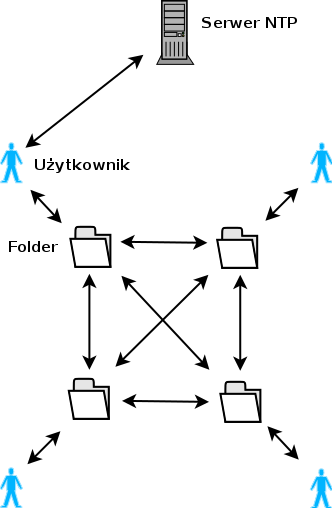
\includegraphics[width=200pt]{figures/model.png}
  \end{center}
  \caption{Model systemu \emph{TeamSync}.}
\end{figure}

Komunikacja i wymiana danych pomiędzy użytkownikami zachodzi tylko i wyłącznie poprzez aplikację BitTorrent Sync. Wymiana danych odbywa się automatycznie w momencie umieszczenia przez użytkownika nowych plików we wskazanym wcześniej folderze, lub w chwili modyfikacji już istniejących danych wewnątrz niego. Na poziomie transportu danych, jest on realizowany za pomocą protokołu BitTorrent.

Głównym obiektem, wewnątrz którego dane są obustronnie synchronizowane, jest folder --- w dalszej części pracy zastępowany również słowem ,,katalog'' o tożsamym znaczeniu. Po synchronizacji folderów każdy z węzłów posiada pełną kopię uwspólnianych danych wewnątrz swojego lokalnego folderu. Użytkownicy łączą wzajemnie swoje katalogi poprzez podanie ciągu 32 znaków (jest to tzw. \emph{secret}), za pomocą którego narzędzie BitTorrent Sync na jednym węźle jest w stanie odszukać u innego użytkownika zdalny folder, który oznaczony jest tym samym \emph{secretem}. 

System BitTorrent Sync gwarantuje natychmiastowe rozpoczęcie synchronizacji wszystkich danych wewnątrz folderu pomiędzy grupą połączonych ze sobą użytkowników. Wymiana danych pomiędzy dwoma węzłami odbywa się bezpośrednio --- bez serwera --- i nie jest możliwa, jeśli nie mają one możliwości nawiązania połączenia. Dodatkową konsekwencją takiej sytuacji jest fakt, że aby rozpropagowanie modyfikacji danych w sieci mogło mieć miejsce, przynajmniej dwaj użytkownicy muszą być do niej podłączeni.

Katalog synchronizowany przez użytkowników jest folderem zawierającym dowolną ilość danych, ograniczoną wyłącznie przez ilość dostępnej pamięci w systemie operacyjnym użytkownika. Pliki i katalogi wewnątrz współdzielonego folderu mogą być dowolnego typu, a dowolność ich nazw ogranicza jedynie system operacyjny.

\section*{Spójność wymienianych danych}

Użytkownicy synchronizujący ze sobą dane wewnątrz folderów --- ze względu na częstą zmianę dostępności każdego z węzłów --- narażeni są na wiele sytuacji grożących brakiem spójności wymienianych danych. Każdy z użytkowników posiada swoją lokalną, pełną kopię uwspólnionych plików. Podczas modyfikacji jednego z nich, zmiany rozsyłane są do pozostałych \emph{obecnych w danym momencie w sieci} węzłów --- w przypadku nieobecności dowolnego z użytkowników, zmiana zostanie odłożona w czasie do momentu, w którym będzie on dostępny w sieci. Wówczas --- o ile dowolny z węzłów posiadający dane po zmianie również jest obecny w sieci --- zmiany zostają natychmiast rozpropagowane.

Dodatkowo im więcej węzłów posiadających zmodyfikowane dane jest w sieci, tym szybciej dane będą się synchronizować. Dzieje się tak dlatego, że do transportu użyto protokołu \emph{BitTorrent}, za pomocą którego pobierane są drobne fragmenty danych od wszystkich dostępnych węzłów je posiadających, a dopiero po pobraniu fragmentów następuje łączenie ich w całość. Pozwala to na znacznie szybszą i bezpieczniejszą wymianę danych pomiędzy użytkownikami wewnątrz systemu \emph{BitTorrent Sync}, ponieważ fragmenty danych pobierane są od pozostałych węzłów równolegle.

Jednak pomimo cennych korzyści, podstawową trudnością jest zachowanie spójności w rozproszonym systemie. \emph{BitTorrent Sync} gwarantuje, że po uspójnieniu danych przez wszystkich użytkowników w systemie --- niezależnie od wcześniejszych różnic w przechowywanych lokalnie danych --- wszyscy użytkownicy ostatecznie będą posiadali \emph{jednakową} kopię danych. Ich lokalne zmiany, które nie zostały rozpropagowane w sieci zostaną dodane do katalogu \texttt{.sync} wewnątrz synchronizowanego katalogu, aby nie utracili oni swoich wersji zmodyfikowanych danych. Zawartość katalogu \texttt{.sync} nie jest przesyłana w sieci --- każdy węzeł ma inną jego zawartość.

\section*{Komunikacja między użytkownikami}

Podstawowymi obiektami, za pomocą których użytkownicy mogą się porozumiewać, są komentarze. Komentarz można umieścić w systemie \emph{TeamSync} za pomocą interfejsu graficznego, który dodaje go w odpowiedni sposób do systemu plików synchronizowanego folderu i rozsyła do pozostałych węzłów w sieci. Komentarz może zostać umieszczony w systemie przez dowolnego użytkownika, natomiast fizycznie w systemie przechowywany jest jako plik (na jeden komentarz w systemie przypada jeden plik) zawierający w sobie takie informacje jak:

\begin{itemize}[noitemsep]
 \item treść wypowiedzi,
 \item data i czas zamieszczenia,
 \item identyfikator autora,
 \item listę osób, które odczytały komentarz,
 \item historię zmian (poprzednia treść oraz data i czas zmiany).
\end{itemize}

Komentarze --- w dalszej części pracy nazywane również ,,wypowiedziami'', lub ,,postami'' --- zgrupowane są w większe struktury nazwane wątkami. Jeden wątek --- w dalszej części pracy nazywany też ,,dyskusją'' --- może zawierać w sobie nieograniczoną ilość wypowiedzi i może zostać oznaczony w systemie jako dyskusja na temat konkretnego (wybranego przez autora wątku) pliku znajdującego się w folderze.

W systemie wątek reprezentowany jest przez specjalnie oznaczony (za pomocą jego nazwy) katalog, wewnątrz którego znajdują się pliki z komentarzami. Dodatkowo, wewnątrz folderu przechowującego wątek, pomiędzy plikami z komentarzami znajduje się plik zawierający podstawowe informacje o wątku, między innymi:

\begin{itemize}[noitemsep]
 \item tytuł dyskusji,
 \item identyfikator autora,
 \item data i czas rozpoczęcia watku,
 \item plik, którego wątek dotyczy.
\end{itemize}

\begin{figure}[htb]
  \vspace{5pt}
  \begin{center}
    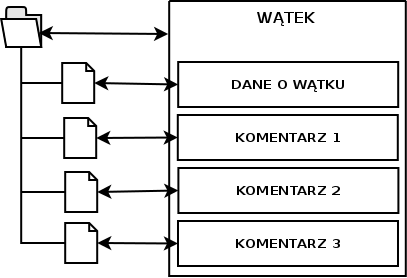
\includegraphics[width=240pt]{figures/folder-thread.png}
  \end{center}
  \caption{Odwzorowanie fizycznego składowania plików z komentarzami w wątku na logiczną ich reprezentację w systemie.}
\end{figure}

Na powyższym rysunku zaprezentowano, w jaki sposób fizycznie przechowywane są komentarze i w jaki sposób logicznie udostępniane są użytkownikom w systemie. Na jego podstawie można opisać kolejne założenie systemu, stanowiące o tym, że nie ma możliwości, aby w systemie komentarze istniały bez wątku --- przynależność wypowiedzi do dyskusji jest obligatoryjna.

Użytkownik może mieć wiele (maksymalnie $10$) folderów współdzielonych, każdy z innymi węzłami. Z tego powodu w modelu uwzględniono tzw. ,,tożsamości''. Tożsamość to nazwa użytkownika wpisywana przez niego podczas dołączania do folderu, która jest wyświetlana innym użytkownikom. Jedna tożsamość obowiązuje w jednym folderze i nie ma ograniczeń dotyczących powtarzalności --- użytkownik może w każdym uwspólnianym folderze mieć identyczną wyświetlaną nazwę.

Model systemu zakłada, że pliki raz zamieszczone w folderze nie będą zmieniać swojej lokalizacji wewnątrz niego. Założenie to może nie być przestrzegane tylko w przypadku, gdy żaden z wątków nie dotyczy przenoszonego pliku. W przeciwnym wypadku --- jeśli plik zmieni lokalizację (nawet pozostając nadal w uwspólnionym folderze) albo nazwę --- dyskusja dotycząca pliku nie zostanie wyświetlona. Powyższe założenie nie wnosi negatywnego działania w odniesieniu do synchronizowanych danych --- dotyczy wyłącznie funkcjonalności komentowania.

Wszystkie dane służące do obsługi systemu \emph{TeamSync} --- komentarze, pliki z danymi wątku, pliki przechowujące informacje o użytkownikach, pliki konfiguracyjne --- zapisywane są w formie słownika według formatu \texttt{JSON}. Każdy ze słowników zawiera klucze (ciągi znaków określające daną właściwość) oraz ich wartości.
\chapter{Ogólna koncepcja i architektura}

Aplikacja \emph{TeamSync} zrealizowana w ramach niniejszej pracy ma strukturę dwuwarstwową. Strony serwera oraz klienta, na wzór serwisów internetowych, są od siebie odizolowane, a komunikacja między nimi zachodzi z wykorzystaniem protokołu \texttt{HTTP} \cite{http} \cite{httparticle}. BitTorrent Sync jest narzędziem współpracującym z aplikacją, które jest odpowiedzialne za wymianę danych (synchronizację). Komunikacja z tym narzędziem jest możliwa dzięki odpowiednio skonfigurowanemu API, które zostało udostępnione przez twórców całego systemu.

Działanie aplikacji \emph{TeamSync} polega na uruchomieniu w tle systemu synchronizującego dane i udostępnienie użytkownikowi wygodnego interfejsu do umieszczania i odczytywania komentarzy, co odbywa się poprzez odpowiednią manipulację plikami wewnątrz synchronizowanych folderów. Jedyną drogą wymiany danych jest wspomniany system BitTorrent Sync.

\begin{figure}[htb]
  \vspace{5pt}
  \begin{center}
    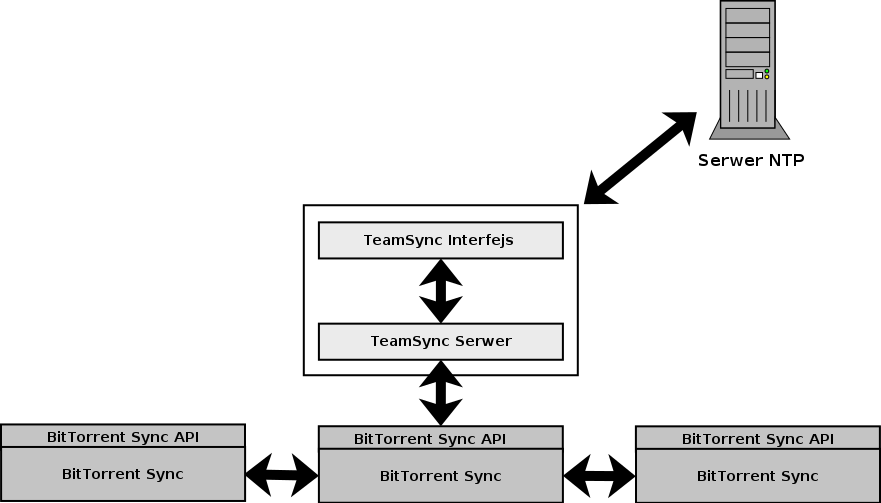
\includegraphics[width=380pt]{figures/architecture3.png}
  \end{center}
  \caption{Uproszczona architektura systemu \emph{TeamSync}.}
  \label{architecturepic}
\end{figure}

Poniżej zostaną omówione w oddzielnych podrozdziałach poszczególne moduły architektury systemu: BitTorrent Sync, system \emph{TeamSync} wraz z komunikacją pomiędzy jego częścią serwerową a kliencką oraz serwer NTP.

\section{BitTorrent Sync}

W poniższej sekcji opisanych zostanie kilka aspektów zarówno systemu BitTorrent Sync, jak i zaimplementowanemu przez jego twórców API, dzięki któremu możliwe jest wykonywanie większości funcji tego systemu z poziomu kodu. Rozdział rozpocznie sekcja \emph{secret} opisująca łańcuch znaków wymieniany między użytkownikami, po której zostanie przedstawiony bardziej szczegółowy opis protokołu komunikacji z systemem BitTorrent Sync.

\subsection{Secret}

\label{secret}

W aplikacji BitTorrent Sync \emph{secret} jest ciągiem $32$ znaków, służącym do identyfikacji synchronizowanych folderów. Dodając katalog do tego systemu, użytkownik może posłużyć się istniejącym już \emph{secretem}, jeśli otrzymał go od użytkownika, który wcześniej zainicjował folder. Może też sam go zainicjować, generując \emph{secret} tworząc losowy ciąg znaków odpowiadający wyrażeniu regularnemu \texttt{[A-Z0-9]\{32\}}, co odpowiada trzydziestu dwóm losowym znakom wybranym ze zbioru cyfr od $0$ do $9$ oraz liter alfabetu od \texttt{A} do \texttt{Z}.

Duża ilość znaków ($32$ znaki) oraz duży ich zbiór ($24$ litery $+$ $10$ cyfr daje łącznie moc zbioru znaków równą $34$) powodują, że istnieje znikoma szansa na powtórzenie się dwóch łańcuchów znakowych.

Podczas generowania wartości \emph{secret}, tworzone są dwa łańcuchy znaków o dwóch typach synchronizacji:

\begin{description}[noitemsep]
  \item[read\_write] --- użytkownicy, którzy otrzymają \emph{secret} pochodzący z tej wartości będą mogli zarówno odczytywać dane, jak i je modyfikować oraz dodawać swoje; modyfikacje danych --- w przeciwieństwie do trybu \texttt{read\_only} --- będą się propagować do pozostałych użytkowników,
  
  \item[read\_only] --- użytkownicy, którzy otrzymają ten \emph{secret}, będą mogli wyłącznie pobierać dane, nie mogąc ich modyfikować (niezależnie od modyfikacji, zmiany nie będą propagowane do innych użytkowników).
\end{description}

W zależności od tego, który z \emph{secretów} użytkownik otrzyma, tak system będzie uspójniał dane.

\subsection{Protokół BitTorrent Sync API}

\label{btsyncapiproto}

Twórcy systemu BitTorrent Sync umożliwili korzystanie z dodatkowej funkcjonalności aplikacji nie tylko użytkownikom, ale również programistom chcącym testować lub udoskonalać narzędzia związane z wymianą plików. Sterowanie systemem z poziomu kodu jest możliwe dzięki zaimplementowanemu przez twórców aplikacji API, które umożliwia komunikację pomiędzy narzędziem a stworzoną przez programistę aplikacją.

API narzędzia odbiera żądania --- z odpowiednio dobranymi parametrami --- nasłuchując na porcie wskazanym przez użytkownika w pliku konfiguracyjnym (dokładny opis pliku konfiguracyjnego znajduje się w podrozdziale \ref{configbtsync}). Pełen adres, na który programista musi skierować żądanie HTTP ma postać wzorca:
\begin{verbatim}
                          http://<adres>:<port>/api
\end{verbatim}

W przypadku aplikacji \emph{TeamSync} zaimplementowanej w ramach niniejszej pracy magisterskiej, ze względu na lokalizację systemu BitTorrent Sync (lokalna maszyna) użyty adres to \texttt{localhost} oraz port \texttt{8787} (zmieniony z domyślnego \texttt{8888} ze względu na jego dużą popularność w aplikacjach). Pełen adres, na który są wysyłane żądania pomiędzy aplikacją \emph{TeamSync}, a API systemu BitTorrent Sync to:
\begin{verbatim}
                          http://localhost:8787/api
\end{verbatim}

\subsubsection*{Komunikaty BitTorrent Sync API}

Żądania wysyłane z systemu \emph{TeamSync} do API zawierają w nagłówku parametr uwierzytelniający \emph{Basic HTTP Authentication} \cite{basicauth}. Dane dostępu zawierają wartości \texttt{login} oraz \texttt{password}, które --- aby zostały poprawnie odebrane --- muszą odpowiadać danym umieszczonym wewnątrz pliku konfiguracyjnego systemu BitTorrent Sync. Uruchamiając po raz pierwszy aplikację \emph{TeamSync} dane uwierzytelniające są tworzone wraz z plikami konfiguracyjnymi i ustawione domyślnie na \texttt{team} oraz \texttt{sync} odpowiednio dla wartości \texttt{login} oraz \texttt{password}.

Zapytania przyjmowane przez BitTorrent Sync API zawierają dodatkowo tzw. ,,metodę'' wraz z jej argumentami. Metoda oznacza funkcję, która zostanie wykonana na podanych argumentach np. pobieranie listy folderów wprowadzonych do systemu i współdzielonych z innymi użytkownikami, pobieranie listy użytkowników, z którymi użytkownik synchronizuje dany folder, zwrócenie ustawień konkretnego folderu lub ich zmiana i wiele innych. W aplikacji \emph{TeamSync} użyto niewielkiej ilości możliwych metod ze względu na ich dużą liczebność i użyteczność odbiegającą od głównego celu projektu.

Użyte metody wraz z typem przyjmowanych argumentów zostaną opisane w oddzielnych sekcjach. Wszystkie zwroty użyte w poniższych podrozdziałach dotyczące aplikacji takie jak: ,,aplikacja'', ,,system'', ,,narzędzie'', będą dotyczyły systemu BitTorrent Sync. Sposób działania narzędzia zaimplementowanego w ramach niniejszej pracy nie będzie omawiany podczas opisu poniższych metod.

Przykłady dotyczące sposobu wysyłania zapytań przez aplikację \emph{TeamSync} są napisane według wzoru podyktowanego przez wymagania funkcji pakietu \texttt{requests} języka \emph{Python}, które zostały użyte do wysyłania żądań do BitTorrent Sync API.

\begin{minipage}{\linewidth}
\vspace{15pt}
\begin{verbatim}
            requests.get('http://adres:port/api',
                         auth=('login', 'password'),
                         params={
                             'method': 'nazwa_metody',
                             'arg1': 'wartość_argumentu',
                             [ . . . ]
                         }
            )
\end{verbatim}
\vspace{15pt}
\end{minipage}

Pierwszy argument wewnątrz zapytania reprezentuje adres wraz z numerem portu, na który zostanie wysłane żądanie. Dane uwierzytelniające przesyłane są wewnątrz parametru \texttt{auth}, natomiast nazwa metody oraz pozostałe argumenty przesyłane są wewnątrz parametru \texttt{params}, który ma strukturę słownika z nazwą oraz wartością poszczególnych argumentów.

\subsubsection*{\emph{get\_secrets}}

\label{getsecrets}

Metoda \emph{get\_secrets} nie wymaga żadnych dodatkowych argumentów i służy do generowania przez aplikację ciągów znakowych identyfikujących synchronizowany folder.  Zapytanie wysyłane do BitTorrent Sync API w celu ich uzyskania:

\begin{minipage}{\linewidth}
\vspace{15pt}
\begin{verbatim}
               requests.get('http://localhost:8787/api',
                            auth=('team', 'sync'),
                            params={
                                'method': 'get_secrets',
                            }
               )
\end{verbatim}
\vspace{15pt}
\end{minipage}

Odpowiedź aplikacji będąca słownikiem w formacie \texttt{JSON} \cite{jsonarticle} zawiera dwie wartości:

\begin{itemize}[noitemsep]
  \item \emph{read\_write} --- \emph{secret} służący do synchronizacji folderu w trybie zapisu/odczytu,
  \item \emph{read\_only} --- \emph{secret}, za pomocą którego użytkownik może udostępnić swoje dane, nie pozwalając na modyfikację lub dodawanie danych innym użytkownikom.
\end{itemize}

\subsubsection*{\emph{add\_folder}}

Metoda dodająca wskazany w argumencie folder do systemu. Po otrzymaniu żądania zawierającego tę metodę, do wybranego katalogu --- który w momencie wykonywania metody musi być pusty (wymaganie systemu BitTorrent Sync) --- aplikacja dodaje ukryty folder \texttt{.sync} (dokładny opis zawartości katalogu \texttt{.sync} znajduje się w podrozdziale \ref{directorystructure}) i od tego momentu katalog wskazany w żądaniu będzie włączony do synchronizacji.

Oprócz metody komunikat zawiera dodatkowe parametry:

\begin{itemize}[noitemsep]
  \item \emph{dir} --- pełna ścieżka do folderu,
  \item \emph{secret} --- losowy ciąg znaków będący tzw. ,,secretem'', za pomocą którego możliwa jest synchronizacja katalogów między użytkownikami. Jeśli parametr ten pozostanie pusty, system otrzyma informację, że folder jest nowy i nie jest jeszcze synchronizowany przez żadnego z użytkowników. Aplikacja wygeneruje secret i od tego momentu użytkownik może przekazywać go innym węzłom, aby współdzielić wskazany katalog.
\end{itemize}

Zakładając, że synchronizowany ma zostać katalog o ścieżce \texttt{/home/user/testowy\_katalog}, zapytanie zostanie wysłane z serwera aplikacji \emph{TeamSync} w następujący sposób:

\begin{minipage}{\linewidth}
\vspace{15pt}
\begin{verbatim}
     requests.get('http://localhost:8787/api',
                  auth=('team', 'sync'),
                  params={
                      'method': 'add_folder',
                      'dir': '/home/user/testowy_katalog',
                      'secret': 'A3LL43HJ257YCKMOLAD7QSEAS7U373BVO'
                  }
     )
\end{verbatim}
\vspace{15pt}
\end{minipage}

W przypadku otrzymania takiego komunikatu z pustym argumentem \texttt{secret}, aplikacja wygenerowałaby nowy secret i zwróciłaby go w odpowiedzi. W innym przypadku, w odpowiedzi przesyłany jest wyłącznie kod błędu wewnątrz zmiennej \texttt{error}. W przypadku otrzymanej wartości równej $0$ użytkownik jest informowany, że operacja dodawania nowego folderu przebiegła pomyślnie.

\subsubsection*{\emph{get\_folders}}

Za pomocą tej metody otrzymywana jest lista folderów, które zostały wprowadzone do systemu. Podobnie jak przy metodzie \emph{get\_secrets} żadne dodatkowe argumenty nie są wymagane.

\begin{minipage}{\linewidth}
\vspace{15pt}
\begin{verbatim}
               requests.get('http://localhost:8787/api',
                            auth=('team', 'sync'),
                            params={
                                'method': 'get_folders',
                            }
               )
\end{verbatim}
\vspace{15pt}
\end{minipage}

W odpowiedzi na zapytanie \emph{get\_folders} BitTorrent Sync API zwraca listę, wewnątrz której znajdują się informacje o wszystkich synchronizowanych w systemie folderach w formacie \texttt{JSON}. Wśród kluczy słowników są:

\begin{itemize}[noitemsep]
  \item \emph{error} --- w przypadku niepowodzenia przesyłana jest tylko ta wartość ustawiona na $1$; w przypadku powodzenia wartość $0$,
  
  \item \emph{dir} --- bezwzględna ścieżka folderu w systemie plików lokalnego użytkownika,
  
  \item \emph{files} --- liczba plików, które znajdują się wewnątrz folderu,
  
  \item \emph{size} --- łączny rozmiar plików wewnątrz folderu w bajtach,
  
  \item \emph{secret} --- łańcuch znaków służący do identyfikacji współdzielonych folderów między zdalnymi użytkownikami (więcej w sekcji \ref{secret}),
  
  \item \emph{type} --- rodzaj synchronizacji; możliwe dwie wartości:
  \begin{itemize}[noitemsep]
    \item \emph{read\_write} --- użytkownicy mogą zarówno odczytywać, jak i modyfikować pliki,
    
    \item \emph{read\_only} --- tylko właściciel może modyfikować, pozostali użytkownicy wyłącznie odczytywać,
  \end{itemize}
  
  \item \emph{down\_speed} --- chwilowa prędkość pobierania; jeśli wszystkie dane w folderze są zsynchronizowane, wartość $0$,
  
  \item \emph{up\_speed} --- chwilowa prędkość wysyłania; jeśli wszystkie dane w folderze są zsynchronizowane, wartość $0$,
  
  \item \emph{id} --- unikalny identyfikator folderu, który może różnić się pomiędzy użytkownikami.
\end{itemize}

Przykładowa odpowiedź BitTorrent Sync API na powyższe żądanie może wyglądać następująco:

\begin{minipage}{\linewidth}
\vspace{15pt}
\begin{verbatim}
         [
             {
                 "error": 0, 
                 "dir": "/home/user/testowy katalog", 
                 "files": 9, 
                 "size": 3079, 
                 "secret": "A3LL43HJ257YCKMOLAD7QSEAS7U373BVO", 
                 "type": "read_write", 
                 "down_speed": 0, 
                 "up_speed": 0, 
                 "id": 902958156496830188
             }
         ]
\end{verbatim}
\vspace{15pt}
\end{minipage}

Otrzymanie takiej odpowiedzi wskazuje na fakt, iż jednym (i jedynym, ze względu na obecność tylko jednego obiektu typu \texttt{JSON} w liście katalogów) z synchronizowanych folderów w systemie jest folder o ścieżce \texttt{/home/user\-/testowy katalog}. Został on poprawnie odczytany przez system BitTorrent Sync (\texttt{'error': 0}) i zawiera dziewięć plików o łącznym rozmiarze $3079$ bajtów. Aby uwspólnić go z innymi użytkownikami w trybie umożliwiającym im zarówno odczyt, jak i modyfikację zawartości (tryb \texttt{read\_write}), należy przekazać \emph{secret} o wartości \texttt{A3LL43HJ\-257YCKMO\-LAD7QSEAS\-7U373BVO}.

Wartości \texttt{down\_speed} oraz \texttt{up\_speed} sugerują brak wymiany danych między użytkownikami w chwili wysyłania żądania \emph{get\_folders}. Wewnętrznym identyfikatorem folderu w systemie lokalnym użytkownika jest liczba \texttt{902958156496830188}.

\subsubsection*{remove\_folder}

Ostatnią z używanych przez system \emph{TeamSync} metod jest metoda \emph{remove\_folder}, która usuwa z systemu wskazany synchronizowany folder --- nie usuwa fizycznie katalogu z systemu plików, lecz blokuje jego dalszą synchronizację. Aby ponownie użyć tego samego katalogu, należy usunąć z niego wszystkie pliki (wymaganie aplikacji dotyczące pustego folderu). W parametrze żądania --- oprócz metody --- aplikacja potrzebuje wartość \emph{secret} folderu, który użytkownik zamierza usunąć.

\begin{minipage}{\linewidth}
\vspace{15pt}
\begin{verbatim}
       requests.get('http://localhost:8787/api',
                    auth=('team', 'sync'),
                    params={
                        'method': 'remove_folder',
                        'secret': 'A3LL43HJ257YCKMOLAD7QSEAS7U373BVO'
                    }
       )
\end{verbatim}
\vspace{15pt}
\end{minipage}

W przeciwieństwie do metody \emph{add\_folder}, w której parametr \emph{secret} był opcjonalny, tutaj konieczne jest przesłanie tego parametru. Jeśli nie zostanie on przesłany lub okaże się niepoprawny, aplikacja zwróci kod błędu w zmiennej \texttt{error}. W przypadku poprawnego przebiegu operacji \emph{remove\_folder}, kod błędu będzie równy $0$.

\section{\emph{TeamSync}}

\label{teamsyncarch}

Po opisaniu modułu BitTorrent Sync API z Rys. \ref{architecturepic} umieszczonego no początku rozdziału, przedstawiony zostanie dokładniej sposób działania systemu \emph{TeamSync} --- jak zapisywane są komentarze oraz wątki, jak są przekazywane w sieci oraz w jaki sposób system unika konfliktów.

\subsection{Komentarze}

\label{archcomments}

Rozproszona architektura nie daje pewności, że modyfikacja pliku odbędzie się bezkonfliktowo, ponieważ zawsze może wystąpić sytuacja, w której inny węzeł ,,równocześnie'' (pod względem zegara logicznego, nie czasu rzeczywistego) nie dokona edycji danych. Podczas testów aplikacji BitTorrent Sync, która jest odpowiedzialna za wymianę danych --- a więc również za rozwiązywanie konfliktów --- nie wyizolowano priorytetów określających, którą wersję i z którego węzła należy usunąć, a z którego rozpropagować.
 
Z powyżej opisanych powodów umieszczanie komentarzy w aplikacji \emph{TeamSync} polega na \emph{dodawaniu} nowych plików przez użytkowników. Algorytm dodawania nowego komentarza z lokalnej perspektywy wygląda następująco:

\begin{enumerate}[noitemsep]
 \item Pobierz znacznik czasowy z serwera NTP.
 
 \item Umieść pobrane od użytkownika dane (treść komentarza, identyfikator) oraz pobrany wcześniej znacznik czasowy do zmiennej o strukturze słownika (JSON).
 
 \item Zapisz słownik do pliku o nazwie złożonej ze znacznika czasowego oraz identyfikatora użytkownika wewnątrz katalogu z wątkiem.
\end{enumerate}

Umieszczenie komentarza w systemie i rozpropagowanie go pomiędzy wszystkich aktywnych użytkowników zaprezentowane jest na rysunku \ref{rys:writecomment}.

\begin{figure}[t]
  \vspace{5pt}
  \begin{center}
    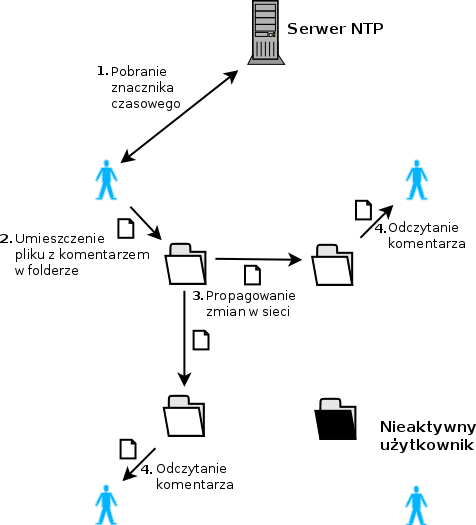
\includegraphics[width=220pt]{figures/writecomment.png}
  \end{center}
  \caption{Uproszczony schemat dodawania nowego komentarza do systemu i odczytanie go przez aktywnych użytkowników.}
  \label{rys:writecomment}
\end{figure}

\subsubsection*{Struktura komentarzy}

Wszystkie zapisywane komentarze mają swoją strukturę, która --- podobnie jak w przypadku wszystkich danych przesyłanych i zapisywanych do plików w aplikacji \emph{TeamSync} --- jest strukturą słownikową zapisaną w formacie JSON. Każdy plik komentarza zawiera pięć kluczy wraz z wartościami:

\begin{itemize}[noitemsep]
 \item \emph{comment} --- treść komentarza,
 
 \item \emph{timestamp} --- znacznik czasowy pobierany podczas powstawania komentarza,
 
 \item \emph{history} --- lista zawierająca obiekty o strukturze słownikowej, które przechowują wszelkie zmiany treści komentarza w wartościach kluczy \texttt{comment} oraz \texttt{timestamp}. W momencie zmiany treści przez autora wypowiedzi, dodawany jest nowy element w liście \texttt{history} z obiektem o tych kluczach z wartościami wypełnionymi nową treścią (\texttt{comment}) oraz nowym znacznikiem czasowym (\texttt{timestamp}),
 
 \item \emph{uid} --- autor komentarza,
 
 \item \emph{readby} --- zmienna o strukturze słownika przechowująca informację o użytkownikach, którzy odczytali komentarz i o czasie, w którym to zrobili. W kluczu znajduje się identyfikator autora, natomiast jako wartość wpisywany jest znacznik czasowy odczytania posta.
\end{itemize}

Po zatwierdzeniu zmiany wyświetlana jest najnowsza treść komentarza, natomiast znacznik czasowy pozostaje bez zmian. Taka implementacja jest wymuszona przez konieczność zachowania ciągłości logicznej konwersacji --- edytowany post nie może przemieszczać się w chronologicznym porządku wymiany opinii, ponieważ część wypowiedzi może zostać źle odczytana w przypadku modyfikacji komentarzy przed nią. Intencje edycji zazwyczaj polegają na korygowaniu napisanych wcześniej zdań (interpunkcja, ,,literówki'', ortografia) lub dodawaniu mniej znaczących faktów --- rzadko zdarza się całkowita modyfikacja treści, a w przypadku gdy jednak wystąpi, użytkownicy mogą przejrzeć historię komentarzy, gdy dostrzegą logiczne niezgodności w przepływie opinii.

\subsubsection*{Konflikty}

Struktura pliku z komentarzem może być bardzo dynamiczna i często zmieniana, ponieważ istnieje lista (\texttt{history}), w której dodawane sa elementy, oraz słownik (\texttt{readby}) uzupełniany o kolejne pary klucz-wartość. Czy wobec tego nie generuje to konfliktów, które mogłyby naruszyć spójność danych? Czy użytkownik \texttt{A} może znaleźć się w sytuacji, że ,,ominie'' go część informacji, gdy użytkownik \texttt{B} nadpisze swoją część zamiast części użytkownika \texttt{C}? Lub czy jest możliwość, że modyfikacja użytkownika \texttt{A} zostanie pominięta, ponieważ w tym samym czasie użytkownik \texttt{B} dokonał zmian w tym samym komentarzu i ,,wygrał'' synchronizację?

Odpowiedź brzmi: TAK, jest taka możliwość.

Modyfikacja komentarzy zachodzi w dwóch przypadkach: edycji treści oraz odczytaniu go przez użytkownika. Poniżej zostaną rozważone obydwa przypadki i w każdym z nich opisane zostaną możliwości konfliktów oraz ich skutki.

\begin{description}[noitemsep]
  \item[Modyfikacja treści] --- wystąpienie konfliktu w przypadku edytowania treści jest niemożliwe, ponieważ interfejs użytkownika pozwala na poprawienie treści tylko w przypadku, gdy jesteś autorem komentarza. Jeden użytkownik nie jest w stanie dokonać edycji dwóch postów jednocześnie.
  
  \item[Odznaczenie jako przeczytane] --- w tym przypadku konflikt może wystąpić, lecz nie będzie miał żadnych poważnych konsekwencji. Żeby to wyjaśnić, załóżmy, że użytkownicy \texttt{A} oraz \texttt{B} nie przeczytali jeszcze pewnego komentarza \texttt{x} i zrobią to w tym samym momencie (albo każdy z nich zrobi to na swojej lokalnej wersji, gdy żaden z pozostałych użytkowników należących do folderu nie będzie dostępny). W obecnej chwili (przed wzajemną synchronizacją) obydwaj użytkownicy mają oznaczony post \texttt{x} jako przeczytany. W momencie synchronizacji ,,wygra'' wersja pliku któregoś z użytkowników. Załóżmy, że wygra użytkownik \texttt{A}: wówczas użytkownik \texttt{B} zobaczy w swojej aplikacji \emph{TeamSync}, że ponownie ma nieprzeczytany komentarz, ale wówczas znowu aplikacja ,,przeczyta'' komentarz ponownie odpowiednio go modyfikując (wstawiając nową parę klucz-wartość do słownika \texttt{readby}).
  
  Nawet w przypadku częstych konfliktów, wpływa to nieznacznie tylko i wyłącznie na wygodę użytkownika (ponowne ,,kliknięcie'' na nieprzeczytany wątek).
\end{description}

\subsubsection*{Przykładowy komentarz}

Na rysunku \ref{rys:comment} przedstawiona została struktura komentarza, który dla lepszego zobrazowania własnej struktury został odczytany przez trzech użytkowników i był modyfikowany dwukrotnie.

\begin{figure}[t]
  \label{rys:comment}
  \begin{verbatim}
            {
                "comment": "Ostateczna treść komentarza", 
                "timestamp": "1439395604000", 
                "history": [
                    {
                        "comment": "Pierwsza treść", 
                        "timestamp": "1439395604000"
                    },
                    {
                        "comment": "Pierwsza treść zmodyfikowana", 
                        "timestamp": "1439395945000"
                    },
                    {
                        "comment": "Ostateczna treść komentarza", 
                        "timestamp": "1439396291000"
                    }
                ], 
                "uid": "2HI7KRUNSSONIUJKMRWXGOTIZSHBGFIH", 
                "readby": {
                    "2HI7KRUNSSONIUJKMRWXGOTIZSHBGFIH": "1439395604000",
                    "2SAFDSBCXGFD765GDFS4GFDS35FDSBVB": "1439395888000",
                    "3REW54GFDS6578FDSGDF5BSH652F2B34": "1439396782000"
                }
            }
  \end{verbatim}
  \caption{Struktura przykładowego komentarza.}
\end{figure}

W poniższym przykładzie dobrze widać zmianę treści komentarza poprzez pobranie jej z najświeższej modyfikacji oraz niezmienność znacznika czasowego (\texttt{timestamp}) niezależnie od tego, czy komentarz był modyfikowany. Zauważalna jest też łatwość, z jaką można odtworzyć całą historię zmian wypowiedzi. Oglądanie zmian wszystkich komentarzy jest dostępne dla każdego z użytkowników niezależnie od przynależności, o ile taka historia dla konkretnego przypadku istnieje.

Dzięki słownikowi \texttt{readby} można odczytać, który z użytkowników i w jakim czasie odczytał ten komentarz: na przykład użytkownik o identyfikatorze \texttt{2HI7KRUN\-SSONIUJ\-KMRWXGOTI\-ZSHBGFIH} podczas odczytywania wypowiedzi umieścił swój wpis, pobierając znacznik czasowy \texttt{1439395604000}, co odpowiada dacie \texttt{12.08.2015r.} i godzinie \texttt{18:06} czasu polskiego.

\subsection{Wątki}

Wewnątrz każdego folderu z wątkiem oprócz plików z komentarzami znajduje się plik o nazwie \texttt{meta}, który zawiera dane związane z wątkiem prezentowane w interfejsie użytkownika. Podobnie jak w przypadku komentarzy, są one ustrukturyzowane jako para klucz/wartość w formacie JSON. Klucze znajdujące się w pliku \texttt{meta} obejmują następujące informacje:

\begin{itemize}[noitemsep]
  \item \emph{uid} --- autor wątku,
  \item \emph{timestamp} --- znacznik czasowy pobrany podczas tworzenia wątku (identyczny ze znacznikiem czasowym pierwszego komentarza),
  \item \emph{fileabout} --- ścieżka wewnątrz folderu wskazująca na plik, którego dotyczy watek,
  \item \emph{topic} --- tytuł watku.
\end{itemize}

Plik \texttt{meta} został wprowadzony w celu szybszego odczytywania listy wątków --- podczas przygotowywania listy, odczytywanie przez aplikację komentarzy jest niepotrzebne, dzięki czemu aplikacja działa szybciej. Pobieranie komentarzy z folderu zawierającego wątek (treści, znaczników czasowych itd.) następuje \emph{po} wybraniu konkretnej dyskusji.

Informacje dodatkowe wątku (np. ilość napisanych komentarzy, znacznik czasowy najświeższego komentarza) są na bieżąco obliczane przez aplikację podczas pobierania listy wątków. Znaczniej łatwiej (oraz szybciej) byłoby zapisać te dane w pliku \texttt{meta} i odczytywać je z otwartego już pliku. Natomiast wówczas pojawiłaby się możliwość wystąpienia konfliktów podczas jego edycji. Węzeł, który dodawałby nowy komentarz, musiałby edytować plik \texttt{meta} i inkrementować licznik komentarzy oraz zmodyfikować czas najświeższego komentarza. W przypadku dwóch użytkowników dodających komentarz w tym samym czasie dochodziłoby do konfliktów i umieszczania fałszywych danych wewnątrz pliku.

Dwie z informacji o wątku --- autor oraz znacznik czasowy --- są powielone z pierwszego komentarza w dyskusji (ponieważ podczas zakładania wątku umieszczany jest również inicjujący go komentarz). Zaimplementowano to w taki sposób, aby mieć dostęp do danych o wątku bez konieczności odczytywania któregokolwiek z komentarzy (np. odczytanie pierwszego komentarza wymaga sortowania, ponieważ funkcja modułu \texttt{os} języka \emph{Python} o nazwie \texttt{listdir} listuje nieuporządkowaną zawartość katalogu przyjmowanego w argumencie.

\subsubsection*{Przykładowy plik \texttt{meta}}

Poniżej przedstawiony został przykładowy plik z metadanymi wątku o nazwie ,,Przykładowy wątek''.

\begin{figure}[htb]
  \label{thread}
  \begin{verbatim}
                  {
                      "topic": "Przykładowy wątek", 
                      "timestamp": "1439395604000", 
                      "fileabout": "/katalog1/test.txt",
                      "uid": "2HI7KRUNSSONIUJKMRWXGOTIZSHBGFIH", 
                  }
  \end{verbatim}
  \caption{Struktura przykładowego pliku z metadanymi wątku.}
\end{figure}

Według tego przykładowego pliku wątek został utworzony --- zgodnie ze znacznikiem czasowym --- 30. sierpnia 2015 r. o godzinie \texttt{9:23}. Autorem jest użytkownik o identyfikatorze \texttt{2HI7KRU\-NSSONIUJ\-KMRWXGOTI\-ZSHBGFIH}. Dyskusja o tytule ,,Przykładowy wątek'' rozpoczęta przez tego użytkownika dotyczy pliku \texttt{test.txt}, który znajduje się wewnątrz folderu \texttt{katalog1} wewnątrz folderu synchronizowanego.

Strukturę przykładowego synchronizowanego folderu --- zawierający zarówno wątek z powyższego przykładu jak i plik opisywany w dyskusji --- przedstawiono poniżej:

\begin{minipage}{\linewidth}
\vspace{1em}
\begin{verbatim}
    [root]/
        .sync/
            [ pliki aplikacji BitTorrent Sync ]
        .Users/
            [ pliki z danymi o użytkownikach ]
        .Comments/
            katalog1/
                1439395604000@#&$Przykładowy wątek/
                    meta
                    1439395604000@#&$2HI7KRUNSSONIUJKMRWXGOTIZSHBGFIH
            1439423576000@#&$Inny wątek/
                meta
                1439423576000@#&$2SAFDSBCXGFD765GDFS4GFDS35FDSBVB
                1439476598000@#&$2HI7KRUNSSONIUJKMRWXGOTIZSHBGFIH
        katalog1/
            test.txt
            ccc.txt
        aaa.txt
        bbb.txt
\end{verbatim}
\vspace{1em}
\end{minipage}

Widać wewnątrz poniższej struktury, że ,,Przykładowy wątek'' został umieszczony w folderze \texttt{.Comments} w lokalizacji takiej samej, jak oryginalny plik, o którym powstała dyskusja (\texttt{katalog1}). Wewnątrz niego znajduje się plik z metadanymi o wcześniej przedstawionej strukturze oraz jeden komentarz. Warto zauważyć, że w nazwie komentarza jest ten sam znacznik czasowy, który jest zapisany w pliku \texttt{meta} --- według zasad opisanych wcześniej.

W przykładzie umieszczono również drugi wątek, zlokalizowany najpłycej w katalogu \texttt{.Comments}. Oznacza to, że w interfejsie graficznym będzie on wylistowany zawsze, gdy użytkownik nawigując po folderze, będzie przebywał na najwyższym jego poziomie --- ,,korzeniu''. ,,Inny wątek'' --- bo tak należy odczytać tytuł tej dyskusji, zawiera dwa komentarze --- jeden napisany przez użytkownika \texttt{2SAFDSB\-CXGFD765\-GDFS4GFDS\-35FDSBVB} w chwili pobrania znacznika czasowego \texttt{1439423\-576000} oraz przez użytkownika \texttt{2HI7KRU\-NSSONIUJ\-KMRWXGO\-TIZSHBGFIH} w chwili \texttt{1439476\-598000}.

\subsection{Nazwy folderów i plików}

\label{filenamesf}

Foldery zawierające wątki oraz pliki z komentarzami są tworzone przez dowolny węzeł w dowolnym czasie, co zwiększa niebezpieczeństwo wystąpienia konfliktów w nazwach tworzonych plików za każdym razem, gdy użytkownik wypowiada się w dyskusji lub rozpoczyna nową. Dodatkowo drzewiasta struktura katalogu \texttt{.Comments}, wewnątrz którego przechowywane są komentarze, powoduje, że ,,zwykłe'' foldery przechowywane są obok katalogów zawierających pliki komentarzy. Przeszukiwanie ich wszystkich przez serwer poprzez przeglądanie wszystkich lokalizacji jest wolniejsze i przy folderze mocno rozbudowanym systemem katalogów może odczuwalnie spowolnić aplikację.

Mając na uwadze powyższe problemy, projektując aplikację \emph{TeamSync} przyjęto następujące dwie zasady --- dotyczące nazw zarówno plików komentarzy, jak i folderów z wątkami --- jako konieczne do spełnienia. Konsekwencje nieprzestrzegania każdej z zasad będą wyjaśnione w dalszej części sekcji.

\begin{enumerate}[noitemsep]
  \item System powinien uniemożliwiać (zapewniać poziom prawdopodobieństwa \emph{w praktyce} uniemożliwiający) powtarzanie się \emph{nazwy} pliku komentarza lub folderu wątku.
  
  \item Nazwy powinny zawierać w sobie pewien element (ciąg znaków), dzięki któremu serwer odczyta informację, że wybrany folder lub plik to odpowiednio folder zawierający wątek oraz plik przechowujący wypowiedź. Informacja o wyjątkowości katalogu musi być zawarta w jego nazwie.
\end{enumerate}

Opisy sposobów realizacji obydwóch zasad zostały opisane w poniższych podrozdziałach.

\subsubsection*{Unikalność nazwy}

Jeśli w przypadku plików z komentarzami unikalność wprowadzanych nazw nie byłaby zachowana, efektem byłby konflikt skutkujący nadpisaniem pliku. Użytkownik \texttt{A} zatwierdzający treść odpowiedzi umieściłby swój plik, który chwilę później byłby nadpisany przez użytkownika \texttt{B}. Wersja użytkownika \texttt{A} zostałaby uznana jako nieaktualna i w konsekwencji przeniesiona do katalogu \texttt{Archive} w ukrytym folderze \texttt{.sync}, do którego użytkownicy nie mają dostępu z poziomu aplikacji \emph{TeamSync}.

Podobnie --- lecz z innymi konsekwencjami --- wygląda sytuacja w przypadku tworzenia nowego wątku. Gdyby ten sam użytkownik \texttt{A} tworzył nowy wątek w tym samym momencie, co użytkownik \texttt{B}, również wystąpiłby konflikt, lecz z odmiennymi skutkami. W kodzie serwera zastosowano instrukcję warunkową przed tworzeniem nowego folderu wątku sprawdzającą, czy taki folder już istnieje. Aplikacja tworzy nowy katalog, jeśli jeszcze nie istniał wcześniej w systemie plików --- w odwrotnym przypadku serwer kontynuuje działanie bez żadnych zmian. Efektem konfliktu byłoby nienadpisanie folderu z wątkiem, a nadpisanie pliku \texttt{meta} oraz (w zależności czy unikalność nazwy pliku z komentarzem została zachowana) możliwość nadpisania lub dodania nadmiarowego komentarza. W obecnym przypadku (użytkownicy \texttt{A} oraz \texttt{B} próbujący dodać nowy wątek w tym samym momencie) dodanie komentarza mogłoby skutkować następującą zawartością folderu z wątkiem:

\begin{itemize}[noitemsep]
  \item plik \texttt{meta} z treścią umieszczoną przez zwycięzcę konfliktu \texttt{A} vs. \texttt{B},
  
  \item komentarz użytkownika \texttt{A},
  
  \item komentarz użytkownika \texttt{B}.
\end{itemize}

Jak widać zapewnienie unikalności nazwy plików z komentarzami oraz folderów z wątkami w kontekście działania najważniejszej funkcjonalności jest niezbędne. Dlatego uzyskanie jednoznacznych nazw w przypadku plików z komentarzami odbywa się dzięki następującym składnikom:

\begin{itemize}[noitemsep]
  \item znacznik czasowy pobrany z serwera NTP podczas pisania nowego komentarza z dokładnością do jednej sekundy,
  
  \item identyfikator autora wypowiedzi (\emph{uid}).
\end{itemize}

Dzięki kombinacji tych dwóch składników nie ma możliwości uzyskać w systemie identycznej pary nazw pliku z komentarzem. Żeby złamać zasadę i uzyskać taką parę, ten sam użytkownik musiałby wysłać dwa komentarze w ciągu jednej sekundy, co --- ze względu na długość przetwarzania umieszczania odpowiedzi w systemie plików, oczekiwanie na odpowiedź ze znacznikiem czasowym z serwera NTP i otrzymania odpowiedzi przez klienta w przeglądarce --- jest bardzo mało prawdopodobne.

Nawet jeśliby tak się stało, druga wysłana przez użytkownika wypowiedź byłaby pusta, ponieważ nie miałby czasu na wypełnienie jej treścią --- interfejs graficzny automatycznie po zatwierdzeniu komentarza usuwa całą treść z pola tekstowego i jest gotowy do umieszczania następnej wypowiedzi. W momencie odnotowania przez serwer faktu, że komentarz ma pustą treść, przekaże błąd użytkownikowi za pomocą komunikatu: ,,\emph{Treść komentarza nie może być pusta}''. Użytkownik musiałby bardzo szybko umieścić dowolną treść wewnątrz komentarza i ponownie zatwierdzić umieszczanie wypowiedzi przyciskiem ,,\emph{Odpowiedz}''. Jednak --- jak zostało napisane powyżej --- jest to bardzo mało prawdopodobne.

Przykładowa nazwa pliku z komentarzem mogłaby być następująca:

\begin{center}
  \texttt{1439939641000<<separator>>2HI7KRUNSSONIUJKMRWXGOTIZSHBGFIH}
\end{center}

Komentarz został wprowadzony do systemu w chwili o znaczniku czasowym równym \texttt{14399\-39641} (\texttt{000} na końcu znacznika są dodane w wyniku jego konwersji z jednostek sekund na milisekundy) przez użytkownika o identyfikatorze \texttt{2HI7KRUN\-SSONIUJK\-MRWXGOTI\-ZSHBGFIH}. Łańcuch znaków \texttt{<<separator>>} zostanie omówiony w późniejszej części podrozdziału.

Z tych samych powodów, dla których nazwy plików z komentarzami łączone są z dwóch powyżej opisanych składników (identyfikator użytkownika oraz znacznik czasowy), zdecydowano się otrzymywać w taki sposób również nazwy katalogów zawierających treść dyskusji. Dodatkowo system \emph{TeamSync} uniemożliwia zatwierdzenie nowego wątku z pustym polem tekstowym zawierającym tytuł dyskusji --- jest to dodatkowe ,,utrudnienie'' umieszczania dwóch wątków w tej samej sekundzie.

\subsubsection*{Separator nazwy}

\label{filenames}

Ciąg znaków zapisywany we wcześniejszych przykładach jako \texttt{separator} wchodzi w skład nazwy zarówno plików z komentarzami, jak i folderów z wątkami. Dzięki jego obecności w nazwie serwer przeszukując folder \texttt{.Comments} rozróżnia foldery pełniące funkcję przechowywania wątków od tych, które służą do grupowania wątków w strukturę będącą odwzorowaniem struktury folderu synchronizowanego.

Ponieważ opisywany łańcuch znaków (opisywany dalej jako \emph{separator}) jest częścią nazwy pliku, musi składać sie ze znaków akceptowanych przez system operacyjny. Na przykład w systemach operacyjnych z rodziny \emph{Unix}, w separatorze nie mógłby się znaleźć znak \texttt{/}, ze względu na pełnioną funkcję w systemie plików podczas określania lokalizacji.

Podstawowym problemem w implementacji związanym z nazwami plików i katalogów ,,specjalnych'' (tych z wątkami oraz komentarzami) był fakt, że skoro użytkownicy mogą dodawać pliki o dowolnych nazwach, to mogą dodać też plik zawierający w nazwie separator. Wówczas serwer czytając listę wątków lub próbując przeczytać jeden z komentarzy, zwróciłby błąd. Ze względu na brak możliwości wprowadzenia takiego separatora, aby użytkownik nie mógł go --- na drodze przypadku lub nie --- umieścić w nazwie ,,zwykłego'' pliku, zdecydowano się na zminimalizowanie prawdopodobieństwa wystąpienia podobnej sytuacji.

Separator --- w obecnej implementacji --- ma postać ciągu czterech znaków \texttt{@\#\&\$}, a jego postać została wybrana ze względu na bardzo mało realną szansę zawarcia takiego ciągu znaków w nazwie pliku przez użytkowników. W ostatecznej postaci plik z komentarzem z poprzedniej sekcji zapisany w systemie plików użytkownika mógłby wyglądać następująco:

\begin{center}
  \texttt{1439939641000@\#\&\$2HI7KRUNSSONIUJKMRWXGOTIZSHBGFIH}
\end{center}

Jako dodatkowe zabezpieczenie można potraktować fakt, że serwer podczas przeszukiwania folderu \texttt{.Comments} w poszukiwaniu folderów z wątkami przyrównuje nazwę plików do wzorca wyrażenia regularnego:

\begin{center}
  \texttt{[0-9]\{13\} @\#\&\textbackslash\$ [A-Z0-9]\{32\}}
\end{center}

Aby serwer odczytał fałszywy folder z wątkiem (czyli ten wprowadzony przez użytkownika --- niezawierający ani pliku \texttt{meta}, ani plików z komentarzami), użytkownik musiałby stworzyć folder (albo plik) o nazwie pasującej do powyższego wzorca. Podczas rzetelnego korzystania z aplikacji \emph{TeamSync} \emph{w praktyce} niemożliwe jest spowodowanie błędu.

Użytkownicy chcący zaburzyć pracę działania programu, są w stanie to osiągnąć, nazywając folder w podobny sposób (według wzorca zaprezentowanego wcześniej wyrażenia regularnego), umieszczając go w dowolnej lokalizacji wewnątrz katalogu synchronizowanego i tworząc w nim wątek. Wówczas --- podczas tworzenia wątku --- serwer umieści wewnątrz katalogu \texttt{.Comments} folder o nazwie spełniającej warunki folderu ,,specjalnego'', a będącego nim --- brak będzie plików z komentarzami oraz pliku \texttt{meta}. Zabezpieczenie aplikacji w takim wypadku polega na ignorowaniu folderów, które spełniają kryterium nazwy, lecz nie zawierają w sobie pliku z metadanymi wątku.

\section{Serwer NTP}

\begin{figure}[htb]
  \vspace{5pt}
  \begin{center}
    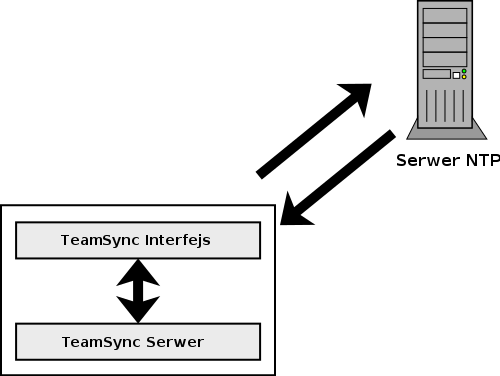
\includegraphics[width=230pt]{figures/architecturentp.png}
  \end{center}
  \caption{Komunikacja systemu \emph{TeamSync} z serwerem NTP.}
\end{figure}

Istnienie możliwości zamieszczania komentarzy przez użytkowników w dowolnej chwili działania systemu \emph{TeamSync} oraz konieczność zachowania informacji o czasie wprowadzania wypowiedzi są źródłami kilku problemów. Chcąc umożliwić rzetelne --- nie tylko co do treści, ale również co do czasu zamieszczenia komentarza --- dzielenie się swoimi opiniami przez użytkowników, należało uniknąć w systemie dwóch nastepujących przeszkód:

\begin{itemize}[noitemsep]
  \item nie ma pewności, że na każdym z węzłów jest ten sam czas systemowy, z którego użytkownik pobierałby znacznik czasowy podczas umieszczania komentarza. Jeśli różnica między czasami zamieszczanych komentarzy byłaby większa niż kilka minut, wyświetlane wypowiedzi często byłyby przedstawiane w nieprawidłowej kolejności. Komentarze napisane później (według czasu rzeczywistego) --- w wyniku różnic czasów systemowych na węzłach --- mogłyby zostać umieszczone w sieci jako napisane wcześniej niż w rzeczywistości,
  
  \item nie ma gwarancji, że wszystkie węzły w jednolity sposób będą wprowadzać znaczniki czasowe do systemu --- problem użytej przez nich jednostki oraz formatu.
\end{itemize}

\emph{Serwer NTP} \cite{ntp}, od którego użytkownicy pobierają znaczniki czasowe podczas zamieszczania komentarzy, pełni rolę neutralnego arbitra i zarazem stanowi rozwiązanie dwóch powyższych zastrzeżeń. Otrzymywanie znaczników czasowych z tego samego dla wszystkich użytkowników, neutralnego źródła jest kluczowym punktem w algorytmie dodawania nowych wypowiedzi --- w przypadku jego braku, użytkownicy mogliby wprowadzać do sieci fałszywe dane.

Potrzeba zachowania jednolitego formatu oraz jednostki znacznika czasowego wynika z konieczności zapewnienia unikalności nazw plików zawierających dane z komentarzami. Bez dostępu do serwera NTP użytkownik nie ma możliwości napisać wypowiedzi w żadnym z wątków, ponieważ narażałoby to system na generowanie konfliktów (np. poprzez dwukrotne uzyskanie tego samego znacznika czasowego przy dodaniu komentarza).

Zapytanie wysyłane jest do serwera NTP \emph{zawsze}, gdy użytkownik umieści treść komentarza (lub nowego wątku) w interfejsie graficznym i zatwierdzi jego dodanie. W odpowiedzi serwer NTP odsyła wiele wartości takich jak: znacznik czasowy, przesunięcie, precyzja, wersja protokołu itd. Najważniejszym z nich (i jedynym użytym w systemie) jest sam znacznik czasowy.

Znacznikiem czasowym, który użytkownicy otrzymują w odpowiedzi jest skoordynowanym czasem uniwersalnym (\emph{UTC --- Universal Coordinated Time}) w postaci liczby całkowitej zawierającą sekundy.
\chapter{Ogólne działanie systemu i konfiguracja}

Jak zostało napisane w sekcji \ref{teamsyncarch}, użytkownicy nie wymieniają ze sobą informacji poprzez komunikaty, lecz poprzez umieszczanie odpowiednio zainicjowanych i umieszczonych plików. Aby lepiej zrozumieć sposoby zamieszczania komentarzy, opisano w poniższych sekcjach jaką strukturę ma synchronizowany katalog, jak system jest skonfigurowany oraz jak rekompensowane są wady spowodowane przez architekturę systemu.

\section{Struktura katalogów}

\label{directorystructure}

Podczas tworzenia synchronizowanego folderu użytkownik może dołączyć do istniejącego folderu (założonego przez innego użytkownika) lub zainicjować własny. W obydwóch przypadkach uwspólniany folder musi być pusty --- wymaganie to jest powielone z aplikacji BitTorrent Sync.

Aby ułatwić i ujednoznacznić opis implementacji zastosowano następujące terminy i nazwy zmiennych:

\begin{description}[noitemsep]
 \item[właściciel] --- użytkownik, który stworzył folder i rozdysponował klucze (\emph{secrets}) do pozostałych użytkowników,
 
 \item[\textbf{[root]}] --- ścieżka będąca bezwzględną lokalizacją synchronizowanego katalogu w systemie operacyjnym użytkownika.
\end{description}

Podczas inicjowania nowego (a więc również pustego) folderu przez właściciela tworzone są wewnątrz niego dodatkowe katalogi:


\begin{verbatim}
                              [root]/
                                  .sync/
                                  .Users/
                                  .Comments/
\end{verbatim}

Katalog \emph{.sync} tworzony jest przez aplikację BitTorrent Sync i domyślnie jest ukryty. Znajduje się w nim archiwum oraz pliki niezbędne do poprawnego działania synchronizacji folderu. Usunięcie katalogu \emph{.sync} skutkuje pełnym zanikiem funkcjonalności synchronizacji i wystąpieniem błędu. Pełna struktura katalogu \emph{.sync} wygląda następująco:

\begin{verbatim}
                    .sync/
                        Archive/
                            [ lista plików w archiwum ]
                        ID
                        IgnoreList
                        StreamsList
\end{verbatim}

\begin{itemize}[noitemsep]
 \item folder \emph{Archive} zawiera wersje plików, które zostały usunięte/zmodyfikowane podczas synchronizacji,
 
 \item plik \emph{ID} reprezentuje identyfikator folderu, dzięki któremu możliwe jest znalezienie innych użytkowników lub urządzeń uwspólniających ten sam folder przez aplikację BitTorrent Sync,
 
 \item plik \emph{IgnoreList} jest plikiem tekstowym, wewnątrz którego zawarta jest lista plików pomijanych podczas synchronizacji (wspierane są znaki: ,,*'' --- oznaczający dowolny ciąg znaków  oraz ,,?'' --- oznaczający jeden dowolny znak),
 
 \item plik \emph{StreamsList} w odróżnieniu od \emph{IgnoreList} zawiera listę plików (obsługującą rozszerzone atrybuty plików), które będą synchronizowane (tzw. ,,white list'').
\end{itemize}


Pozostałe dwa foldery (\emph{.Comments} oraz \emph{.Users}) tworzone są przez aplikację zaimplementowaną w ramach niniejszej pracy i podobnie jak katalog \emph{.sync} są katalogami ukrytymi. Ewentualne usunięcie któregoś z tych katalogów będzie skutkować niepoprawnym działaniem aplikacji: w przypadku zniknięcia folderu \emph{.Comments} znikną wszystkie komentarze, a w przypadku \emph{.Users} aplikacja nie będzie mogła rozpoznać użytkowników piszących komentarze i współdzielących folder, co będzie skutkować błędami.

Wszystkie usunięte pliki z synchronizowanego folderu są utrzymywane w archiwum wewnątrz tego folderu, więc możliwe jest ,,ręczne'' przekopiowanie utraconych danych z powrotem w przypadku przypadkowego (lub celowego) ich usunięcia. Czas, jaki mają użytkownicy na przywrócenie usuniętych danych to 30 dni --- po tym czasie dane sa usuwane bezpowrotnie Do ewentualnej rozbudowy aplikacji można dołączyć automatyczne odtwarzanie nie tylko całych usuniętych struktur \emph{.Users} oraz \emph{.Comments}, ale również usuniętych plików, do których odnosiły się niektóre wątki w systemie.

\subsection{Katalog \emph{.Users}}

Podczas dołączania użytkownika do synchronizowanego folderu umieszcza on w katalogu \emph{.Users} plik tekstowy o rozszerzeniu JSON, wewnątrz którego zapisuje słownik z danymi o sobie. Tworzony jest słownik o kluczach \emph{uid} oraz \emph{identity}, gdzie wartość \emph{uid} to identyfikator użytkownika, a \emph{identity} to nazwa użytkownika widziana przez innych użytkowników w aplikacji. Zainicjowany słownik zostaje zapisany do katalogu \emph{.Users} pod nazwą \texttt{<UID użytkownika>.json}.

Taki sposób rozwiązania problemu zapisywania i wymiany danych o użytkownikach został wprowadzony ze względu na perspektywy rozwoju aplikacji. Utworzono fundamenty, które mogą być wygodnie i efektywnie rozbudowywane w kolejnych wersjach aplikacji.

Rozwiązaniem łatwiejszym byłby jeden plik z listą wszystkich użytkowników, w którym podczas dołączania do folderu kolejni użytkownicy wprowadzaliby dane na swój temat. Niestety wszelkie modyfikacje plików grożą możliwością wystąpienia konfliktu podczas równoczesnego wprowadzania zmian. Zrezygnowano więc z takiego rozwiązania na rzecz tworzenia nowych plików zamiast edytowania już istniejących.

Przykładowa struktura wewnątrz folderu \emph{.Users}:

\begin{minipage}{\linewidth}
\vspace{1em}
\begin{verbatim}
              .Users/
                  2HI7KMNQWPONLKFORRWXGOTIZSHBGFIH.json
                  2SAFDSBCXGFD765GDFS4GFDS35FDSBVB.json
                  3REW54GFDS6578FDSGDF5BSH652F2B34.json
\end{verbatim}
\vspace{1em}
\end{minipage}

Zawartość pliku \texttt{2HI7KMNQWPONLKFORRWXGOTIZSHBGFIH.json} pochodzącego z katalogu \emph{.Users}:

\begin{figure}[htb]
  \begin{verbatim}
                {
                    "uid": "2HI7KRUNSSONIUJKMRWXGOTIZSHBGFIH", 
                    "identity": "Filip Rachwalak"
                }
  \end{verbatim}
  \caption{Przykładowy plik użytkownika.}
\end{figure}

W przypadku takiej zawartości folderu \emph{.Users} system TeamSync wyświetli w graficznym interfejsie trzech użytkowników. Biorąc pod uwagę, że zawartość pliku \texttt{2HI7KMNQWPONLKFORRWXGOTIZSHBGFIH.json} jest identyczna z przedstawioną powyżej, wyświetlaną nazwą jednego z użytkowników będzie ,,Filip Rachwalak''.

\subsection{Katalog \emph{.Comments}}

W przeciwieństwie do katalogu \emph{.Users} --- którego struktura jest płaska, a elementy tworzą listę --- folder \emph{.Comments} jest znacznie bardziej złożony. W miarę przybywania wątków katalog zwiększa swoją objętość zarówno wszerz jak i wgłąb, ponieważ wewnątrz niego odzwierciedlona jest drzewiasta struktura synchronizowanego katalogu. Dla łatwiejszego zrozumienia przyjmijmy następujący folder, który dwóch użytkowników współdzieli ze sobą:

\begin{minipage}{\linewidth}
\vspace{1em}
\begin{verbatim}
              [root]/
                  .sync/
                      [ pliki aplikacji BitTorrent Sync ]
                  .Users/
                      2HI7KMNQWPONLKFORRWXGOTIZSHBGFIH.json
                      2SAFDSBCXGFD765GDFS4GFDS35FDSBVB.json
                  .Comments/
                  test1/
                      test2/
                          eee.txt
                      ccc.txt
                      ddd.txt
                  aaa.txt
                  bbb.txt
\end{verbatim}
\vspace{1em}
\end{minipage}

Jeśli użytkownik utworzyłby wątek dotyczący pliku \emph{[root]/aaa.txt}, aplikacja umieściłaby folder z wątkiem na pierwszym poziomie katalogu \emph{.Comments} zgodnie z lokalizacją pliku w głównym folderze. Natomiast jeśli użytkownik zacząłby wątek o plik \emph{[root]/test1/ccc.txt}, program stworzyłby dodatkowy folder wewnątrz \emph{.Comments} o nazwie \emph{test1} i w nim umieściłby folder z nowym wątkiem.

Aby łatwiej było zrozumieć tworzenie nowych folderów z wątkami, załóżmy, że użytkownik utworzył trzy wątki o trzech plikach: \emph{aaa.txt} w głównej lokalizacji, \emph{ccc.txt} wewnątrz katalogu \emph{test1}, oraz \emph{eee.txt} wewnątrz katalogu \emph{test2}. Wówczas struktura folderu \emph{.Comments} wyglądałaby następująco:

\begin{minipage}{\linewidth}
\vspace{1em}
\begin{verbatim}
                  .Comments/
                      test1/
                          test2/
                              wątek_o_eee/
                                  [ pliki z komentarzami ]
                          wątek_o_ccc/
                              [ pliki z komentarzami ]
                      wątek_o_aaa/
                          [ pliki z komentarzami ]
\end{verbatim}
\vspace{1em}
\end{minipage}

Łatwo zauważyć, że w miarę przybywania wątków, struktura folderu rozrasta się i zbliża do struktury głównego folderu (oczywiście z pominięciem trzech ukrytych, dodatkowych katalogów oraz folderów przechowujących wątki). Przechowywanie komentarzy w ten sposób ma niestety swoją wadę --- wrażliwość na przenoszenie danych w obrębie uwspólnionego katalogu. Wyeliminowanie tego ograniczenia mogłoby należeć do najbliższych ulepszeń aplikacji w przyszłości.

\section{Pliki konfiguracyjne}

Ustawienia aplikacji, identyfikator użytkownika, adres serwera BitTorrent Sync API --- wszystkie niezbędne informacje do poprawnego działania systemu TeamSync, tworzonego w ramach niniejszej pracy magisterskiej, zawarte są wewnątrz plików konfiguracyjnych w formacie JSON (pliki \texttt{config.json} oraz \texttt{btsyncconfig.json}). Zlokalizowane są one wewnątrz głównego katalogu aplikacji --- istnieje więc tylko jedna instancja każdego z plików i jest globalna w skali aplikacji (nie jest powielana w każdym synchronizowanym folderze).

Podczas uruchamiania aplikacji sprawdzana jest obecność tych plików. W przypadku ich obecności pobierane są z nich ustawienia i wykorzystywane w programie. Wszelka samodzielna modyfikacja tych plików np. poprzez edycję za pomocą dowolnego narzędzia do modyfikacji tekstu, może zakłócić działanie aplikacji ze względu na np. kodowanie znaków lub składnię formatu JSON. Jeśli aplikacja nie znajdzie któregoś z dwóch plików (np. podczas pierwszego uruchomienia programu), zainicjuje je i wypełni domyślnymi ustawieniami. Szczegóły przydzielanych ustawień oraz ich lista zostaną dokładnie omówione w następnych podrozdziałach.

\subsection{Konfiguracja BitTorrent Sync}

\label{configbtsync}

Pierwszym z dwóch plików z ustawieniami jest \texttt{btsyncconf.json} zawierający informacje potrzebne do komunikacji programu Team Sync z aplikacją BitTorrent Sync. Podczas uruchamiania zaimplementowanej aplikacji inicjowany jest również BitTorrent Sync z przełącznikiem \texttt{--config} wskazującym na plik z ustawieniami.

Aby możliwa była komunikacja z systemem BitTorrent Sync, konieczna jest znajomość adresu wraz z numerem portu, na którym API będzie nasłuchiwać i na który system TeamSync będzie wysyłał żądania. W pliku konfiguracyjnym znajdują się również pola niezbędne podczas autoryzacji żądania: \texttt{login} oraz \texttt{password}. Istnieje możliwość zablokowania domyślnego interfejsu wystawianego przez aplikację BitTorrent Sync, który nie jest potrzebny do poprawnego działania całości i został domyślnie zablokowany. Ostatnie dwa elementy obecne w pliku z ustawieniami to: \texttt{storage\_path} oraz \texttt{api\_key}.

Wartość pola \texttt{api\_key} jest ciągiem znaków, który jest generowany przez twórców BitTorrent Sync i wydawany na prośbę deweloperów chcących testować API lub wytwarzać własne oprogramowanie z jego wykorzystaniem (z zastrzeżeniem o niekomercyjnym przeznaczeniu oprogramowania). Jeśli plik konfiguracyjny aplikacji BitTorrent Sync odczyta plik konfiguracyjny i nie będzie miał wypełnionego tego pola (lub będzie wypełnione niepoprawnym kluczem), API nie będzie odpowiadało na żądania.

\texttt{storage\_path} jest ścieżką do katalogu ustawianą przez użytkownika, w którym będą przechowywane informacje potrzebne aplikacji BitTorrent Sync:

\begin{itemize}[noitemsep]
  \item pliki potrzebne do uruchomienia graficznego interfejsu aplikacji BitTorrent Sync,
  
  \item pliki tekstowe logów rejestrujące powstawanie nowych torrentów i nadawanie im znaczników czasowych,
  
  \item plik ustawień,
  
  \item plik historii,
  
  \item plik logów rejestrujący wszelkie zdarzenia dotyczące synchronizacji (w zależności od użytych jej sposobów),
  
  \item plik przechowujący identyfikator procesu aplikacji BitTorrent Sync, użyteczny podczas wyłączania programu TeamSync.
\end{itemize}

Poniżej umieszczono przykładowy plik konfiguracyjny \texttt{btsyncconfig.json}. Z wyjątkiem \texttt{api\_key} oraz \texttt{storage\_path} identyczny plik jest tworzony podczas pierwszego uruchomienia aplikacji TeamSync.

\begin{figure}[htb]
  \begin{verbatim}
  {
      "use_gui": false, 
      "webui": {
          "api_key": "<<ciąg znaków wg. wyrażenia regularnego [A-Z0-9]{136}>>", 
          "login": "team", 
          "password": "sync", 
          "listen": "127.0.0.1:8787"
      }, 
      "storage_path": "/home/user/teamsync/.btsync-files"
  }
  \end{verbatim}
  \caption{Przykładowy plik konfiguracyjny \texttt{btsyncconfig.json}.}
\end{figure}

Interpretacja przykładowego pliku konfiguracyjnego jest następująca: BitTorrent Sync nie będzie miał dostępnego oryginalnego interfejsu graficznego, natomiast wystawione API będzie odbierało żądania na adresie \texttt{127.0.0.1} oraz porcie \texttt{8787}. Aby polecenia wewnątrz zapytań zostały wykonane, wewnątrz nich muszą zawierać się dane uwierzytelniające \texttt{team} jako \emph{login} oraz \texttt{sync} jako \emph{password}. Ścieżka zapisu plików potrzebnych dla aplikacji BitTorrent Sync to \texttt{/home/user/\-teamsync/.btsync-files}.

\subsection{Konfiguracja TeamSync}

\label{configteamsync}

Plik \texttt{config.json}, wewnątrz którego zapisana jest konfiguracja systemu \emph{TeamSync}, zawiera zarówno informacje dotyczące lokalizacji aplikacji, adresu serwera NTP, zapisanych tożsamości użytkownika w różnych folderach, jak i danych ułatwiających korzystanie z programu np. zapamiętane ostatnie ustawienia sortowania wątków. Podobnie jak plik \texttt{btsyncconfig.json} jest on wczytywany na początku działania programu lub tworzony jest nowy, z domyślnymi ustawieniami w przypadku jego nieobecności wewnątrz folderu przechowującego aplikację.

Poniżej opisane zostaną pola konfiguracji --- wraz z wartościami, jakie mogą przyjmować --- podzielone na grupy odpowiadające powierzonym im funkcjom.

\subsubsection*{Ustawienia ogólne}

\begin{itemize}[noitemsep]
  \item \emph{uid} --- identyfikator użytkownika generowany przez BitTorrent API. W celu uzyskania identyfikatora podczas tworzenia konfiguracji wysyłane jest żądanie \texttt{get\_secrets} (podrozdział \ref{getsecrets}, metoda \emph{get\_secrets}) zwracające trzy ciągi losowych znaków --- jeden z wyników użyty jest jako wartość pola \texttt{uid},
  
  \item \emph{operating\_system} --- system operacyjny sprawdzany przez program przy tworzeniu konfiguracji podczas pierwszego uruchomienia,
  
  \item \emph{btsync\_server\_address} --- adres oraz port, na którym BitTorrent Sync API nasłuchuje żądań od aplikacji TeamSync. Podobnie jak w pliku konfiguracyjnym systemu BitTorrent Sync, ustawione domyślnie na \texttt{127.0.0.1:8787},
  
  \item \emph{identities} --- wartość tego pola ma strukturę słownika, który w kluczach przechowuje \texttt{secret} folderu synchronizowanego przez użytkownika, a w wartości tzw. ,,tożsamość'', czyli nazwa, którą użytkownik wpisuje służąca do identyfikacji użytkowników między sobą wewnątrz folderu.
\end{itemize}

\subsubsection*{NTP}

Zawarte w tej grupie ustawienia są potrzebne do komunikacji z serwerem NTP, z którego korzysta aplikacja podczas umieszczania komentarzy.

\begin{itemize}[noitemsep]
  \item \emph{ntp\_server\_name} --- nazwa domenowa serwera NTP, z którego użytkownik chce korzystać. Domyślnie przyjmowana jest wartość \texttt{pl.pool.ntp.org} ze względu na lokalizację,
  \item \emph{ntp\_server\_version} --- wersja serwera NTP, domyślnie wersja $3$ (wersja $4$ w momencie pisania pracy jest w trakcie implementacji).
\end{itemize}

W przypadku dalszego rozwoju aplikacji możliwa będzie zmiana tych wartości przez użytkownika, co umożliwi wygodne korzystanie z aplikacji w innej strefie czasowej lub w nowszej wersji serwera NTP.

\subsubsection*{Ułatwienia dostępu}

Grupa ustawień, której jedynym zadaniem jest przyspieszanie pracy serwera aplikacji, aby nie było konieczne każdorazowe sprawdzanie ścieżki katalogu, wewnątrz którego znajduje się aplikacja.

\begin{itemize}[noitemsep]
  \item \emph{application\_path} --- bezwzględna ścieżka, w której znajduje się główna część aplikacji,
  \item \emph{btsync\_exe\_file} --- bezwzględna lokalizacja wykonywalnego pliku aplikacji BitTorrent Sync,
  \item \emph{btsync\_conf\_file} --- bezwzględna lokalizacja pliku z konfiguracją aplikacji BitTorrent Sync.
\end{itemize}

Zapisywanie powyższych ścieżek do pliku konfiguracyjnego wpływa również na przejrzystość kodu, ponieważ częste ich używanie w formie wymagającej każdorazowej konkatenacji odpowiednich łańcuchów znakowych z dodatkowymi lokalizacjami byłoby uciążliwe dla programisty. Znacznie łatwiej i przejrzyściej czytać powyższe dane z pliku i przechowywać je w pamięci programu.

\subsubsection*{Ustawienia interfejsu graficznego}

Ustawienia z tej grupy stworzone zostały z myślą o przyszłym rozwoju aplikacji w sferze graficznego interfejsu użytkownika. Obecnie nie ma możliwości ich zmiany, użytkownik musi pozostać przy ustawieniach domyślnych.

\begin{itemize}[noitemsep]
  \item \emph{comments\_date\_format} --- format daty wpisu, który użytkownik będzie mógł zmieniać w oparciu o kilka objaśnionych reguł. Wartość jest ustawiona domyślnie na \texttt{HH:mm - d.MM.yyyy}, a przykładowy wynik takiego formatowania to \texttt{12:34 - 7.04.2015},
  \item \emph{threadsorting1} --- pole, którego wartość zapamiętuje ,,ulubiony'' typ sortowania wątków. Poniżej znajduje się lista możliwych wartości z ich objaśnieniem:
  
  \begin{itemize}[noitemsep]
    \item \emph{name} --- sortowanie według nazwy wątku,
    \item \emph{timestamp} --- sortowanie według czasu rozpoczęcia wątku,
    \item \emph{numberofcomments} --- sortowanie według ilości komentarzy w wątku,
    \item \emph{lastcomment} --- sortowanie według najświeższej odpowiedzi.
  \end{itemize}
  
  \item \emph{threadsorting2} --- kierunek sortowania, możliwe wartości to: \emph{ascending} oraz \emph{descending}, domyslnie \emph{ascending}.
\end{itemize}

Wewnątrz tej grupy ustawień w ewentualnym przyszłym rozwoju aplikacji będą umieszczane dane związane np. z kolorem czcionki albo ramek, w których wyświetlane są komentarze.

\subsubsection*{Przykładowy plik konfiguracyjny}

Poniżej przestawiony zostanie przykładowy plik konfiguracyjny wypełniony domyslnymi wartościami podczas pierwszego tworzenia. Aby urzeczywistnić przykład do słownika \emph{identities} zostaną dodane przykładowe wpisy.

\begin{figure}[htb]
  \begin{verbatim}
          {
              "uid": "2HI7KRUNSSONIUJKMRWXGOTIZSHBGFIH",
              "operating_system": "Linux", 
              "btsync_server_address": "127.0.0.1:8787", 
              "identities": {
                  "AKO6XM5HJZJ2DFAG2NJ7T4PVAIA4U25XQ": "Filip Rachwalak", 
                  "AQXKJKAC6XNJKNLE2YW6EOMCCBHG2UBUL": "Jan Iksiński"
              }, 
    
              "ntp_server_name": "pl.pool.ntp.org", 
              "ntp_server_version": 3, 

              "application_path": "/home/user/teamsync",           
              "btsync_exe_file": "/home/user/teamsync/btsync",
              "btsync_conf_file": "/home/user/teamsync/btsyncconfig.json",

              "commentsDateFormat": "HH:mm - d.MM.yyyy", 
              "threadsorting1": "timestamp", 
              "threadsorting2": "ascending", 
          }
  \end{verbatim}
  \caption{Przykładowy plik konfiguracyjny \texttt{config.json}.}
\end{figure}

Według powyższej konfiguracji użytkownik posiada identyfikator \texttt{2HI7KRUN\-SSONIUJKM\-RWXGOTIZ\-SHBGFIH} i pracuje na systemie operacyjnym \texttt{Linux}. Adres BitTorrent Sync API, na który wysyłane będą żądania to domyślny adres \texttt{127.0.0.1:8787}. Użytkownik ma dwa współdzielone foldery: pierwszy o łańcuchu \emph{secret} \texttt{AKO6XM5H\-JZJ2DFAG2\-NJ7T4PVAI\-A4U25XQ}, wewnątrz którego inni identyfikują go pod nazwą \texttt{Filip \-Rachwalak} i drugi o łańcuchu \emph{secret} \texttt{AQXKJKAC\-6XNJKNLE2\-YW6EOMCC\-BHG2UBUL} gdzie tą nazwą jest \texttt{Jan \-Iksiński}.

Ustawienia serwera \texttt{NTP} są domyślne dla Polski i dla aktualnej wersji usługi. Aplikacja TeamSync została zainstalowana wewnątrz lokalizacji \texttt{/home\-/user\-/teamsync}, o czym świadczy właściwość \texttt{application\_\-path}. Bezwzględne ścieżki pliku wykonywalnego oraz konfiguracyjnego aplikacji BitTorrent Sync to odpowiednio \texttt{/home/user/\-teamsync/btsync} oraz \texttt{/home/user/\-teamsync/\-btsyncconfig.json}.

Ustawiony format czasu zamieszczenia komentarza wyświetlany w intefejse graficznym razem z nim to \texttt{HH:mm - d.MM.yyyy}. Oznacza to, że przykładowa godzina będzie wyświetlana w następujący sposób: \texttt{22:12}, a data: \texttt{7.11.2014}. Oddzielać je będzie myślnik, co --- dla wymienionej wyżej przykładowej daty oraz godziny --- da wyjściowy efekt: \texttt{22:12 - 7.11.2014}. Ustawienia dotyczące sortowania skutkować będą zmianą kolejności wątków podczas wyświetlania ich listy według czasu powstania wątku (\texttt{timestamp}) w porządku rosnącym (\texttt{ascending}).

\section{Spójność komentarzy w wątku}

\label{consistencies}

Z uwagi na rozproszoną architekturę aplikacji TeamSync, należy zwrócić uwagę na możliwość logicznego zaburzenia przepływu dyskusji. Nie ma pewności, że wszyscy użytkownicy w każdej chwili będą mieli ,,aktualną'' wersję rozmowy. Może zajść sytuacja, w której użytkownik \texttt{A} wypowie się na pewien temat widząc tylko jeden komentarz w wątku (początkowy), podczas gdy w rzeczywistości już inni użytkownicy się wypowiedzieli, lecz użytkownik \texttt{A} nie zdążył uspójnić z nimi nowych danych. Wówczas może zdarzyć sie sytuacja, w której użytkownicy czytający wypowiedź użytkownika \texttt{A} --- po ostatecznym, całkowitym uspójnieniu danych --- będą się zastanawiać nad jej logicznym sensem.

Dla lepszego opisania problemu w dalszej części sekcji rozważana będzie następująca sytuacja: w systemie istnieje wątek dotyczący pewnego zdjęcia z jednym komentarzem o treści: ,,\textit{Zdjęcie zrobione w Afryce podczas zachodu słońca u stóp Kilimandżaro}'' (wszyscy użytkownicy w systemie posiadają swoją lokalną kopię tego komentarza). Dodatkowo istnieje trzech użytkowników: \texttt{A}, \texttt{B} oraz \texttt{C}, którzy będą wypowiadać się na temat tego pliku. Jednak działają wewnątrz systemu rozproszonego, więc można założyć, że częsta będzie sytuacja, w której nieobecny będzie jeden lub kilku z węzłów współdzielących folder. Niech użytkownik \texttt{C} będzie nieobecny w systemie (do tej pory wszyscy użytkownicy --- łącznie z użytkownikiem \texttt{C} --- mają poprawnie zsynchronizowany wątek o zdjęciu --- mogą odczytać pierwszy komentarz). Wówczas --- podczas nieobecności węzła \texttt{C} --- tak mogłaby wyglądać krótka konwersacja użytkowników \texttt{A} oraz \texttt{B}:

\vspace{5px}
\begin{center}
\begin{tabular}{c | c | c | c}
 \textbf{Autor} & \textbf{Treść komentarza} & \textbf{Czas dodania} & \textbf{Odczytane przez \texttt{C}}\\
 \hline
 \texttt{A} & To zdjęcie bardzo mi się podoba! & 20:35:00 & --- \\
 \texttt{B} & Faktycznie, ładne zdjęcie & 20:38:00 & ---
\end{tabular}
\end{center}
\vspace{5px}

Komentarze przechowywane są w plikach, w których zawarta jest treść (odpowiadająca kolumnie \textbf{Treść komentarza}), autor (kolumna \textbf{Autor}) oraz znacznik czasowy (kolumnie \textbf{Czas dodania}). Kolumna \textbf{Odczytane przez \texttt{C}} jest odzwierciedleniem zmiennej \emph{readby} dla użytkownika \texttt{C} wewnątrz komentarza (dokładny opis mechanizmu \emph{readby} znajduje się w sekcji \ref{archcomments}). Widać, że użytkownicy napisali po jednym komentarzu o godzinie 20:35 oraz 20:38. Wartości w ostatniej kolumnie --- przechowującej czas przeczytania komentarzy przez użytkownika \texttt{C} --- nie są wprowadzone, ponieważ użytkownik \texttt{C} nie zsynchronizował jeszcze folderu z komentarzami z użytkownikami \texttt{A} oraz \texttt{B}, co oznacza, że nie przeczytał ich wypowiedzi.

Następnie obydwaj użytkownicy rozłączają się z sieci. Po chwili niepozwalającej na ewentualną komunikację z obydwoma użytkownikami, (np. o godzinie 21:20) użytkownik \texttt{C} uruchamia aplikację TeamSync i umieszcza swój komentarz: ,,\emph{Nie wiem jak Wam, ale mi się podoba!}'' (według jego najlepszej wiedzy jest pierwszym, który odpowiada na wypowiedź inicjującą wątek). Po jakimś czasie (około godziny 22:00) do systemu podłączają się dwaj pozostali użytkownicy i wszyscy trzej uspójniają wszystkie dane. Okazuje się, że kolejność umieszczenia wypowiedzi wewnątrz wątku jest następująca:

\vspace{5px}
\begin{center}
\begin{tabular}{c | c | c | c}
 \textbf{Autor} & \textbf{Treść komentarza} & \textbf{Czas dodania} & \textbf{Odczytane przez \texttt{C}}\\
 \hline
 \texttt{A} & To zdjęcie bardzo mi się podoba! & 20:35:00 & 22:00:14 \\
 \texttt{B} & Faktycznie, ładne zdjęcie & 20:38:00 & 22:00:15 \\
 \texttt{C} & Nie wiem jak Wam, ale mi się podoba! & 21:20:00 & 21:20:13
\end{tabular}
\end{center}
\vspace{5px}

Z punktu widzenia użytkowników \texttt{A} i \texttt{B}, logika wypowiedzi użytkownika \texttt{C} jest mocno zaburzona. Jest to konsekwencja rozproszonej architektury systemu (systemu BitTorrent Sync odpowiedzialnego za transport danych), której \emph{nie ma możliwości} zniwelować bez implementacji dodatkowych algorytmów rozproszonych, lub włączania w architekturę nieustannie dostępnego węzła, synchronizującego wszystkie dane na bieżąco w czasie rzeczywistym. Wówczas można już mówić o pewnej centralizacji systemu, czego w ramach niniejszej pracy chciano uniknąć.

W systemie TeamSync zaimplementowano mechanizm, dzięki któremu można ,,usprawiedliwiać'' użytkowników, których logika i sens komentarzy bardzo lub tylko nieznacznie odbiegają od norm, lub którzy powielają wypisane wcześniej kwestie. Problem rozwiązano poprzez możliwość ustawienia takiego sposobu szeregowania dyskusji, aby każdy z użytkowników mógł przeczytać ją w takiej kolejności, w jakiej przeczytał ją autor wątpliwego komentarza. Kontynuując przykład ze zdjęciem z Afryki, jeśli użytkownik \texttt{A} chciałby odczytać dyskusję tak, jak odczytał ją użytkownik \texttt{C} musiałby zmienić w interfejsie graficznym spójność na ,,spójność według użytkownika \texttt{C}'' (dokładny opis funkcjonalności znajduje się w dodatku, w sekcji \ref{gui}). Wówczas zobaczyłby następującą kolejność komentarzy:

\vspace{5px}
\begin{center}
\begin{tabular}{c | c | c | c}
 \textbf{Autor} & \textbf{Treść komentarza} & \textbf{Czas dodania} & \textbf{Odczytane przez \texttt{C}}\\
 \hline
 \texttt{C} & Nie wiem jak Wam, ale mi się podoba! & 21:20:00 & 21:20:13 \\
 \texttt{A} & To zdjęcie bardzo mi się podoba! & 20:35:00 & 22:00:14 \\
 \texttt{B} & Faktycznie, ładne zdjęcie & 20:38:00 & 22:00:15
\end{tabular}
\end{center}
\vspace{5px}

Po obejrzeniu dyskusji w powyższej kolejności użytkownicy mogą w większym stopniu zrozumieć się nawzajem i uniknąć nieporozumień wynikających nie z ich błędu, lecz z założeń architektonicznych systemu. Co prawda funkcjonalność zmiany punktu odniesienia w czytaniu wątków w pewnym stopniu rekompensuje wady architektury, natomiast nie niweluje ich całkowicie, z czym jednak użytkownicy systemu rozproszonego powinni się liczyć.
\chapter{Implementacja}

\section{Zastosowane technologie}

Wybór technologii użytych w implementacji został podyktowany jej architekturą --- interfejs użytkownika dostępny jest tylko i wyłącznie w przeglądarce internetowej, z tego powodu wybrane przez autora i opisane poniżej narzędzia są kojarzone jedynie w obszarze technologii internetowych. Interfejs graficzny wywarł niemały wpływ na wybór narzędzi, z uwagi na fakt, że osoba korzystająca z aplikacji powinna w łatwy i intuicyjny sposób:

\begin{itemize}[noitemsep]
  \item poruszać się po katalogach, plikach oraz wątkach,
  \item wyszukiwać wątki, komentarze lub pojedyncze słowa wewnątrz nich,
  \item wydzielić te wątki, które najbardziej interesują użytkownika,
  \item przeglądać statystyki dotyczące wpisywanych komentarzy.
\end{itemize}

Narzędzie, które zostało wybrane do realizacji tych zadań to AngularJS \cite{angular} --- technologia ułatwiająca kontrolę nad elementami interfejsu, stworzona w języku JavaScript. Jednakże, aby cały system prawidłowo i sprawnie działał, potrzebna była również technologia, która umożliwia przekazanie do interfejsu danych w odpowiedniej formie, pobranie z niego zadań wyznaczonych przez użytkownika i odpowiednie ich zrealizowanie. Do tych celów użyto języka Python \cite{python} wraz z narzędziem o nazwie Django \cite{django} do implementacji aplikacji internetowych. Połączenie Python/Django oraz AngularJS okazało się wystarczające do stworzenia aplikacji --- poza nimi użyte zostały wyłącznie skrypty odpowiadające za wygląd interfejsu.

\subsection*{AngularJS}

AngularJS jest otwartą biblioteką języka JavaScript, która została stworzona w 2009 roku i obecnie jest wspierana przez firmę Google. Najważniejszą funkcją narzędzia jest dwukierunkowe wiązanie danych (tzw. ,,emph{two-way data binding}''), które wyjątkowo łatwo obsługuje się wewnątrz szablonów HTML --- za ich pomocą zmiany wewnątrz modelu są natychmiast odzwierciedlone w interfejsie i na odwrót: elementy wprowadzone bądź zmienione przez użytkownika natychmiastowo znajdują odzwierciedlenie w modelu.

Biblioteka korzysta z wzorca MVC (Model-View Controller), aby ułatwić nie tylko implementację, ale również testowanie tworzonego systemu. AngularJS umożliwia bardzo łatwe zarządzanie dynamiczną treścią poprzez wspomniane wcześniej szablony i dodatkowe komendy wewnątrz szablonów. Dynamika aplikacji zaimplementowanej w niniejszej pracy była głównym wyzwaniem podczas jej tworzenia, a biblioteka AngularJS znacząco wpłynęła zarówno na poprawność, jak i objętość kodu.

\subsection*{Django}

O ile AngularJS został wykorzystany w znacznej mierze, o tyle stopień wykorzystania funkcjonalności Django został zredukowany do minimum. Biblioteka Django jest biblioteką do kompleksowego budowania stron internetowych w dowolnych architekturach (np. REST \cite{rest}), stworzoną, by jak najbardziej automatyzować kod i jak najszybciej --- a zarazem jak najprościej --- tworzyć skomplikowane serwisy. Narzędzie użyte zostało do implementacji z uwagi na prostotę i możliwości testowania, debugowania oraz możliwości rozbudowania zaimplementowanej aplikacji o dodatkowe rozwiązania.

Biblioteka Django powstała w 2003 roku, stworzona została przez programistów związanych ze środowiskiem dziennikarskim, dzięki czemu przystosowana jest do szybkiej i nieskomplikowanej pracy. Podobnie jak AngularJS pozwala (poprzez mechanizm szablonów) na łatwe i intuicyjne umieszczanie dynamicznych elementów na stronie. Wybrana została głównie ze względu na swoją prostotę oraz dodatkowe funkcjonalności ułatwiające pracę nad aplikacją np. możliwość automatycznego ponownego uruchamiania serwera podczas wprowadzania w nim zmian (co jest robione automatycznie).

\section{Komunikacja z serwerem}

Komunikacja między klientem a serwerem odbywa się poprzez zapytania \texttt{HTTP}, wewnątrz których przesyłane są dane potrzebne zarówno stronie klienta do ich wyświetlenia, jak i stronie serwera do wprowadzenia ich do systemu. Poniżej dokładnie opisane zostaną operacje wykonywane przez serwer, podzielone na grupy ze zbliżonym obszarem funkcjonalności.

\subsection{Foldery}

Operacje dostępne dla folderów w aplikacji TeamSync zostały ograniczone do dodawania ich oraz usuwania. Dodatkowe okna z ustawieniami, edycja folderów zostały przewidziane jako ewentualną dalszą rozbudowę systemu. W pracy skupiono się na pełnowartościowym korzystaniu z podstawowej funkcjonalności (synchronizacja danych oraz wprowadzanie komentarzy), co zostało spełnione bez konieczności implementacji edycji folderów.

\subsubsection*{Pobieranie listy folderów}

\begin{figure}[h!]
  \vspace{5pt}
  \begin{center}
    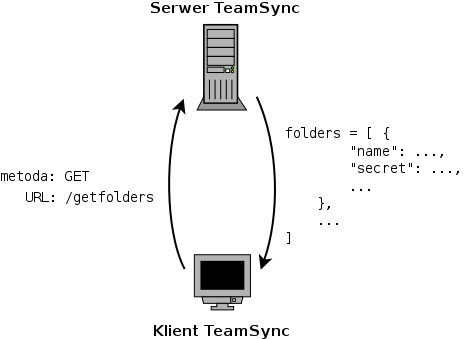
\includegraphics[width=250pt]{figures/metgetfolders.png}
  \end{center}
  \caption{Komunikacja w systemie \emph{TeamSync} podczas wywoływania metody \texttt{getfolders} --- pobieranie listy folderów.}
  \label{picmetgetfolders}
\end{figure}

Aby umożliwić użytkownikowi wybór folderu z listy synchronizowanych katalogów, aplikacja przeglądarkowa wysyła do serwera zapytanie \texttt{HTTP} za pomocą metody \texttt{GET} na adres \texttt{http://<adres oraz port serwera TeamSync>\-/getfolders}. Odpowiedź z serwera umieszczana jest wewnątrz listy \texttt{folders}, która przechowuje informacje dotyczące katalogów zapisane w formacie \texttt{JSON}.

\begin{figure}[htb!]
\label{newcommentrequest}
  \begin{verbatim}
          [
              {
                  "name": "testowy katalog", 
                  "dir": "/home/user/testowy katalog", 
              
                /* wartości mniej istotne, pobrane podczas
                   wykonywania metody get_folders takie jak: size,
                   down_speed, up_speed, error, indexing, id, type */
         
                  "secret": "A3LL43HJ257YCKMOLAD7QSEAS7U373BVO", 
                  "identity": "Filip Rachwalak", 
                  "uid": "FWZPQQKUE3JPQKWY557FERJ4SD3BSFMM", 
                  "users": [
                      {
                          "uid": "PWGGJTDPC35O43SLEKFPBPIG3NYV7PH7", 
                          "identity": "Jan Iksiński"
                      }, 
                      {
                          "uid": "FWZPQQKUE3JPQKWY557FERJ4SD3BSFMM", 
                          "identity": "Filip Rachwalak (Ty)"
                      }
                  ]
              }
          ]
  \end{verbatim}
  \caption{Przykładowa odpowiedź serwera na żądanie pobrania listy synchronizowanych folderów.}
\end{figure}

W odpowiedzi serwera znajdują się wszystkie informacje dotyczące folderów otrzymane z BitTorrent Sync API (w sekcji \ref{btsyncapiproto} znajduje się dokładne wyjaśnienie zwracanych danych przez metodę \texttt{get\_folders}) z dodatkowymi danymi:

\begin{itemize}[noitemsep]
  \item \emph{name} --- ułatwia interfejsowi wyświetlanie nazwy katalogu w liście,
  
  \item \emph{identity} oraz \emph{uid} --- tożsamość i identyfikator użytkownika,
  
  \item \emph{users} --- lista użytkowników zawierająca ich identyfikatory oraz tożsamości, potrzebna do wyświetlania wszystkich użytkowników w folderze oraz autorów komentarzy. Wartości wewnątrz tej listy są pobrany z katalogu \texttt{.Users} wewnątrz folderu współdzielonego.
\end{itemize}

W powyższym przykładzie użytkownik o identyfikatorze \texttt{FWZPQQKU\-E3JPQKWY\-557FERJ4\-SD3BSFMM} i tożsamości \texttt{Filip Rachwalak} posiada tylko jeden współdzielony folder, który dzieli z użytkownikiem \texttt{Jan Iksiński} o identyfikatorze \texttt{PWGGJTDP\-C35O43SL\-EKFPBPIG3\-NYV7PH7}. Bezpośrednia ścieżka katalogu to \texttt{/home/user/\-testowy katalog}, natomiast nazwa, jaka będzie wyświetlana na liście w przeglądarce to \texttt{testowy katalog}. \emph{Secret} folderu to \texttt{A3LL43HJ2\-57YCKMOL\-AD7QSEAS7\-U373BVO}.

\subsubsection*{Tworzenie folderu}

\begin{figure}[h!]
  \vspace{5pt}
  \begin{center}
    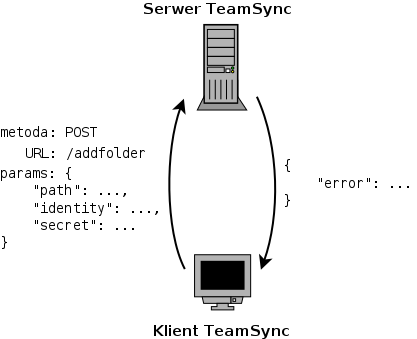
\includegraphics[width=230pt]{figures/metaddfolder.png}
  \end{center}
  \caption{Komunikacja w systemie \emph{TeamSync} podczas wywoływania metody \texttt{addfolder} --- tworzenie folderu.}
  \label{picmetgetfolders}
\end{figure}

Użytkownik ma możliwość wyboru pomiędzy rodzajem dodawanego katalogu --- inicjacja własnego lub dołączenie do już istniejącego, stworzonego przez innego użytkownika folderu. Podczas obydwóch tych operacji przeglądarkowy interfejs graficzny wysyła do serwera zapytanie metodą \texttt{POST} na adres \texttt{http://<adres oraz port serwera TeamSync>\-/addfolder}. W parametrach żądania znajdują się:

\begin{itemize}[noitemsep]
  \item \emph{path} --- bezwzględna ścieżka do folderu, którego zawartość od tej pory będzie synchronizowana z pozostałymi użytkownikami,
  
  \item \emph{identity} --- zadeklarowana przez użytkownika tożsamość, czyli nazwa użytkownika, jaka będzie wyświetlana innym węzłom,
  
  \item \emph{secret} --- za jego pomocą BitTorrent Sync odnajdzie w sieci pozostałych użytkowników; jeśli ten parametr pozostanie pusty, serwer stworzy nowy folder (nie w fizycznym sensie, lecz w logicznym --- doda podany w parametrze \emph{path} folder do folderów współdzielonych).
\end{itemize}

Serwer otrzymując żądanie z powyższymi parametrami, przekazuje je poprzez zapytanie \texttt{HTTP} do BitTorrent Sync API, za pomocą funkcji \texttt{add\_folder} (dokładny opis metody znajduje się w sekcji \ref{btsyncapiproto}). Jeśli podstawowa walidacja wprowadzanych danych się nie powiedzie, lub jeśli BitTorrent Sync API zwróci błąd, serwer oprócz zwrócenia odpowiedzi z treścią błędu nie wykona żadnych dodatkowych instrukcji.

W przypadku powodzenia serwer musi wykonać następujące czynności:

\begin{description}[noitemsep]
  \item[Utworzenie folderów \texttt{.Comments} oraz \texttt{.Users}] --- jeśli użytkownik nie dołącza do istniejącego folderu, tylko inicjuje swój katalog, musi stworzyć lokalizacje, do których pozostali użytkownicy będą mogli dopisywać pliki ze swoimi danymi (\texttt{.Users}) oraz komentarze (\texttt{.Comments}).
  
  \item[Uaktualnienie folderu \texttt{.Users}] --- aby inni użytkownicy mogli zobaczyć nowy węzeł w swoim folderze, użytkownik dołączający do katalogu musi umieścić w folderze \texttt{.Users} swoje dane --- identyfikator oraz tożsamość.
  
  \item[Uaktualnienie pliku konfiguracyjnego] --- do słownika \texttt{identities} --- przechowującego wszystkie tożsamości użytkownika --- w pliku konfiguracyjnym (\texttt{config.json}), dodawana jest nowa tożsamość.
\end{description}

Po wykonaniu powyższych czynności serwer zwraca komunikat do aplikacji klienckiej o powodzeniu operacji, a w przeglądarce odświeżana jest lista folderów.

\subsubsection*{Usuwanie folderu}

\begin{figure}[h!]
  \vspace{5pt}
  \begin{center}
    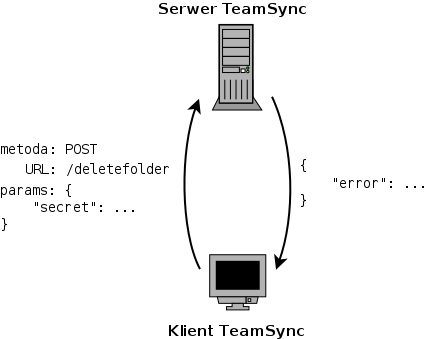
\includegraphics[width=240pt]{figures/metdeletefolder.png}
  \end{center}
  \caption{Komunikacja w systemie \emph{TeamSync} podczas wywoływania metody \texttt{addfolder} --- tworzenie folderu.}
  \label{picmetdeletefolder}
\end{figure}

Usuwanie katalogu odbywa się poprzez wysłanie do serwera żądania \texttt{HTTP} za pomocą metody \texttt{POST} na adres \texttt{http://<adres oraz port serwera TeamSync>\-/deletefolder}. Parametrem przesyłanym wewnątrz zapytania jest \emph{secret} folderu. Serwer nie robi nic poza przesłaniem \emph{secreta} za pomocą funkcji \texttt{remove\_folder} protokołu BitTorrent Sync API (dokładny opis funkcji \texttt{remove\_folder} w sekcji \ref{btsyncapiproto}) i  przekazuje odpowiedź --- o pomyślnym lub niepomyślnym usunięciu --- do klienta.

W przypadku niepowodzenia rola serwera kończy się na przekazaniu wyniku. Natomiast jeśli usunięcie folderu z listy synchronizowanych katalogów przebiegnie pomyślnie, serwer musi zmodyfikować plik konfiguracyjny \texttt{config.json} w celu usunięcia ze zmiennej \texttt{identities} tożsamości, której użytkownik już nie będzie potrzebował, ponieważ folder stanowiący jej środowisko przestał istnieć.

\subsection{Komentarze}

\label{comments}

Aplikacja TeamSync nie umożliwia usuwania komentarzy przez użytkowników nawet w przypadku gdy osobą, która chciałaby usunąć wypowiedź z systemu, jest jej autor. Usunięcie komentarza można zastąpić poprzez zmodyfikowanie lub całkowite usunięcie jego treści, natomiast obecność wypowiedzi w systemie będzie zawsze widoczna.

\subsubsection*{Czytanie komentarzy}

\begin{figure}[h!]
  \vspace{5pt}
  \begin{center}
    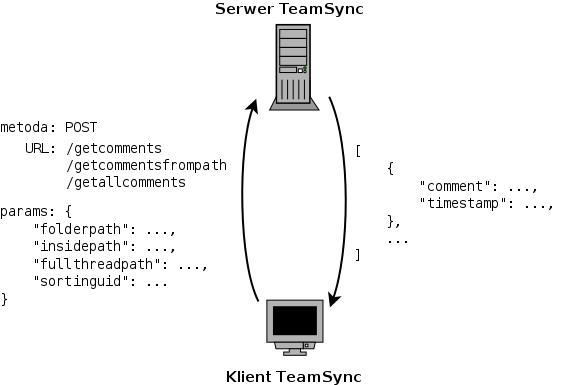
\includegraphics[width=320pt]{figures/metgetcomments.png}
  \end{center}
  \caption{Komunikacja w systemie \emph{TeamSync} podczas wywoływania metod \texttt{getcomments}, \texttt{getallcomments} oraz \texttt{getcommentsfrompath} --- czytanie komentarzy.}
  \label{picmetdeletefolder}
\end{figure}

Główną czynnością aplikacji TeamSync podczas wyświetlania komentarzy jest pobranie ich z serwera i przeniesienie odpowiedzi serwera do listy \texttt{comments}, która jest główną strukturą wyświetlaną w sekcji komentarzy. Zawiera ona komentarze w takiej strukturze, w jakiej są one przeczytane przez serwer z plików wewnątrz folderu z wątkiem.

Pobieranie listy komentarzy inicjowane jest z kodu \texttt{javascript} przeglądarki, a użyte do tego celu zapytania różnią się w zależności od widoku (aby zapoznać się dokładniej z widokami, należy przeczytać dodatek \ref{views}), w którym użytkownik aktualnie się znajduje:

\begin{description}[noitemsep]
  \item[W widoku nowego wątku] nie są pobierane żadne komentarze. W momencie wprowadzenia danych i zatwierdzenia nowego wątku system automatycznie przechodzi do widoku aktualnego wątku.
  
  \item[W widoku aktualnego wątku] odświeżanie listy komentarzy odbywa się za pomocą funkcji \texttt{re\-freshComments} wywoływanej np. podczas przechodzenia do nowego wątku albo wprowadzenia nowego komentarza. Jej zadaniem jest wysłanie na URL serwera \texttt{http://<adres oraz port serwera TeamSync>\-/getcomments} zapytania metodą \texttt{POST}, wewnątrz którego znajdują się następujące dane:
  \begin{itemize}[noitemsep]
    \item \emph{fullthreadpath} --- pełna ścieżka lokalizacji wątku, niezbędna do pobrania listy komentarzy,
    \item \emph{sortinguid} --- identyfikator użytkownika, według którego mają zostać posortowane komentarze. Jeśli wartość ta pozostanie pusta (domyślnie), serwer posortuje komentarze według ich znaczników czasowych pobranych w momencie umieszczenia ich w systemie TeamSync. W przeciwnym wypadku (\emph{sortinguid} wskazuje któregoś z użytkowników), wypowiedzi zostaną posortowane w takiej kolejności, w jakiej zostały odczytane przez wskazanego w argumencie \emph{sortinguid} użytkownika. Serwer wówczas --- zanim zwróci w odpowiedzi listę komentarzy --- posortuje dane według struktury \texttt{readby}, wewnątrz której umieszczone są znaczniki czasowe momentu odczytania wiadomości przez wskazanego użytkownika (sortowanie komentarzy według różnych spójności zostało szczegółowo opisane w sekcji \ref{consistencies}).
  \end{itemize}
  Jak zostało opisane na początku sekcji --- serwer odpowiada listą komentarzy odczytanych z plików i w zależności od zawartości argumentu \emph{sortinguid} sortuje wyjściowe dane przed ich wysłaniem do klienta.

  \item[W widoku bieżącej lokalizacji] do zmiennej \texttt{comments} zostaną przypisane komentarze z odpowiedzi serwera na zapytanie wysłane przez funkcję \texttt{getCommentsFromPath} uruchamianą w kodzie \texttt{javascript} przeglądarki klienta. Funkcja ta wysyła żądanie metodą \texttt{POST} na adres URL serwera \texttt{http://<adres oraz port serwera TeamSync>\-/getcommentsfrompath} z danymi w formacie JSON:
  \begin{itemize}[noitemsep]
    \item \emph{folderpath} --- bezwzględna ścieżka synchronizowanego folderu.
    \item \emph{insidepath} --- lokalizacja wewnątrz folderu, z której poziomu będą pobierane wszystkie komentarze. Nie będą brane pod uwagę komentarze w wątkach umieszczonych wewnątrz poziomów, wgłąb lokalizacji.
  \end{itemize}
  Konieczność wysłania dwóch ścieżek zamiast jednej podyktowana jest faktem, iż w przypadku pobierania komentarzy z jednego wątku zmienna \emph{fullthreadpath} zawarta jest --- obok innych informacji, np. nazwie, znaczniku czasowym powstania itd. --- w obiekcie wyświetlanym przez graficzny interfejs. Podczas pobierania komentarzy z jednego wątku wystarczy przekazać tą zmienną serwerowi. Natomiast w obecnym wypadku pobierania komentarzy z całej lokalizacji, nie ma jednego konkretnego wątku, z którego można by pozyskać tą informację, więc zostało przyjęte rozwiązanie, w którym klient wysyła dwie ścieżki, a serwer łączy je w całość (łącznie z katalogiem \texttt{.Comments} ścieżki łączone są na wzór \texttt{<folderpath>/.Comments/<insidepath>}) i dopiero z tak uzyskanej ścieżki pobierane są komentarze.
  
  \item[W widoku wszystkich komentarzy] w kodzie skryptu interfejsu uruchamiana jest nie przyjmująca żadnego argumentu funkcja \texttt{get\-All\-Comments}. Jej zadaniem jest wysłanie metodą \texttt{POST} na adres URL serwera \texttt{http://<adres oraz port serwera TeamSync>/getallcomments} bezwzględnej ścieżki synchronizowanego folderu. Serwer po jej odebraniu pobierze wszystkie komentarze napisane wewnątrz katalogu niezależnie od poziomu zagłębienia wewnątrz niego.
  
  \item[W widoku wszystkich komentarzy użytkownika] procedura uzyskiwania od serwera wyświetlanych postów wygląda identycznie jak w przypadku widoku wszystkich komentarzy. Jedyną różnicą w sposobie ich wyświetlania jest filtrowanie ich po stronie klienta według \emph{uid} autora wypowiedzi. Użytkownik wybierając autora, którego komentarze chciałby wyświetlić, w rzeczywistości pobiera wszystkie wypowiedzi z folderu i dopiero po ich uzyskaniu nakładany jest filtr. Dzięki takiemu podejściu możliwe jest szybsze oglądanie komentarzy różnych użytkowników, ponieważ pobierane one są raz. Zmieniając autora, zmieniane jest tylko filtrowanie wypowiedzi.
\end{description}

\subsubsection*{Pisanie komentarzy}

\begin{figure}[h!]
  \vspace{5pt}
  \begin{center}
    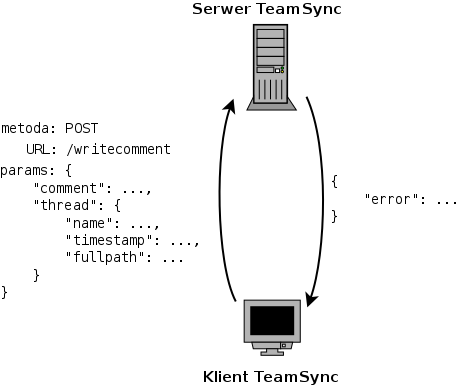
\includegraphics[width=250pt]{figures/metwritecomment.png}
  \end{center}
  \caption{Komunikacja w systemie \emph{TeamSync} podczas wywoływania metody \texttt{writecomment} --- pisanie komentarzy.}
  \label{picmetdeletefolder}
\end{figure}

Użytkownik przeglądając komentarze, może odpowiadać na nie tylko w przypadku, gdy przegląda je w widoku wątku (aby zapoznać się dokładniej z widokami, należy przeczytać dodatek \ref{views}). Nie ma możliwości odpisywania odpowiedzi na komentarz, nie znając kontekstu całego wątku, gdyż może to doprowadzić do nieporozumień między użytkownikami. Dlatego też możliwość komentowania we wszystkich widokach oprócz widoku wątku została zablokowana.

W widoku wątku --- na końcu konwersacji po obecnie ostatnim poście --- znajduje się pole tekstowe, gdzie użytkownik może wpisać treść swojej odpowiedzi, a następnie kliknąć przycisk, który metodą \texttt{POST} wysyła na adres \texttt{http://<adres oraz port serwera TeamSync>/\-writecomment} żądanie zawierające obiekt \texttt{JSON} z wartościami o następujących kluczach:

\begin{itemize}[noitemsep]
 \item \emph{comment} --- treść komentarza wpisana przez użytkownika,
 \item \emph{thread} --- obiekt JSON zawierający dane dotyczące aktywnego wątku (tego, w którym odpowiada użytkownik), które zawiera nastepujące informacje:
 \begin{itemize}[noitemsep]
  \item \emph{aaa} --- dsadsadasda
  \item \emph{dsadasdsa} --- dasczxczxcxz
 \end{itemize}
\end{itemize}

\begin{figure}[htb!]
\label{newcommentrequest}
  \begin{verbatim}
{
    "comment": "Treść nowego komentarza", 
    "thread": {
        "numberofcomments": 7, 
        "name": "Testowy tytul", 
        "timestamp": "1438513896000", 
        "lastcomment": "1439395572000", 
        "path": "/", 
        "fullpath": "/home/user/aaa/.Comments/1438513896000@#&$Testowy tytul", 
        "type": "thread", 
        "unreadcomment": false
    }
}
  \end{verbatim}
  \caption{Przykładowe żądanie wysyłane do serwera podczas odpowiedzi na wątek.}
\end{figure}

Po otrzymaniu od klienta żądania z tymi danymi serwer za pomocą ścieżki \texttt{fullpath} wewnątrz słownika \texttt{thread} pobierze z serwera NTP znacznik czasowy (aby uwiarygodnić przykład, założono, że pobrany znacznik czasowy to \texttt{1439396297000}) i umieści w podanej lokalizacji (\texttt{/home/\-user/\-aaa/\-.Comments/\-1438513896000\@\#\&\$Testowy tytul}) nowy plik z komentarzem o nazwie \texttt{1439396\-297000\@\#\&\$2HI7KRUNS\-SONIUJKM\-RWXGOTIZ\-SHBGFIH}:

\begin{figure}[htb]
\begin{verbatim}
           {
               "comment": "Treść nowego komentarza",
               "timestamp": "1439396297000",
               "history": [
                   {
                       "comment": "Treść nowego komentarza",
                       "timestamp": "1439396297000"
                   }
               ], 
               "uid": "2HI7KRUNSSONIUJKMRWXGOTIZSHBGFIH",
               "readby": {
                   "2HI7KRUNSSONIUJKMRWXGOTIZSHBGFIH": "1439395604000"
               }
           }
\end{verbatim}
  \caption{Plik komentarza zapisany w wyniku otrzymania przez serwer  wyżej zaprezentowanego żądania.}
\end{figure}

\subsubsection*{Edycja komentarzy}

\begin{figure}[h!]
  \vspace{5pt}
  \begin{center}
    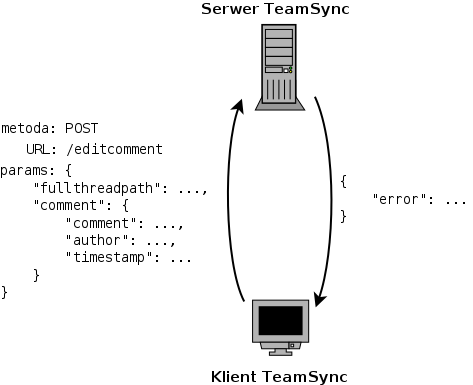
\includegraphics[width=260pt]{figures/meteditcomment.png}
  \end{center}
  \caption{Komunikacja w systemie \emph{TeamSync} podczas wywoływania metody \texttt{editcomment} --- edycja komentarzy.}
  \label{picmetdeletefolder}
\end{figure}

Modyfikacja komentarza może być dokonana tylko przez jego autora. Dzięki zastosowaniu takiego podejścia obniżone zostało ryzyko wystąpienia konfliktu podczas synchronizacji, ponieważ liczba osób mogących edytować plik komentarza została zredukowana do jednej.

Po zatwierdzeniu zmian do serwera wysyłane są dane niezbędne do odnalezienia komentarza w systemie plików i dopisania następnego wpisu do słownika \texttt{history} znajdującego się wewnątrz pliku z wypowiedzią wypowiedzi. Informacje wysyłane są za pomocą metody \texttt{POST} na adres \texttt{http://<adres oraz port\- serwera TeamSync>/\-editcomment}. Tymi danymi są:

\begin{itemize}[noitemsep]
  \item lokalizacja wątku --- pełna ścieżka folderu przechowującego pliki komentarzy oraz plik z metadanymi w dyskusji (plik \texttt{meta}),
  
  \item cały obiekt JSON zawierający dane komentarza w formie, w jakiej jest on odczytywany z pliku, z tą różnicą, że w zmiennej \texttt{comment} (zawierającej treść komentarza) znajduje się nowa, zmodyfikowana przez użytkownika wypowiedź.
\end{itemize}

Po otrzymaniu żądania zawierającego powyższe informacje serwer odtwarza tytuł pliku komentarza, posługując się zmiennymi \texttt{timestamp} oraz \texttt{uid}, otrzymując pełną ścieżkę komentarza. Wczytuje plik komentarza zapisany na dysku, modyfikuje zmienną \texttt{comment} treścią podaną przez użytkownika i dodaje do słownika \texttt{history} nowy element zawierający pobrany znacznik czasowy z serwera \emph{NTP} oraz nową treść wypowiedzi. Następnie zapisuje komentarz w tym samym pliku.

Aby zaoszczędzić czas, który tracony jest na odczytywanie pliku z systemu plików, serwer mógłby pominąć ten etap i --- po dodaniu wpisu do zmiennej \texttt{history} --- od razu komentarz zapisać. Jednak dane przesyłane z przeglądarki do serwera zawierają informacje nadmiarowe dotyczące interfejsu graficznego, które są zbędne dla serwera. Do poprawnego działania funkcji serwerowi wystarczyłyby dane:

\begin{itemize}[noitemsep]
  \item \emph{comment} --- nowa treść komentarza,
  
  \item \emph{timestamp} --- znacznik czasowy utworzenia komentarza (potrzebne do identyfikacji pliku w folderze wątku),
  
  \item \emph{uid} --- autor komentarza (potrzebne do identyfikacji pliku w folderze wątku),
  
  \item \emph{fullthreadpath} --- pełna ścieżka wątku, w którym komentarz jest fizycznie zapisany.
\end{itemize}

Jednakże zdecydowano się na przesłanie całej struktury komentarza ze względu na niewielką nadmiarowość danych oraz większe możliwości manipulacji zapisywaniem komentarza podczas ewentualnych ulepszeń aplikacji TeamSync w przyszłości.

\subsection{Wątki}

Użytkownicy mają możliwość tworzyć komentarze oraz je edytować, natomiast \emph{TeamSync} nie umożliwia usuwania ich ze względu na zachowanie spójności logicznej dyskusji. W przypadku wątków możliwości użytkowników zostały dodatkowo ograniczone --- edytowanie wątku zostało zminimalizowane wyłącznie do edycji treści pierwszego komentarza. Ze względu na fakt, iż była ona omówiona wcześniej (sekcja \ref{comments}), omówiona zostanie wyłącznie procedura dodawania do systemu nowej dyskusji.

\subsubsection*{Tworzenie nowego wątku}

\begin{figure}[h!]
  \vspace{5pt}
  \begin{center}
    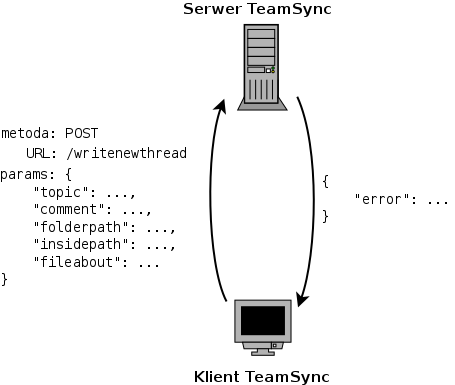
\includegraphics[width=250pt]{figures/metwritenewthread.png}
  \end{center}
  \caption{Komunikacja w systemie \emph{TeamSync} podczas wywoływania metody \texttt{writenewthread} --- tworzenie nowego watku.}
  \label{picmetdeletefolder}
\end{figure}

Użytkownik tworząc nowy wątek, wysyła --- poprzez aplikację kliencką w przeglądarce --- do serwera żądanie \texttt{HTTP} za pomocą metody \texttt{POST} na adres \texttt{http://<adres oraz port\- serwera TeamSync>/\-writenewthread}. W zapytaniu przesyłane sa następujące parametry:

\begin{itemize}[noitemsep]
  \item \emph{topic} --- tytuł wątku wprowadzony przez użytkownika,
  
  \item \emph{comment} --- treść pierwszego komentarza wprowadzona przez użytkownika,
  
  \item \emph{folderpath} --- bezwzględna ścieżka synchronizowanego folderu w lokalnym systemie operacyjnym użytkownika,
  
  \item \emph{insidepath} --- lokalizacja wątku wewnątrz folderu nie uwzględniając samego katalogu przechowującego wątek,
  
  \item \emph{fileabout} --- nazwa pliku wybranego przez użytkownika, którego dotyczyć będzie wątek.
\end{itemize}

Po otrzymaniu żądania serwer w pierwszej kolejności pobiera znacznik czasowy z serwera NTP, który jest potrzebny do wygenerowania nazwy folderu z nowym wątkiem łączącej ze sobą pobrany znacznik, identyfikator użytkownika oraz separator nazwy (dokładny opis separatora znajduje się w sekcji \ref{filenames}). Przyjmując jako separator użyty w implementacji ciąg znaków: \texttt{@\#\&\$}, nazwa katalogu wygląda następująco:

\begin{verbatim}
               < znacznik czasowy >@#&$< identyfikator użytkownika >
\end{verbatim}

Następnie serwer ustala pełną ścieżkę wątku z przekazanych w żądaniu parametrów \texttt{folderpath} oraz \texttt{insidepath}:

\begin{verbatim}
            folderpath/.Comments/insidepath/< nazwa katalogu z wątkiem >
\end{verbatim}

Po ustaleniu pełnej lokalizacji wątku serwer tworzy folder o podanej wyżej ścieżce i umieszcza w nim plik \texttt{meta} uzupełniając go wartościami podanymi przez użytkownika w żądaniu. Poniżej przedstawiono przykładowe parametry przesyłane w celu stworzenia nowego wątku w postaci obiektu \texttt{JSON}.

\begin{figure}[htb]
\begin{verbatim}
                {
                    "topic": "Testowy tytuł", 
                    "comment": "Przykładowa treść komentarza", 
                    "insidepath": "/abc", 
                    "fileabout": "aaa", 
                    "folderpath": "/home/user/testowy katalog"
                }
\end{verbatim}
  \caption{Parametry przesyłane w przykładowym zapytaniu tworzącym nowy wątek.}
\end{figure}

Według parametrów zawartych w przykładzie nowy wątek będzie miał tytuł \texttt{Testowy tytuł}, a treść pierwszego komentarza to \texttt{Przykładowa treść komentarza}. Lokalizacja uwspólnionego folderu, wewnątrz którego zamieszczany jest wątek, to \texttt{/home/user/\-testowy katalog}, natomiast wątek umieszczony jest jeden poziom głębiej, w katalogu \texttt{abc}. Dodatkowo utworzona dyskusja dotyczy pliku o pełnej ścieżce \texttt{/home/user/\-testowy katalog/\-abc/aaa}.

W wyniku otrzymania powyższego żądania --- zakładając, że pobrany znacznik czasowy to \texttt{1441566\-810000}, a identyfikator użytkownika zakładającego wątek to \texttt{FWZPQQKU\-E3JPQKWY5\-57FERJ4S\-D3BSFMM} --- serwer utworzy wątek w lokalizacji o pełnej ścieżce:

\begin{verbatim}
       /home/user/testowy katalog/.Comments/abc/
                         1441566810000@#&$FWZPQQKUE3JPQKWY557FERJ4SD3BSFMM
\end{verbatim}

Wewnątrz tego folderu zostanie umieszczony plik \texttt{meta} oraz plik pierwszego komentarza o podanych poniżej zawartościach.

\begin{figure}[htb]
\begin{verbatim}
                {
                    "topic": "Testowy tytuł", 
                    "timestamp": "1441566810000", 
                    "fileabout": "/abc/aaa", 
                    "uid": "FWZPQQKUE3JPQKWY557FERJ4SD3BSFMM"
                }
\end{verbatim}
  \caption{Zawartość pliku \texttt{meta} utworzonego w wyniku otrzymania przykładowego żądania.}
\end{figure}

\begin{figure}[htb]
\begin{verbatim}
           {
               "comment": "Przykładowa treść komentarza", 
               "timestamp": "1441566810000", 
               "history": [
                   {
                       "comment": "Przykładowa treść komentarza", 
                       "timestamp": "1441566810000"
                   }
               ], 
               "readby": {
                   "FWZPQQKUE3JPQKWY557FERJ4SD3BSFMM": "1441566810000"
               }, 
               "uid": "FWZPQQKUE3JPQKWY557FERJ4SD3BSFMM"
           }
\end{verbatim}
  \caption{Zawartość pliku z pierwszym komentarzem utworzonego w wyniku otrzymania przykładowego żądania.}
\end{figure}

W pliku \texttt{meta} zapisanym w folderze w wyniku otrzymania przez serwer przykładowego żądania umieszczony został tytuł \texttt{Testowy tytuł} wpisany przez użytkownika, znacznik czasowy zwrócony przez serwer NTP, identyfikator autora wątku oraz wewnętrzna ścieżka do pliku, na którego temat powstała dyskusja. Jeśli wątek nie dotyczyłby żadnego z plików, wartość \texttt{fileabout} byłaby równa \texttt{<brak>}.

Zapisywanie plików komentarzy zostało dokładniej opisane w sekcji \ref{comments}.

\section{Aplikacja przeglądarkowa}

Wśród podstawowych założeń implementacyjnych aplikacji \emph{TeamSync} --- poza założeniami wynikającymi z zastosowania systemu \emph{BitTorrent Sync} jako narzędzia odpowiedzialnego za wymianę danych --- znajdują się wymagania dotyczące interakcji człowieka z systemem. Podstawowymi założeniami --- oprócz prostoty interfejsu oraz łatwości jego obsługi --- w tym zakresie są: częstość odświeżania informacji oraz szybkość działania.

Aby sprostać powyższym wymaganiom i zachować interfejs w statycznym środowisku --- jakim jest serwer WWW --- zastosowano w pracy asynchroniczne zapytania (\emph{AJAX} \cite{ajax}) między częścią serwerową i kliencką. Podczas niemal każdej z czynności wykonywanych przez użytkownika w interfejsie odświeżana jest większa część danych pokazywanych użytkownikowi:

\begin{itemize}[noitemsep]
  \item komentarze,
  \item listy wątków,
  \item listy plików/katalogów przechowywanych w synchronizowanym folderze.
\end{itemize}

\subsubsection*{Two-way data binding}

Ważnym mechanizmem umożliwiającym dynamiczną zmianę treści strony unikając jej całkowitego przeładowania, jest tzw. ,,\emph{two-way data binding}'' zaimplementowany przez twórców narzędzia \emph{AngularJS}. Interfejs działający w tym systemie wyświetla elementy \emph{modelu}, które użytkownik zaimplementuje --- w przypadku aplikacji \emph{TeamSync} wewnątrz modelu znajdują się np. wszystkie listy przechowujące dane (listy plików, wątków, komentarzy, identyfikator użytkownika, itp.) albo ustawienia aplikacji.

Ogólna koncepcja metody ''\emph{two-way data binding}'' polega na zrealizowaniu jednocześnie dwóch następujących założeń dotyczących sposobu prezentacji w interfejsie danych pochodzących z modelu:

\begin{enumerate}[noitemsep]
  \item Jeśli dane zmienią się wewnątrz modelu, zmiana nastąpi również w interfejsie graficznym.
  
  \item Jeśli dane prezentowane w interfejsie graficznym zostaną zmienione, zmiana nastąpi również w \emph{modelu}.
\end{enumerate}

W ten sposób --- korzystając z pierwszego założenia --- jeśli wewnątrz kodu przeglądarki nastąpi odświeżenie dowolnej zmiennej (np. listy plików) poprzez zapytanie asynchroniczne, zostanie ona z natychmiastowym skutkiem zmieniona w interfejsie graficznym. Przykładem wykorzystania drugiego założenia może być sytuacja, w której użytkownik chce posortować wątki według żądanego kryterium. Wprowadzając odmienne kryterium niż obecne, wywołuje szereg operacji nie na zmiennych wyświetlanych w interfejsie, lecz na zmiennych wewnątrz modelu.

Dokładniejszy opis i przykłady obydwóch powyższych założeń zostaną przedstawione w następnych podrozdziałach.

\subsection{Wyświetlanie plików}

Podczas odświeżania listy plików, w kodzie \emph{javascript} interfejsu wysyłane jest asynchroniczne zapytanie metodą \texttt{POST}, a cała struktura, którą przeglądarka otrzyma w odpowiedzi od serwera, umieszczana jest wewnątrz zmiennej \texttt{files} reprezentującej listę plików. Aby przedstawić całą otrzymaną listę w interfejsie użytkownika, należy umieścić ją w strukturze, która umożliwi czytelne odwzorowanie listy. W tym celu posłużono się znacznikami \texttt{ul} oraz \texttt{li}, które są stworzone z myślą o prezentacji list (ul = unordered list). Przykładowe użycie znaczników \texttt{ul} oraz \texttt{li} wygląda następująco:

\begin{figure}[htb]
\begin{verbatim}
                            <ul>
                                <li>Element 1</li>
                                <li>Element 2</li>
                                <li>Element 3</li>
                            </ul>
\end{verbatim}
\end{figure}

\emph{AngularJS} umożliwia dynamiczną manipulację elementami listy poprzez dyrektywę \texttt{ng-repeat} dodawaną do tego znacznika, który ma zostać powtórzony. W przypadku powyższego przykładowego kodu dyrektywa \texttt{ng-repeat} zostanie dodana do pierwszego znacznika \texttt{li}. Jeśli w modelu istniałaby zmienna \texttt{list}, będąca tablicą zawierającą trzy elementy o typie znakowym: ,,\texttt{Element 1}'', ,,\texttt{Element 2}'' oraz ,,\texttt{Element 3}'', poniższy kod w pliku \emph{HTML} byłby jednakowy z wcześniejszym:

\begin{figure}[htb]
\begin{verbatim}
                 <ul>
                     <li ng-repeat="item in list">{{ item }}</li>
                 </ul>
\end{verbatim}
\end{figure}

Dyrektywa \texttt{ng-repeat} tworzy pętlę przechodzącą po wszystkich elementach listy, która wewnątrz każdego znacznika \texttt{li} umieszcza element, którego aktualnie dotyczy iteracja. Podwójny nawias ,,\{'' służy do umieszczania zawartości przechowywanych wewnątrz zmiennych, które służą jako iterator (w powyższym przypadku iteratorem jest zmienna \texttt{item}).Jeśli modyfikacji (na przykład podczas asynchronicznego zapytania do serwera i zaktualizowania listy) ulegnie lista \texttt{list}, wewnątrz której odbywa się iteracja w dyrektywie \texttt{ng-repeat}, zmiana zostanie przeniesiona na interfejs. Spełnione zostanie pierwsze założenie metody \emph{two-way data binding} --- zmiana modelu wpłynie na interfejs graficzny.

Dyrektywa \texttt{ng-repeat} została wykorzystana w aplikacji \emph{TeamSync} np. do prezentowania listy plików. Zmienna \texttt{files}, w której umieszczane są elementy pochodzące z odpowiedzi serwera, stanowi listę, wewnątrz której dyrektywa \texttt{ng-repeat} iteruje, wyświetlając odpowiednie informacje użytkownikowi.

\begin{figure}[htb]
\begin{verbatim}
           <ul>
               <li ng-repeat="file in files">{{ file.name }}</li>
           </ul>
\end{verbatim}
\end{figure}

Ze względu na założenia metody \emph{two-way data binding}, w momencie odebrania odpowiedzi od serwera, przeglądarka natychmiast wyświetli aktualną listę plików, czego efektem jest niezbędna dynamika aplikacji. Ponieważ zawarte wewnątrz listy \texttt{files} elementy są obiektami \texttt{JSON}, wewnątrz podwójnych nawiasów klamrowych musiała zostać umieszczona któraś z wartości obiektu, a nie cały obiekt. Skoro użytkownik musi widzieć nazwę pliku, aby móc nawigować po synchronizowanym folderze, została użyta wartość obiektu \texttt{file}, której kluczem jest \texttt{name} (nazwa).

W podobny sposób działają wszystkie dynamiczne elementy strony interfejsu graficznego, które są modyfikowane zarówno przez serwer, jak i użytkownika. Przykładem zmiennych, które prezentowane sa w podobny sposób do plików, są:

\begin{itemize}[noitemsep]
  \item lista folderów,
  \item lista wszystkich użytkowników w folderze,
  \item lista komentarzy,
  \item lista wątków.
\end{itemize}


\subsection{Filtrowanie komentarzy}

Wyszukiwanie wewnątrz komentarzy wpisywanych przez użytkownika fraz w aplikacji \emph{TeamSync} odbywa się w całości po stronie klienta, dzięki czemu jest bardzo szybkie i dynamiczne. Filtr jest uaktualniany i zaczyna działać podczas wprowadzenia każdego znaku. Odbywa się to dzięki użyciu słowa kluczowego \texttt{filter} dostępnego w systemie \emph{AngularJS}, którego umieszczenie w odpowiedni sposób wewnątrz kodu HTML aplikacji spowoduje wykluczenie ze zbioru danych elementów niepasujących do wzorca.

Użycie funkcji \texttt{filter} zostanie opisane na kodzie HTML z wcześniejszego przykładu, do którego dodano funkcjonalność filtrowania:

\begin{figure}[htb]
\begin{verbatim}
      <ul>
          <li ng-repeat="item in list | filter:testFilter">{{ item }}</li>
      </ul>
\end{verbatim}
\end{figure}

Znak ,,\texttt{|}'' jest znakiem, który powoduje poddanie zbioru danych sprzed tego znaku (w tym przykładzie jest to lista \texttt{list}) działaniu operacji po tym znaku --- filtrowaniu, lub sortowaniu (w tym przykładzie jest to filtrowanie). Słowo \texttt{filter} jest słowem kluczowym oznaczającym wykonywanie filtrowania na zbiorze danych \texttt{list}. \texttt{testFilter} jest zmienną pochodzącą z modelu, wewnątrz której przechowywana jest wartość filtru. Jeśli byłby spełnione poniższe warunki:

\begin{figure}[htb]
\begin{verbatim}
               testFilter = "1"
               list = ["Element 1", "Element 2", "Element 3"]
\end{verbatim}
\end{figure}

Wewnątrz znacznika \texttt{ul} zostałyby wyświetlone wyłącznie te elementy \texttt{li}, których zawartość zawierałaby znak ,,$1$''. Posługując się obecnym przykładem, użytkownik wyświetlając powyższy kod z powyższymi danymi wewnątrz modelu zobaczyłby w swojej przeglądarce wyłącznie pierwszy element o treści \texttt{Element 1}.

Wewnątrz aplikacji \emph{TeamSync} funkcjonalność słowa kluczowego \texttt{filter} została wykorzystana do filtrowania tresci komentarzy w poszukiwaniu żądanego przez użytkownika słowa. Wszystkie komentarze aktualnie wyświetlane na ekranie zostają poddawane filtracji w poszukiwaniu wprowadzonej frazy. W uproszczonej wersji kod HTML tej funkcjonalności w aplikacji \emph{TeamSync} wygląda w następujący sposób:

\begin{figure}[htb]
\begin{verbatim}
         <ul>
             <li ng-repeat="comment in comments | filter: searchphrase">
         </ul>
\end{verbatim}
\end{figure}

Zmienna \texttt{comments} jest listą, do której asynchronicznie pobierane są z serwera komentarze w formie obiektów \texttt{JSON}. Podobnie jak w wyświetlaniu plików, również tutaj podczas aktualizacji tej zmiennej w modelu (dzięki technice \emph{two-way data binding}) natychmiast aktualizowane są elementy w interfejsie graficznym. Po słowie kluczowym \texttt{filter} --- sygnalizującym działanie filtra zbioru danych \texttt{comments} --- znajduje się zmienna \texttt{searchphrase}, której wartość jest ciągiem znaków wyszukiwanym wśród komentarzy. Wyświetlany zbiór wypowiedzi (spośród listy \texttt{comments}) zostanie ograniczony tylko do tych, które zawierają frazę wpisaną do zmiennej \texttt{searchphrase}.

Podczas tej operacji system \emph{AngularJS} skorzysta z drugiego założenia metody \emph{two-way data binding} --- użytkownik wprowadzając w interfejsie graficznym szukaną frazę, automatycznie uaktualni zmienną \texttt{searchphrase} w modelu. Z kolei zmienna \texttt{searchphrase} pobrana z modelu zostanie użyta do wyświetlenia zubożonego zbioru komentarzy o te, które nie pasują do wpisanego wzorca.

W systemie \emph{AngularJS} możliwe jest stosowanie wielu filtrów na tym samym zbiorze danych. W aplikacji \emph{TeamSync} zostało to wykorzystane, aby dodatkowo móc wyfiltrować te wiadomości, które zostały umieszczone przez konkretnych użytkowników.

\chapter{Zakończenie}

W ramach niniejszej pracy zaprojektowano oraz zaimplementowano system służący do wymiany zarówno plików, jak i komentarzy. System \emph{TeamSync} w części transportu danych opiera się na aplikacji \emph{BitTorrent Sync} działającej na protokole BitTorrent. Komunikację pomiędzy systemami umożliwia API stworzone przez producentów aplikacji \emph{BitTorrent Sync}, które umożliwia kontrolowanie synchronizowanych danych. Wewnątrz stworzonego systemu \emph{TeamSync} zostało zaimplementowanych wiele funkcjonalności zarówno podstawowych (wymiana komentarzy), jak i dodatkowych (wyszukiwanie, filtrowanie). Wszystkie najistotniejsze funkcje systemu \emph{TeamSync} zostały wymienione poniżej.

Użytkownicy mogą zarządzać (dodawać, modyfikować oraz usuwać) folderami, które współdzielą z innymi użytkownikami w sieci. System \emph{TeamSync} zapewnia pełną nawigację po synchronizowanych katalogach z poziomu interfejsu użytkownika. Interfejs dodatkowo umożliwia tworzenie przez użytkowników nowych wątków, wypowiadanie się wewnątrz nich oraz edycję komentarzy wraz z możliwością przeglądania historii zmian. Tworzone wątki mogą (lecz nie muszą) dotyczyć dowolnych plików zawartych w folderze.

Poza operacjami dokonywanymi na komentarzach system umożliwia swobodne wyszukiwanie informacji, poprzez narzędzia sortujące i filtrujące wypowiedzi oraz wątki. Dyskusje mogą zostać posortowane alfabetycznie, chronologicznie, według największej ilości postów oraz według najpóźniej dodanej odpowiedzi. Użytkownik ma możliwość filtrować wątki według procentowego udziału wybranych użytkowników w dyskusji. System również umożliwia wyszukiwanie wpisywanych przez użytkownika fraz w komentarzach z możliwością zmiany zbioru komentarzy --- wątek, wszystkie komentarze, wszystkie komentarze konkretnego użytkownika. Dostępny jest też tryb statystyk, w którym wyświetlana jest ilość wypowiedzi każdego z użytkowników oraz ich procentowy udział w zbiorze komentarzy.

Szczegółowy model systemu, jego architektura, ogólny sposób działania, konfiguracja oraz impementacja zostały opisane w poprzednich rozdziałach niniejszej pracy. 

System \emph{TeamSync} został zaimplementowany w sposób umożliwiający jego dalszy rozwój. Wśród dodatkowych funkcjonalności, które mogłyby zostać zaimplementowane bez konieczności dokonywania dużych zmian w strukturze kodu (zarówno części klienckiej, jak i serwerowej) są:

\begin{enumerate}[noitemsep]
  \item Wykrywanie typów plików obrazów lub muzycznych (np. \texttt{jpg}, \texttt{mp3}) i możliwość ich podglądu (lub odtworzenia w przypadku plików muzycznych).
  
  \item Dostosowanie aplikacji TeamSync do pracy z systemami operacyjnymi: Windows oraz MacOS.
  
  \item Możliwość dokonywania zmian w synchronizowanym folderze (np. wyłączenie tzw. ,,trackera'', wyszukiwanie innych użytkowników za pomocą DHT \cite{dht}.
  
  \item Dodanie kilku dodatkowych ustawień dotyczących graficznego interfejsu:
  \begin{itemize}[noitemsep]
    \item możliwość zmiany formatu daty wyświetlanej obok komentarzy,
    \item możliwość definiowania własnego koloru czcionki lub ramki, wewnątrz której wyświetlane są komentarze użytkownika,
    \item możliwość wybrania przez użytkownika pliku graficznego (tzw. ,,avatara'') umieszczanego obok jego nazwy na liście użytkowników oraz obok każdego komentarza.
  \end{itemize}
\end{enumerate}

% All appendices and extra material, if you have any.
\cleardoublepage\appendix%
\chapter{Instrukcja użytkownika}

\section{Graficzny interfejs użytkownika}

\label{gui}

Posługiwanie się przez użytkownika wszystkimi wymienionymi funkcjonalnościami powinno być łatwe oraz intuicyjne. Dostępne opcje zostały zaimplementowane w taki sposób, aby przeciętny odbiorca oprogramowania mógł dokonać żądanych działań w jak najkrótszym czasie i z jak najmniejszym wysiłkiem. Dostęp do większości funkcji uzyskiwany jest poprzez kliknięcia myszką komputera, która jest łatwiejszym sposobem nawigowania przez użytkowników wewnątrz aplikacji niż klawiatura.

Interakcja odbiorcy z aplikacją TeamSync poprzez klawiaturę została zredukowana do niezbędnego minimum, czyli wprowadzania danych (komentarzy, tytułów wątków, tożsamości oraz łańcucha \emph{secret} podczas dodawania nowego folderu itp.) oraz wyszukiwania fraz tekstowych. Nie ma możliwości, aby użytkownik nawigując wewnątrz systemu musiał ręcznie wpisywać np. nazwę innego użytkownika będącego w systemie, którego komentarze chciałby wyświetlić --- zamiast wprowadzania tych danych ręcznie, system wylistuje użytkowników pozostawiając tylko konieczność wyboru poprzez manipulację myszką.

\subsection*{Struktura graficzna aplikacji}

\begin{figure}[htb]
  \vspace{5pt}
  \begin{center}
    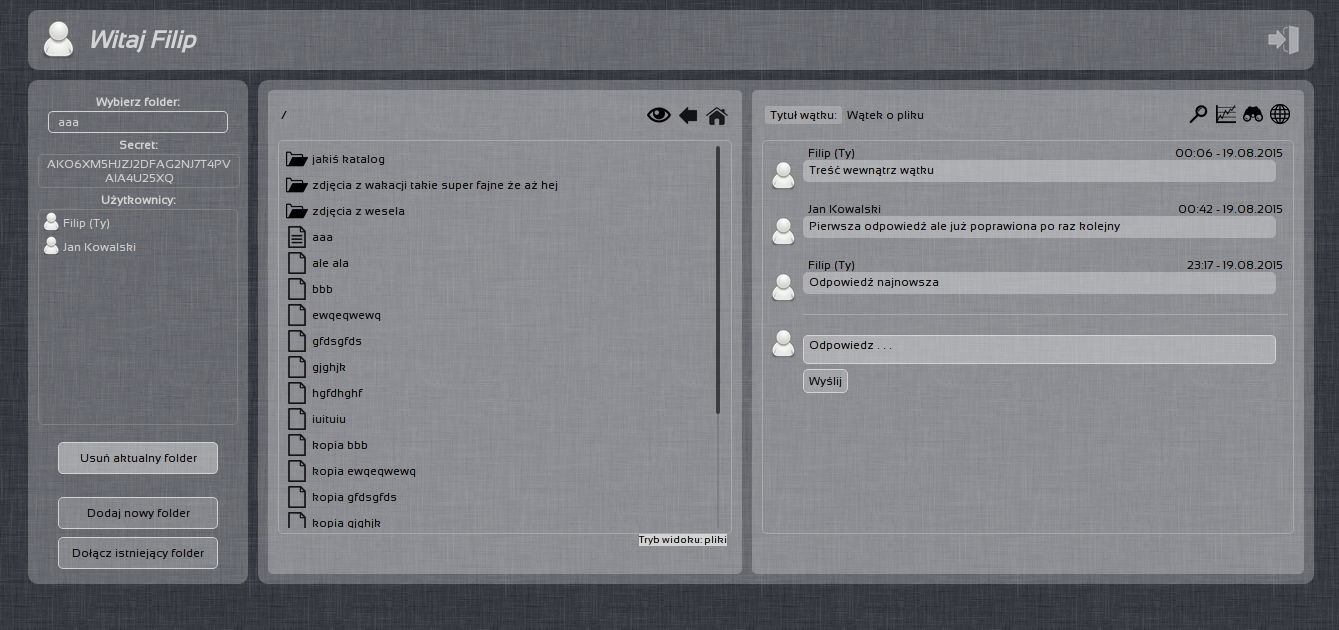
\includegraphics[width=400pt]{figures/filescomments.png}
  \end{center}
  \caption{Wygląd przykładowego folderu w graficznym interfejsie użytkownika.}
\end{figure}

Aby użytkownik łatwo odnalazł potrzebne mu funkcje ekran podzielony został na trzy części (nie licząc paska nagłówkowego) w układzie kolumnowym. Pierwsza --- część folderów --- służy do manipulacji synchronizowanymi katalogami. Druga --- środkowa --- służy do nawigacji po folderach oraz do przeglądania wątków, lecz nie wyświetlając wśród nich komentarzy. Trzecia natomiast przeznaczona jest do wyświetlania treści komentarzy i manipulowania zbiorem wyświetlanych wypowiedzi. Jeśli w danym momencie nie jest wybrany żaden z folderów z listy, dwie ostatnie części zajmujące główną część ekranu są nieaktywne.

W dalszej części podrozdziału omówione zostaną dokładniej przedstawione sekcje.

\subsubsection*{Sekcja folderów}

Jak opisano wcześniej, wewnątrz najmniejszej z trzech sekcji użytkownik może wykonywać operacje związane folderami, które współdzieli z innymi użytkownikami. Znajduje się w niej między innymi lista wszystkich zsynchronizowanych folderów (według ograniczeń systemu BitTorrent Sync może ich być maksymalnie $10$) wewnątrz kontrolki typu \emph{drop-down list} \cite{dropdownlist}, dzięki której użytkownik może w łatwy sposób dokonać wyboru.

Poniżej listy folderów znajdują się obszary, które po wybraniu katalogu wypełniają się odpowiednio danymi: ciągiem znaków tzw. \emph{secretem} oraz listą użytkowników, którzy przynależą do wybranego folderu. Aby ułatwić użytkownikowi identyfikację samego siebie spośród innych, do wyświetlanej nazwy jest dodawany ciąg znaków ,,(Ty)''.

Poza powyżej wymienionymi danymi w sekcji folderów znajdują się również przyciski umożliwiające usunięcie aktualnie wybranego folderu (przycisk jest nieaktywny, jeśli żaden folder nie został jeszcze wybrany) oraz dodanie nowego katalogu, które może odbyć się na dwa sposoby. Pierwszy zakłada, że folder jest inicjowany od zera i nie ma potrzeby wpisywania łańcucha \emph{secret}, ponieważ zostanie on wygenerowany przez system. Drugi wymaga jego podania i łączy wskazany z systemu plików pusty katalog z folderem innego użytkownika, od którego otrzymano łańcuch \emph{secret}. W obydwóch przypadkach konieczne jest podanie ścieżki do folderu, który ma być uwspólniony oraz tożsamości, czyli nazwy wyświetlanej dla innych użytkowników, mającej swój zasięg tylko wewnątrz katalogu.

\subsubsection*{Sekcja wątków}

Sekcja wątków składa się z nagłówka oraz części głównej zajmującej przeważający obszar całej sekcji. W nagłówku wyświetlana jest ścieżka aktualnej lokalizacji (nie bezpośrednia, lecz ta wewnątrz folderu, który będzie ,,korzeniem'' ścieżki), w której znajduje się użytkownik, zmieniająca się dynamicznie w interfejsie w miarę postępu nawigacji po katalogu.

Wewnątrz nagłówka, po przeciwnej stronie ścieżki znajdują się ikony funkcji, które pomagają w nawigacji oraz zmianie trybu widoku w głównej części sekcji. Naciśnięcie ikony prezentującej strzałkę skierowaną w lewo (,,do tyłu'') powoduje cofnięcie się ścieżki lokalizacji o jeden poziom. Uruchomienie funkcji ukrytej pod ikoną domu sprawia, że --- niezależnie od obecnej lokalizacji, w której się znajduje --- użytkownik zostanie sprowadzony do podstawowego poziomu w folderze --- jego ,,korzenia''.

Główna część sekcji służy do prezentacji plików oraz wątków w dwóch możliwych trybach, pomiędzy którymi przełączanie odbywa się za pomocą wciśnięcia kursorem myszki ikony zawierającej grafikę przedstawiającą oko, w nagłówku sekcji wątków.

\begin{description}[noitemsep]
  \item[Tryb plików] --- uruchamiając ten tryb, użytkownik może przeglądać zawartość synchronizowanego folderu w takiej postaci, w jakiej jest on zapisany na dysku. Uruchamiając kliknięciem myszy element z ikoną przedstawiającą folder użytkownik przechodzi do lokalizacji wewnątrz niego. Oprócz plików i katalogów wylistowanych w trybie plików, użytkownik widzi również wątki --- nie tylko te umieszczone w odpowiedniej lokalizacji ale też te przyporządkowane do konkretnych plików (jeśli do pliku jest przypisany wątek, ikona reprezentująca ten plik jest dostrzegalnie zmieniona, a po jej kliknięciu rozwijana jest lista wszystkich dyskusji dotyczących tego pliku).
  
  \item[Tryb wątków] --- przełączenie do tego trybu skutkuje wylistowaniem tylko i wyłącznie wątków napisanych wewnątrz folderu (niezależnie od lokalizacji), a uruchamianie funkcji nawigacji w tym trybie --- poprzez kliknięcia wewnątrz obszarów ikon (\emph{back} oraz \emph{home}) --- nie wywołuje żadnego efektu. Dodatkowo, wyświetlane są dwie ikony, dzięki którym użytkownik będzie miał możliwość posortować wątki według kilku kategorii oraz przefiltrować je według procentowego udziału grupy użytkowników wewnątrz nich (sekcja \ref{threadfiltering}). Obydwie te funkcje są dostępne z dodatkowych menu kontekstowych, pojawiających się w momencie kliknięcia kursorem myszki odpowiedniej ikony i umożliwiających precyzowanie dostępnych parametrów.
\end{description}


\subsubsection*{Sekcja komentarzy}

Sekcja komentarzy swoją strukturą oraz rozmiarami podobna jest do sekcji wątków --- zawiera nagłówek oraz część główną. Wewnątrz nagłówka znajduje się pole z opisem aktualnego widoku np. ,,Nowy wątek'', ,,Wątek:'' z tytułem aktualnej dyskusji lub ,,Wszystkie komentarze''. Obok wyświetlanego tekstu, wyrównane do prawej strony uszeregowane są ikony, za pomocą których możliwa jest manipulacja zbiorem, kolejnością lub filtracją pokazywanych komentarzy.

Poniżej znajduje się lista dostępnych ikon wraz z opisem uruchamianych przez nie funkcji.

\begin{description}[noitemsep]
  \item[Ikona zmiany widoków] --- prezentowana jako globus. Klikając na nią kursorem, użytkownik uaktywnia menu kontekstowe, które zawiera w sobie jedną kontrolkę typu \emph{drop-down list} z pięcioma wartościami: \emph{nowy wątek}, \emph{aktualny wątek}, \emph{wszystkie komentarze z lokalizacji}, \emph{wszystkie kometarze użytkownika}, \emph{wszystkie komentarze}. Jeśli użytkownik wybierze opcję \emph{wszystkie komentarze użytkownika}, wyświetlana jest dodatkowa kontrolka typu \emph{drop-down list} wewnątrz której wylistowani są użytkownicy. Dokładniejszy opis efektów użycia widoków znajduje sie w sekcji \ref{views}.
  
  \item[Ikona zmiany spójności] --- ikona przedstawiająca lornetkę, służy do uruchamiania menu kontekstowego zawierającego jedną kontrolkę typu \emph{drop-down list} zawierającą \texttt{n + 1} pozycji, gdzie \texttt{n} to liczba użytkowników współdzielących folder. Pierwsza wartość wyświetlana na liście to ,,NTP (globalna spójność)'', natomiast pozostałe elementy to nazwy użytkowników. Użyteczność tej funkcjonalności została dokładnie opisana w sekcji \ref{consistencies}.
  
  \item[Ikona statystyk] --- graficznie przedstawiona jako wykres. Za jej pomocą użytkownik może wyświetlić statystyki napisanych komentarzy w aktualnym ich zbiorze. Generowane zestawienie zawiera listę wszystkich autorów postów wraz z:
  \begin{itemize}[noitemsep]
    \item sumaryczną liczbą komentarzy użytkownika,
    \item łączną liczbą wszystkich komentarzy,
    \item procentowym udziałem postów użytkownika w aktualnym zbiorze wypowiedzi.
  \end{itemize}
  Użytkownik może niezależnie od widoku w jakim obecnie pracuje przejść poprzez kliknięcie kursorem myszy w ikonę statystyk do trybu, w którym wyświetlane jest wyłącznie zestawienie z wymienionymi wyżej danymi. Aby z powrotem móc czytać komentarze, należy ponownie kliknąć ikonę. Statystyki zawsze będą obejmowały zakres aktualnego widoku --- jeśli użytkownik przegląda konkretny wątek, zestawienie zostanie wygenerowane tylko dla tego wątku.
  
  \item[Ikona wyszukiwania] --- reprezentowana przez grafikę przedstawiającą lupę. Jej naciśnięcie powoduje pojawienie się wewnątrz nagłówka, tuż obok ikony pola tekstowego, do którego użytkownik musi wpisać wyszukiwaną frazę. W trakcie wpisywania szukanego tekstu komentarze są przeszukiwane i odfiltrowane są te z nich, które nie pasują do wpisanego przez użytkownika wzorca. Po ponownym wciśnięciu ikony, interfejs graficzny usuwa pole tekstowe z ekranu, a odrzucone wcześniej komentarze zostają przywrócone. Dzieje się tak z uwagi na fakt, że filtr wyszukiwania działa tylko w momencie, gdy pole tekstowe, do którego należy wpisać szukaną frazę, jest widoczne.
\end{description}

Ikony będące wewnątrz nagłówka są dynamicznymi elementami interfejsu graficznego --- jeśli nie są potrzebne, nie są wyświetlane. Ma to miejsce np. podczas zamieszczania nowego wątku --- podczas wpisywania jego tytułu oraz treści pierwszego komentarza nie ma potrzeby wyszukiwania czegokolwiek w komentarzach, ani zmiany spójności kolejności wypowiedzi w wątku. Podobnie, jeśli żaden z wątków nie został jeszcze wybrany --- a więc komentarze nie są jeszcze wyświetlane --- to ikony spójności, statystyk oraz wyszukiwania nie są potrzebne użytkownikowi. Nie są więc wyświetlane w interfejsie, co wpływa na jego przejrzystość oraz awaryjność (uniemożliwianie popełniania błędów przez użytkownika).

W części głównej sekcji komentarzy znajdują się wypowiedzi użytkowników wewnątrz dodających przejrzystości ramek, otoczone dodatkowymi danymi takimi jak:

\begin{itemize}[noitemsep]
  \item grafika przedstawiająca tzw. ,,avatar'' użytkownika,
  
  \item nazwa autora komentarza,
  
  \item czas i data umieszczenia komentarza w formacie pobranym z pliku konfiguracyjnego (sekcja \ref{configteamsync}),
  
  \item jeśli zbiór komentarzy obejmuje więcej niż jeden wątek, dodatkowo blisko pod wypowiedzią zamieszczany jest tytuł dyskusji, z której pochodzi komentarz. Jest on hiperłączem prowadzącym do całej zawartości wątku, z którego pochodzi wypowiedź, dzięki czemu użytkownik poprzez jedno kliknięcie myszy może przejśc do całej rozmowy i łatwo zapoznać się z kontekstem, w którym został umieszczony interesujący go komentarz.
\end{itemize}

Graficzny interfejs aplikacji TeamSync w łatwy sposób umożliwia edycję komentarzy oraz przeglądanie historii zmian każdej z wypowiedzi (o ile taka zmiana miała miejsce). Jeśli użytkownik jest autorem komentarza, po umieszczeniu nad nim kursora w sekcji komentarzy wyświetlona zostanie dodatkowa ikona przedstawiająca długopis obok treści wypowiedzi. Po jej uruchomieniu cała aktualna treść komentarza zostanie umieszczona wewnątrz pola tekstowego i dodane zostaną dodatkowe dwa przyciski pod polem tekstowym: przycisk zatwierdzający zmianę treści oraz anulujący ją.

Umieszczenie kursora myszki nad przynajmniej raz zmodyfikowanym przez autora komentarzem skutkuje pojawieniem się --- w miejscu tuż obok ikony edycji wypowiedzi --- ikony historii posta. Po jej uruchomieniu zostaje wyświetlona lista z wcześniejszymi wersjami komentarza wraz z czasem i datą zmiany jego treści.

Użytkownik przeglądający komentarze w obrębie jednego wątku ma możliwość szybkiego zabrania głosu w dyskusji --- za ostatnim, najnowszym komentarzem znajduje się pole tekstowe, do którego wpisywana jest treść odpowiedzi oraz przycisk zatwierdzający komentarz. Po zatwierdzeniu, wprowadzona wypowiedź będzie wypowiedzią najświeższą i system gotowy jest do dalszej pracy.

\section{Widoki}

\label{views}

Aby stworzyć użytkownikowi jak najlepsze warunki do łatwego i szybkiego przeglądania komentarzy, wyszukiwania zawartych w nich informacji lub przeglądania statystyk ich dotyczących zaimplementowano tzw. ,,widoki'', pomiędzy którymi użytkownik może wybierać w zależności od aktualnej potrzeby. Jako widok można rozumieć zakres komentarzy wyświetlanych w aplikacji. Użytkownik ma do wyboru pięć widoków, między którymi może w dowolnej chwili wybrać, jednak nie pomiędzy wszystkimi widokami jest możliwe przejście. Dodatkowo, w niektórych przypadkach przejść międyz widokami jest możliwość utraty części danych np. niezatwierdzoną odpowiedź w którymś z wątków.

\subsection*{Widok nowego wątku}

Widok, który uruchamiany jest podczas inicjowania wątku. Nie są wyświetlane w nim żadne komentarze, a użytkownik proszony jest o podanie tytułu wątku, treści pierwszego komentarza oraz ewentualnego pliku, którego wątek będzie dotyczył. Do trybu nowego wątku można przejść wyłącznie poprzez wciśnięcie przycisku ,,Nowy wątek'' w jednej z lokalizacji, bądź ,,Nowy wątek w pliku'', jeśli dyskusja będzie dotyczyć pliku (użytkownik musi wskazać konkretny plik z sekcji plików). Taka forma rozpoczęcia wątku jest konieczna ze względu na konieczność wskazania aplikacji lokalizacji wątku. Opcja ,,Nowy wątek'' wewnątrz rozwijanego menu w interfejsie graficznym --- dotyczącego zmiany widoku --- jest zablokowana.

\subsection*{Widok aktualnego wątku}

Widok uruchamiany, gdy użytkownik wybierze z listy plików element z ikoną wątku lub dowolny element z listy wątków. Po wybraniu dyskusji następuje odczytywanie komentarzy z folderu z wątkiem przez serwer i wyświetlenie ich przez przeglądarkę w graficznym interfejsie. Przejście do tego widoku jest możliwe wyłącznie poprzez uruchomienie kursorem odpowiedniego elementu z listy plików lub wątków. Aplikacja musi otrzymać precyzyjną informację, którą konkretnie dyskusję użytkownik chce przeczytać, aby ją wyświetlić. Podobnie jak w przypadku widoku nowego wątku, opcja w menu ,,Aktualny wątek'' jest zablokowana podczas przeglądania komentarzy w innym widoku.
  
\subsection*{Widok z bieżącej lokalizacji}
  
Zakres komentarzy w tym widoku obejmuje wypowiedzi z wszystkich dyskusji pobranych z bieżącej lokalizacji --- tej, którą użytkownik obecnie przegląda w przeglądarce plików. Przejście do tego widoku możliwe jest z każdego innego widoku, użytkownik musi jednak liczyć się z możliwą utratą treści np. podczas tworzenia nowego wątku lub odpowiedzi w już istniejącym. Podczas przełączania widoków wpisywane i niezatwierdzone dane w tych polach tekstowych są tracone.

\subsection*{Widok wszystkich komentarzy użytkownika}

Aplikacja wyświetli wyłącznie te wypowiedzi, których autorem jest wybrany użytkownik. Podobnie jak z widokiem dotyczącym lokalizacji, przejście na niego jest możliwe w każdym momencie i należy liczyć się z możliwością utraty danych.

\subsection*{Widok wszystkich komentarzy}

Zakres wyświetlanych komentarzy obejmujący wszystkie komentarze wprowadzone do aplikacji niezależnie od ich lokalizacji lub autora. Do tego widoku użytkownik może przejść w dowolnym momencie licząc się z utratą niezatwierdzonych komentarzy lub wątków. Przydatny użytkownikowi, gdy chce wyszukać ciąg tekstowy w bazie wszystkich wypowiedzi.

\section{Filtrowanie listy wątków}

\label{threadfiltering}

Celem aplikacji TeamSync jest nie tylko zaawansowana manipulacja umieszczanymi komentarzami, ale również możliwość łatwego wyszukiwania dyskusji na poziomie nie pojedynczych wypowiedzi, a całych wątków. Jeśli użytkownik chciałby wydzielić z wszytkich dyskusji takie, w których wybrani przez niego użytkownicy brali większościowy bądź mniejszościowy udział, system umożliwi mu to za pomocą intuicyjnego menu kontekstowego uruchamianego w sekcji plików ikoną przedstawiającą grupę ludzi.

Uruchamiając tą część interfejsu użytkownik ma możliwość zaznaczyć użytkownika (jednego lub kilku) z listy wszystkich użytkowników współdzielących folder i wybrać próg procentowy dla zaangażowania wybranych użytkowników w wątek. Dostępne progi procentowe to \texttt{10\%}, \texttt{30\%}, \texttt{50\%}, \texttt{70\%}, \texttt{90\%}. Dodatkowo istnieje możliwość określenia, czy aplikacja ma wybrać te wątki, w których suma komentarzy wybranej grupy użytkowników jest większa od łącznej liczby wypowiedzi w wątku, czy te, w których jest ona mniejsza.

Przykładem użycia funkcjonalności mogłaby być sytuacja, w której użytkownik chciałby odnaleźć wątek nie pamiętając konkretnych treści komentarzy zawartych wewnątrz niego, natomiast pamiętając, że ilość wypowiedzi dwóch innych użytkowników (\texttt{A} oraz \texttt{B}) zdecydowanie zdominowała dyskusję, co rzadko ma miejsce w pozostałych wątkach. Wówczas --- ustawiając filtr według określonych preferencji (zaznaczony próg \texttt{\textgreater 70\%} lub \texttt{\textgreater 90\%} oraz wybrani użytkownicy \texttt{A} oraz \texttt{B} z listy wszystkich użytkowników) --- przy niewielkim wysiłku znacznie zawęziłby obszar poszukiwań wątku.

\section{Użycie wybranych funkcji interfejsu graficznego}

W niniejszej części dodatku zostaną zaprezentowane sposoby użycia wybranych funkcji systemu \emph{TeamSync}.

\subsection*{Tworzenie nowego wątku}

\begin{figure}[h!]
  \vspace{5pt}
  \begin{center}
    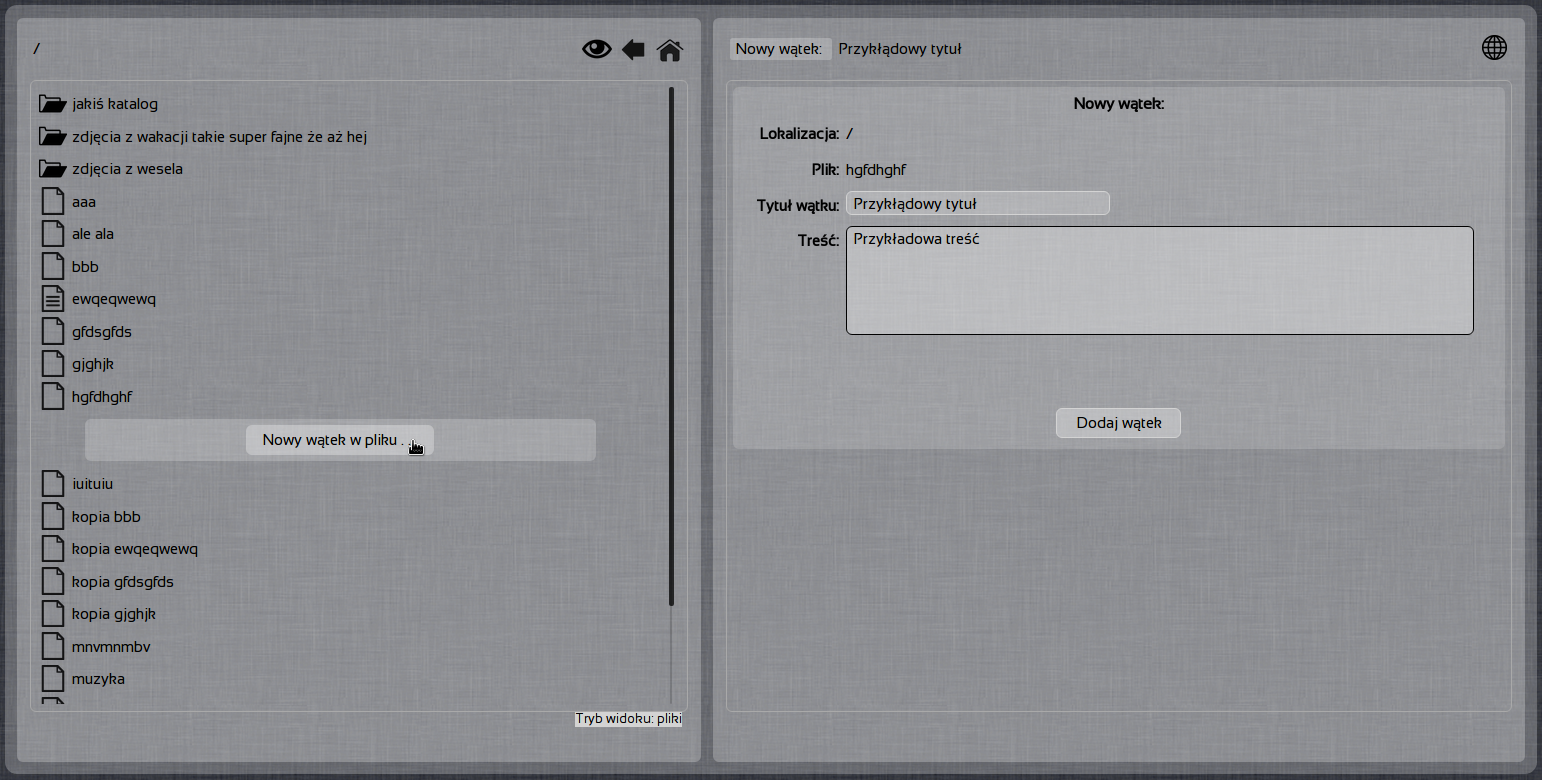
\includegraphics[width=400pt]{figures/screenshotnewthread1.png}
  \end{center}
  \caption{Zrzut ekranu z interfejsu graficznego podczas tworzenia nowego wątku.}
\end{figure}

Aby utworzyć nowy wątek w systemie, należy wykonać następujące kroki w sekcji plików:

\begin{enumerate}[noitemsep]
  \item Nawigując wewnątrz sekcji plików, znaleźć żądaną lokalizację wątku (lub żądany plik, któłrego ma dotyczyć dyskusja).
  
  \item Kliknąć kursorem myszy przycisk ,,\emph{Nowy wątek}'' (lub ,,\emph{Nowy wątek w pliku}'').
\end{enumerate}

Po wykonaniu powyższych czynności, następne kroki należy wykonać wewnątrz sekcji komentarzy, gdzie pojawią się puste pola tekstowe: ,,\emph{Tytuł wątku}'' oraz ,,\emph{Treść komentarza}'':

\begin{enumerate}[noitemsep]
  \item Uzupełnić wyżej wymienione pola tekstowe (w przypadku nie wypełnienia, zostanie wyświetlony odpowiedni komunikat).
  
  \item Zatwierdzić utworzenie nowego wątku przyciskiem ,,\emph{Dodaj wątek}''
\end{enumerate}

\subsection*{Wprowadzanie nowego komentarza}

\begin{figure}[h!]
  \vspace{5pt}
  \begin{center}
    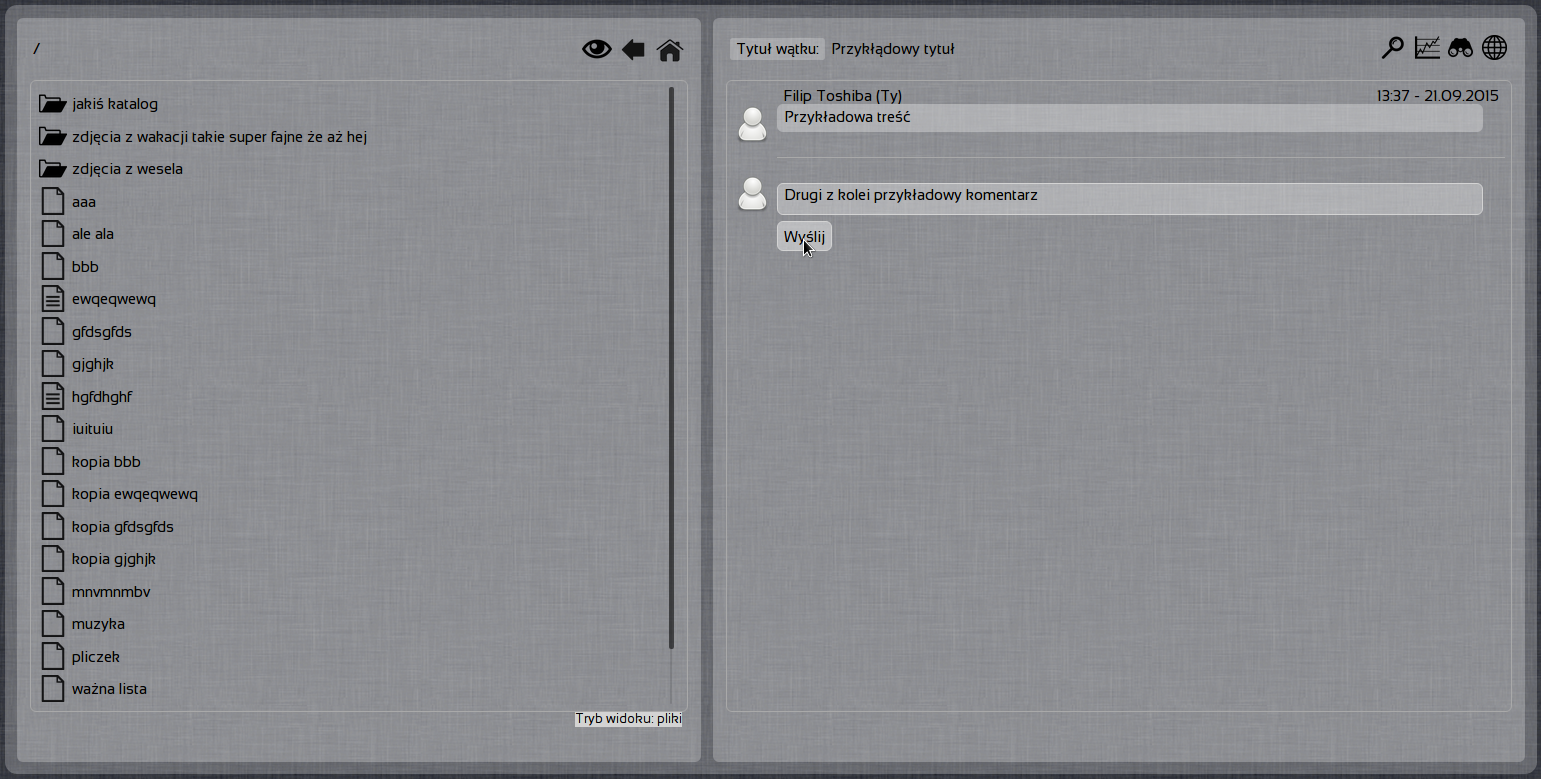
\includegraphics[width=400pt]{figures/screenshotnewcomment1.png}
  \end{center}
  \caption{Zrzut ekranu z interfejsu graficznego podczas dodawania nowego komentarza.}
\end{figure}

Podczas dodawania nowego komentarza użytkownik musi brać pod uwagę ograniczenie systemu polegające na tym, że aby umieścić nową wypowiedź, użytkownik powinien się znajdować w widoku aktualnego wątku (dokładny opis widoków znajduje się w sekcji \ref{views}). Jest to konieczne ze względu na fakt, iż nie będąc w widoku wątku, system nie będzie mógł umieścić komentarza w systemie plików, ponieważ nie będzie wiedział, w którym wątku stworzyć plik z nowym komentarzem.

Aby dodać nowy komentarz w dyskusji, użytkownik musi wykonać nastepujące kroki:

\begin{enumerate}[noitemsep]
  \item Po wyświetleniu komnetarzy z jednej dyskusji, użytkownik powinien przejść na sam dół sekcji komentarzy (tam, gdzie znajduje się najświeższa wypowiedź).
  
  \item Kliknięciem kursora myszy aktywować pole tekstowe i wpisać do niego treść wypowiedzi.
  
  \item Zatwierdzić komentarz przyciskiem ,,\emph{Dodaj}''.
\end{enumerate}

\subsection*{Modyfikacja komentarza}

\begin{figure}[h!]
  \vspace{5pt}
  \begin{center}
    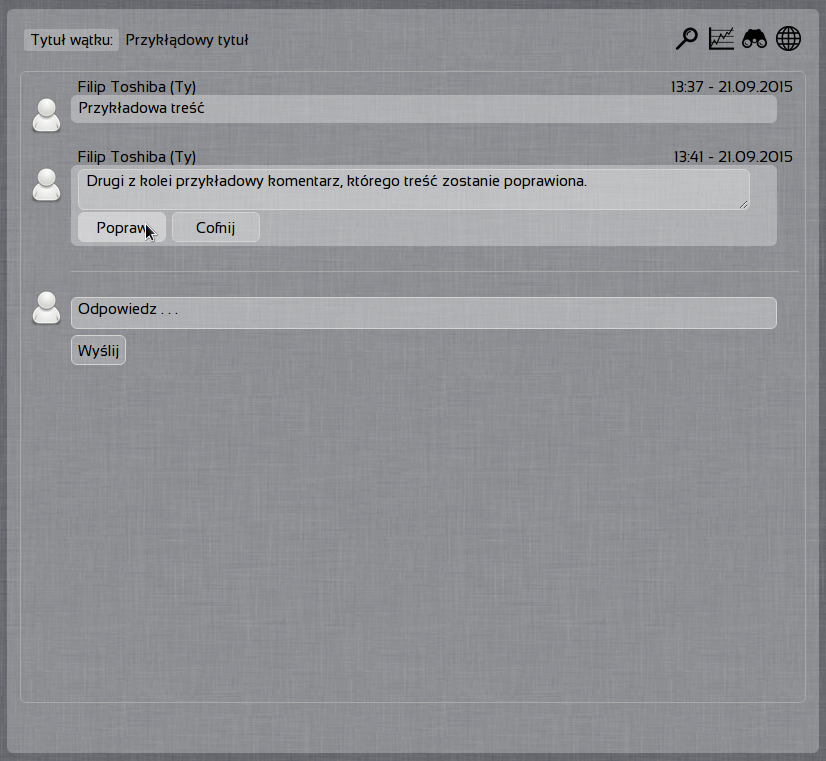
\includegraphics[width=240pt]{figures/screenshoteditcomment1.png}
  \end{center}
  \caption{Zrzut ekranu z interfejsu graficznego podczas edycji komentarza.}
\end{figure}

Jeśli użytkownik chce zmodyfikować treść komentarza, może tego dokonać, o ile jest jego autorem. Edycja treści odbywa się w sekcji komentarzy i przebiega w następujący sposób:

\begin{enumerate}[noitemsep]
  \item Po ustawieniu przez użytkownika kursora nad obszar komentarza wyświetlane są na nim przyciski inicjujące edycję oraz pokazujące historię zmian w jego treści (o ile zmiany kiedykolwiek nastąpiły).
  
  \item Po kliknięciu przycisku uruchamiającego edycję aktualny tekst komentarza umieszczany jest wewnątrz pola tekstowego, dodatkowo pojawia się przycisk akceptujący zmiany. Tekst jest edytowalny.
  
  \item Po wprowadzeniu zmian i zatwierdzeniu ich przyciskiem plik zk omentarzem jest modyfikowany.
\end{enumerate}

\newpage

\subsection*{Wyświetlanie historii zmian komentarza}

\begin{figure}[h!]
  \vspace{5pt}
  \begin{center}
    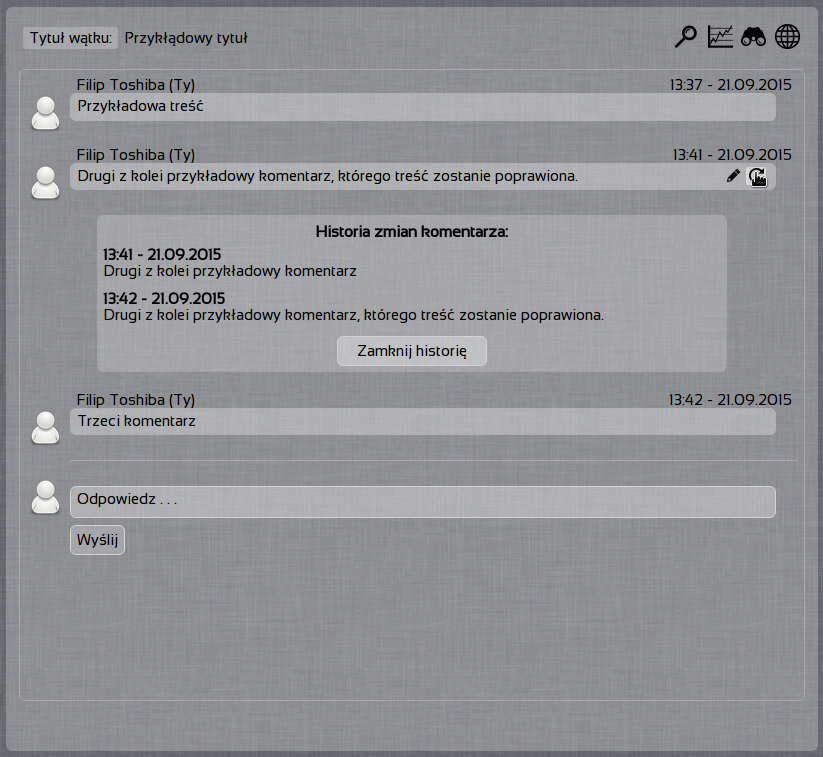
\includegraphics[width=240pt]{figures/screenshotcommenthistory1.png}
  \end{center}
  \caption{Zrzut ekranu z interfejsu graficznego podczas wyświetlania historii komentarza.}
\end{figure}

Przeglądanie historii zmian komentarzy jest możliwe tylko dla tych wypowiedzi, które zostały w przeszłości zmodyfikowane przez ich autorów. Historia może być wyświetlana przez każdego użytkownika w systemie. Przeglądanie modyfikacji odbywa się w sekcji komentarzy w następujący sposób:

\begin{enumerate}[noitemsep]
  \item Po ustawieniu przez użytkownika kursora nad obszar komentarza wyświetlane są na nim przyciski inicjujące edycję oraz pokazujące historię zmian w jego treści (o ile zmiany kiedykolwiek nastąpiły).
  
  \item Po uruchomieniu przycisku historii wyświetlona zostanie ramka pod komentarzem, zawierająca pełną treść komentarza po edycji, wraz z jej datą.
  
  \item Aby wyłączyć przeglądanie historii komentarza, należy kliknąć kursorem myszy na przycisk ,,\emph{Zamknij historię}'' wewnątrz ramki.
\end{enumerate}
% \input{chapters/0b-pisanie-w-latexu.tex}

% Bibliography (books, articles) starts here.
\bibliographystyle{plplain}{\raggedright\sloppy\small\bibliography{chapters/bibliography}}

% Colophon is a place where you should let others know about copyrights etc.
\ppcolophon

\end{document}
